\documentclass{article}

\usepackage{amsmath,geometry,graphicx,array,makecell,enumitem,bm,booktabs,multirow,pgfplots,bm,amssymb,mathtools,subcaption,cancel,adjustbox}
\usepackage[amsmath]{ntheorem}
\usepackage[hidelinks,naturalnames]{hyperref}
\usepackage[nameinlink,noabbrev]{cleveref}
\usepackage{fancyhdr}
\pagestyle{fancy}
\fancyhead[L]{\itshape\nouppercase{\leftmark}}
\fancyhead[R]{C6 Diffraction Methods in Chemistry}


\title{Diffraction Methods in Chemistry}
\author{Yue Wu}

\geometry{a4paper,hmargin=1.1in,vmargin=1.2in}

\setlength{\parskip}{1em}
\tolerance=1000
\emergencystretch=1em
\hyphenpenalty=1000
\exhyphenpenalty=100
\righthyphenmin=3

\theoremstyle{plain}\theoremheaderfont{\normalfont\itshape}\theorembodyfont{\rmfamily}\theoremseparator{.}\newtheorem*{rem}{Remark}\newtheorem*{ex}{Example}\newtheorem*{proof}{Proof}\newtheorem*{altp}{Alternative proof}

\theoremstyle{plain}\theoremheaderfont{\normalfont\bfseries}\theorembodyfont{\rmfamily}\theoremseparator{.}\newtheorem{thm}{Theorem}[section]\newtheorem{lem}[thm]{Lemma}\newtheorem{prop}[thm]{Proposition}\newtheorem*{cor}{Corollary}\newtheorem{defn}[thm]{Definition}\newtheorem{clm}[thm]{Claim}\newtheorem{clminproof}{Claim}\newtheorem*{law}{Law}\newtheorem{pos}[thm]{Postulate}

\theoremstyle{break}\theoremheaderfont{\normalfont\itshape}\theorembodyfont{\rmfamily}\theoremseparator{.\medskip}\newtheorem*{proofskip}{Proof}\newtheorem*{exs}{Examples}\newtheorem*{rems}{Remarks}

\theoremstyle{break}\theoremheaderfont{\normalfont\bfseries}\theorembodyfont{\rmfamily}\theoremseparator{.\medskip}\newtheorem{lemskip}[thm]{Lemma}\newtheorem{defnskip}[thm]{Definition}\newtheorem{propskip}[thm]{Proposition}\newtheorem{thmskip}[thm]{Theorem}

\crefname{thm}{Theorem}{Theorems}\crefname{defn}{Definition}{Definitions}\crefname{lem}{Lemma}{Lemmas}\crefname{lemskip}{Lemma}{Lemmas}\crefname{cor}{Corollary}{Corollaries} \crefname{prop}{Proposition}{Propositions}\crefname{clm}{Claim}{Claims}\crefname{pos}{Postulate}{Postulates}

\setcounter{tocdepth}{2}
\numberwithin{equation}{section}
\counterwithin{figure}{section}

\newcommand{\qed}{\hfill\ensuremath{\Box}}
\newcommand{\unit}[1]{\ \mathrm{#1}}
\newcommand{\ii}{\mathrm{i}}
\newcommand{\ee}{\mathrm{e}}
\newcommand{\tp}{^\mathrm{T}}
\newcommand{\dd}[2][]{\mathrm{d}^{#1} #2\,}
\renewcommand{\d}[2][]{\mathrm{d}^{#1} #2}
\newcommand{\dv}[3][]{\frac{\mathrm{d}^{#1} #2}{{\mathrm{d} #3}^{#1}}}
\newcommand{\pdv}[3][]{\frac{\partial^{#1} #2}{{\partial #3}^{#1}}}
\newcommand{\vb}[1]{\bm{\mathrm{#1}}}
\newcommand{\vu}[1]{\hat{\bm{\mathrm{#1}}}}
\newcommand{\vdot}{\,\bm{\mathrm{\cdot}}\,}
\newcommand{\cross}{\bm{\times}}
\newcommand{\abs}[1]{\left| #1 \right|}
\newcommand{\norm}[1]{\left\| #1 \right\|}
\newcommand{\grad}{\vb{\nabla}}
\renewcommand{\div}{\vb{\nabla}\cdot}
\newcommand{\curl}{\vb{\nabla}\times}
\newcommand{\laplacian}{\nabla^2}
\renewcommand{\Re}{\operatorname{Re}}
\renewcommand{\Im}{\operatorname{Im}}
\newcommand{\eval}[1]{\left\langle #1 \right\rangle}
\DeclareMathOperator{\Var}{Var}

\newcommand{\tikzAngleOfLine}{\tikz@AngleOfLine}
    \def\tikz@AngleOfLine(#1)(#2)#3{%
    \pgfmathanglebetweenpoints{%
        \pgfpointanchor{#1}{center}}{%
        \pgfpointanchor{#2}{center}}
    \pgfmathsetmacro{#3}{\pgfmathresult}%
}

\tikzset{
    screw/.pic={
        \draw[very thick] (0,-0.2) arc (-26.565:45:0.4472);
        \draw[very thick] (0,0.2) arc (153.435:225:0.4472);
        \fill[black] (0,-0.2) arc (-26.565:26.565:0.4472)--(0,0.2) arc (153.435:206.565:0.4472);
    },
}


\pgfplotsset{compat=1.18}
\usetikzlibrary{calc, math, arrows.meta}

\begin{document}
    \setlength{\parindent}{0pt}
	\Huge\textsf{\textbf{Diffraction Methods in Chemistry}}
		
	\Large\textsf{\textbf{University of Cambridge Part II Natural Sciences Tripos}}

	\noindent\makebox[\linewidth]{\rule{\textwidth}{2pt}}

	\large\textsf{\textbf{Yue Wu}}
	\begin{itemize}[topsep=0pt,leftmargin=15pt]
		\item[] \textit{Yusuf Hamied Department of Chemistry\\
		Lensfield Road,\\
		Cambridge, CB2 1EW}\\

		\textit{yw628@cam.ac.uk}
	\end{itemize}
    \thispagestyle{empty}
    \pagenumbering{roman}
    \setlength{\parindent}{15pt}

    \newpage
    \begin{center}
		\textbf{\Large{Acknowledgements}}
	\end{center}
	\large
	Nothing in these lecture notes is original. They are largely based on the notes by Dr. Andrew Bond, who lectured this course in 2025. They are nowhere near accurate representations of what was actually lectured, and in particular, all errors are almost surely mine.

    \normalsize
    \newpage
	\tableofcontents
	\newpage
    \pagenumbering{arabic}

    \section{Diffraction}
    It might be familiar from physics that if you shine a beam of light on a diffraction grating, then a diffraction pattern will emerge. If you put a lens after the diffracted beam, they may be brought to a focus, and a magnified image of the diffraction grating will be seen, as shown in the figure.

    \begin{figure}
        \centering
        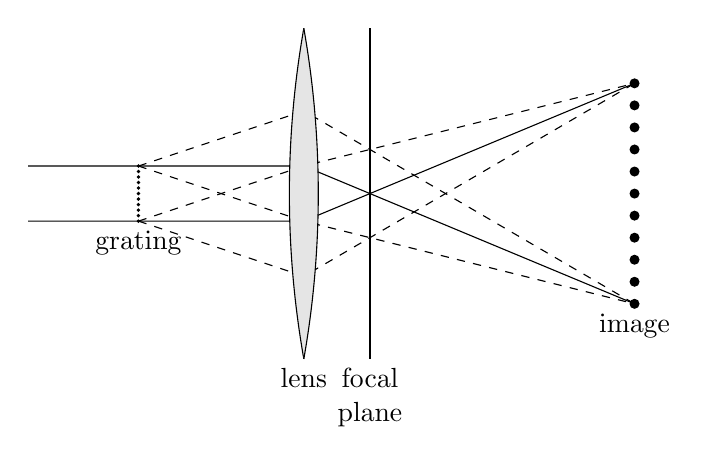
\begin{tikzpicture}[scale=0.7]
            \draw (0,0.5)--(5,0.5)--(11,-2);
            \draw (0,-0.5)--(5,-0.5)--(11,2);
            \draw[dashed] (2,0.5)--(5,1.5)--(11,-2);
            \draw[dashed] (2,-0.5)--(5,0.5)--(11,2);
            \draw[dashed] (2,-0.5)--(5,-1.5)--(11,2);
            \draw[dashed] (2,0.5)--(5,-0.5)--(11,-2);
            \draw[fill=gray!20] (5.0001,3) arc (170:190:17.276);
            \draw[fill=gray!20] (4.9999,-3) node[below]{lens} arc (-10:10:17.276);
            \foreach \i in {-5,...,5}{
                \draw[fill=black] (2,0.1*\i) circle (0.02);
                \draw[fill=black] (11,0.4*\i) circle (0.08);
            }
            \draw (6.2,-3)node[below,align=center]{focal \\ plane}--(6.2,3);
            \node at (2,-0.5)[below]{grating};
            \node at (11,-2)[below]{image};
        \end{tikzpicture}
        \caption{A magnified image of the diffraction grating is formed using a convex lens to focus the diffraction pattern.}
    \end{figure}

    Atoms in a crystal are, in some sense, very fine gratings. Can we use a similar method to image the atoms in a crystal directly? However, to form a diffraction pattern, we need the wavelength of the light to be in roughly the same length scale as the pattern we are trying to image. The atoms are on the order of Angstroms (\(10^{-10}\unit{m}\)), therefore, we need to use X-rays for diffraction at atomic length scales. However, there is no practical conventional lens for X-rays, because lenses are made of atoms too, so the imaging process does not work. What we have to do is to measure the intensity of the diffracted beams at different directions, and infer the atomic structure mathematically.

    This is, however, a hard thing to do. We will spend the vast majority of our lectures on how to translate the diffracted beam intensities into atomic structure.

    \subsection{Addition of Electromagnetic Waves}
    X-rays are electromagnetic waves, so they are described by Maxwell's equations, from which we can infer that the electromagnetic fields are essentially just oscillating electric and magnetic fields, travelling in some direction along the wavevector \(\vb{k}\) (the magnitude of \(\vb{k}\) also encodes the wavelength via \(\norm{\vb{k}}=2\pi/\lambda\)) with the speed of light \(c\).\footnote{In free space, \(\rho=0\) and \(\vb{J}=0\), so by Maxwell's equations
    \begin{equation}
        \curl(\curl\vb{E})=-\curl\pdv{\vb{B}}{t}=-\pdv{}{t}(\curl B)=-\pdv{}{t}\left(\mu_0\epsilon_0\pdv{\vb{E}}{t}\right)=-\mu_0\epsilon_0\pdv[2]{\vb{E}}{t}\,.
    \end{equation}
    By vector calculus identities, we also have
    \begin{equation}
        \curl(\curl\vb{E})=\grad(\div\vb{E})-\laplacian\vb{E}=-\laplacian\vb{E}\,,
    \end{equation}
    and hence
    \begin{equation}
        \laplacian\vb{E}=\mu_0\epsilon_0\pdv[2]{\vb{E}}{t}\,.
    \end{equation}
    This is the wave equation, with wave speed \(c=1/\sqrt{\mu_0\epsilon_0}\), with general complex solution
    \begin{equation}
        \vb{E}=\vb{E}_0\ee^{\ii(\vb{k}\cdot\vb{r}-\omega t)}
    \end{equation}
    for \(\vb{E}\in\mathbb{C}\) and \(\vb{k}^2 c^2=\omega^2\). By Maxwell's equations, we also have
    \begin{equation}
        \pdv{\vb{B}}{t}=-\curl\vb{E}=-\ii\vb{k}\times\vb{E}\,,
    \end{equation}
    and so
    \begin{equation}
        \vb{B}=\frac{\vb{k}}{\omega}\times\vb{E}\,.
    \end{equation}
    Therefore, \(\vb{E}\) and \(\vb{B}\) are both transverse waves that are in the same phase but perpendicular to each other.} We label the coordinate \(x\) along the propagation direction \(\vb{k}\), and consider the wave at some fixed time \(t\). Then the electric (or equivalently the magnetic) field strength is given by
    \begin{equation}
        \psi(x)=A\sin\left(\frac{2\pi x}{\lambda}+\phi\right)\,,
    \end{equation}
    where the real number \(A\) is the amplitude and \(\phi\) is the phase offset. However, it turns out that when considering oscillations, it is always easier to use complex numbers, so we will alternatively see the electric field as the real part of the complex wave
    \begin{equation}
        \psi(x)=A\exp\left(\frac{2\pi \ii x}{\lambda}\right)\,,
    \end{equation}
    where \(A=\abs{A}\ee^{\ii\phi}\) is now complex and includes both the amplitude \(\abs{A}\) and the initial phase offset \(\phi\).

    \begin{figure}
        \centering
        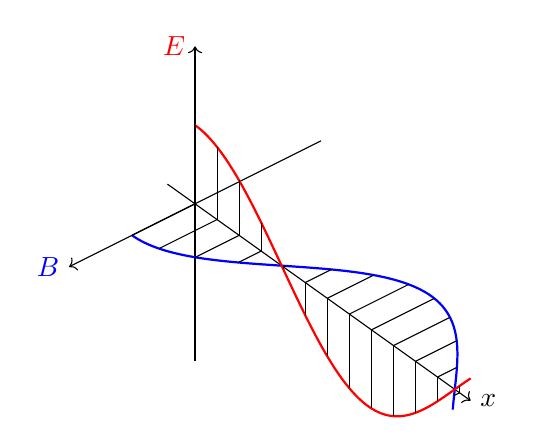
\begin{tikzpicture}[x={(-0.8cm,-0.4cm)},y={(0cm,1cm)},z={(0.7cm,-0.5cm)}]
            \draw[->] (-2,0)--(2,0)node[left,blue]{\(B\)};
            \draw[->] (0,-2)--(0,2)node[left,red]{\(E\)};
            \draw[->] (0,0,-0.5)--(0,0,5)node[right]{\(x\)};
            \draw[thick,domain=0:6.25, smooth, variable=\x,samples=50,blue] plot ({cos(0.8*\x r)}, {0}, {0.8*\x});
            \draw[thick,domain=0:6.25, smooth, variable=\x,samples=50,red] plot ({0}, {cos(0.8*\x r)}, {0.8*\x});
            \foreach \x in {0,...,12}{
                \draw (0,0,0.4*\x)--({cos(0.4*\x r)},0,0.4*\x);
                \draw (0,0,0.4*\x)--(0,{cos(0.4*\x r)},0.4*\x);
            }
        \end{tikzpicture}
        \caption{Electromagnetic wave propagating in space.}
    \end{figure}

    \begin{figure}[ht!]
        \centering
        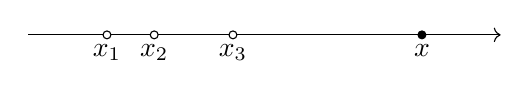
\begin{tikzpicture}
            \draw[->] (0,0)--(6,0);
            \draw[fill=white] (1,0)node[below]{\(x_1\)} circle (0.05);
            \draw[fill=white] (1.6,0)node[below]{\(x_2\)} circle (0.05);
            \draw[fill=white] (2.6,0)node[below]{\(x_3\)} circle (0.05);
            \draw[fill=black] (5,0)node[below]{\(x\)} circle (0.05);
        \end{tikzpicture}
    \end{figure}

    Now what happens if we have multiple sources, each sending off electromagnetic waves of the same frequencies but with different amplitudes and phases? Let's consider the simple 1D case, where \(n\) sources are located at \(x_j\). We will let all \(n\) sources have a zero initial phase\footnote{It is a trivial generalisation for the sources to have different non-zero initial phases. We make such assumption because this is the only situation we will need for later discussion, and it makes my diagram cleaner. It is actually also trivial to generalise it to 3D by replacing \(x-x_j\) with \(\norm{\vb{x}-\vb{x}_j}\) in all the expressions below.}, so that the resulting wave at point \(x\) due to source \(j\) is given by
    \begin{equation}
        \psi_j(x)=A_j\exp\left(\frac{2\pi \ii(x-x_j)}{\lambda}\right)\,,
    \end{equation}
    where \(A_j\) is real because we have a zero initial phase. We will denote the phase of the wave due to source \(j\) at \(x\) as
    \begin{equation}
        \phi_j=\frac{2\pi(x-x_j)}{\lambda}\,.
    \end{equation}
    Then to work out the total wave, we only need to sum up the contributions from each source to get
    \begin{equation}
        \Psi_{\text{res}}(x)=\sum_jA_j\exp\left(\ii\phi_j\right)\,.
    \end{equation}
    It is easy to see that the phase angle of the resultant amplitude is
    \begin{equation}
        \Phi_{\text{res}}=\tan^{-1}\left[\frac{\sum_j A_j\sin \phi_j}{\sum_j A_j \cos\phi_j}\right]\,.
    \end{equation}

    \begin{figure}[ht!]
        \centering
        \begin{tikzpicture}
            \draw[->] (-0.5,0)--(4,0)node[right]{\(\Re\Psi\)};
            \draw[->] (0,-0.5)--(0,4)node[left]{\(\Im\Psi\)};
            \coordinate (A) at (0,0);
            \coordinate (B) at ($(A)+(35:1.5)$);
            \coordinate (C) at ($(B)+(55:1.7)$);
            \coordinate (D) at ($(C)+(92:1.9)$);
            \draw[->,thick] (A)--node[above]{\small\(A_1\)}(B);
            \draw[->,thick] (B)--node[left]{\small\(A_2\)}(C);
            \draw[->,thick] (C)--node[left]{\small\(A_3\)}(D);
            \draw[->,thick] (A)--node[left]{\(\abs{\Psi_{\text{res}}}\)}(D);
            \draw[dashed] (B)-- +(1,0);
            \draw[dashed] (C)-- +(1,0);

            \tikzAngleOfLine(A)(B){\AngleB}
            \draw (A)+(0.5,0) arc (0:\AngleB:0.5 cm) node[midway,right] {\(\phi_1\)};
            \tikzAngleOfLine(B)(C){\AngleC}
            \draw (B)+(0.5,0) arc (0:\AngleC:0.5 cm) node[midway,right] {\(\phi_2\)};
            \tikzAngleOfLine(C)(D){\AngleD}
            \draw (C)+(0.5,0) arc (0:\AngleD:0.5 cm) node[midway,right] {\(\phi_3\)};
        \end{tikzpicture}
    \end{figure}

    Now what if we move the measuring point \(x\) by an amount of \(\delta x\)? This will increase the phases of the wave from all the sources by
    \begin{equation}
        \delta\phi=\frac{2\pi\delta x}{\lambda}\,.
    \end{equation}
    The net result is that the resultant magnitude of the combined wave does not change, but the phase changes by \(\delta\phi\), as
    \begin{equation}
        \Psi'_{\text{res}}(x)=\sum_jA_j\exp(\ii(\phi_j+\delta\phi))=\ee^{\ii\delta\phi}\sum_jA_j\exp(\ii\phi_j)\,.
    \end{equation}
    
    \begin{figure}[ht!]
        \centering
        \begin{tikzpicture}
            \draw[->] (-0.5,0)--(4,0)node[right]{\(\Re\Psi\)};
            \draw[->] (0,-0.5)--(0,4)node[right]{\(\Im\Psi\)};
            \coordinate (A) at (0,0);
            \coordinate (B) at ($(A)+(95:1.5)$);
            \coordinate (C) at ($(B)+(115:1.7)$);
            \coordinate (D) at ($(C)+(152:1.9)$);
            \coordinate (P) at ($(A)+(60:1)$);
            \coordinate (Q) at ($(B)+(60:1)$);
            \coordinate (R) at ($(C)+(60:1)$);
            \draw[->,thick] (A)--node[left]{\small\(A_1\)}(B);
            \draw[->,thick] (B)--node[left]{\small\(A_2\)}(C);
            \draw[->,thick] (C)--node[below]{\small\(A_3\)}(D);
            \draw[->,thick] (A)--node[left]{\(\abs{\Psi_{\text{res}}}\)}(D);
            \draw[dashed] (A)--(P);
            \draw[dashed] (Q)--(B)-- +(1,0);
            \draw[dashed] (R)--(C)-- +(1,0);
            \tikzAngleOfLine(A)(P){\AngleDelta}
            \tikzAngleOfLine(A)(B){\AngleB}
            \draw (A)+(60:0.5) arc (\AngleDelta:\AngleB:0.5 cm) node[midway,above] {\(\phi_1\)};
            \tikzAngleOfLine(B)(C){\AngleC}
            \draw (B)+(60:0.5) arc (\AngleDelta:\AngleC:0.5 cm) node[midway,above] {\(\phi_2\)};
            \tikzAngleOfLine(C)(D){\AngleD}
            \draw (C)+(60:0.5) arc (\AngleDelta:\AngleD:0.5 cm) node[midway,above] {\(\phi_3\)};
            \draw (A)+(0:0.5) arc (0:\AngleDelta:0.5 cm) node[midway,right] {\(\delta\phi\)};
            \draw (B)+(0:0.5) arc (0:\AngleDelta:0.5 cm) node[midway,right] {\(\delta\phi\)};
            \draw (C)+(0:0.5) arc (0:\AngleDelta:0.5 cm) node[midway,right] {\(\delta\phi\)};
        \end{tikzpicture}
        \caption{Movement of the measuring point results in a change of measured phase only.}
    \end{figure}

    What if we change the position of one of the sources \(x_k\)? This will in general lead to a change in the phase \(\phi_k\). Now both the phase and the amplitude of the resulting wave is different.

    \begin{figure}[ht!]
        \centering
        \begin{tikzpicture}
            \draw[->] (-0.5,0)--(4,0)node[right]{\(\Re\Psi\)};
            \draw[->] (0,-0.5)--(0,4)node[left]{\(\Im\Psi\)};
            \coordinate (A) at (0,0);
            \coordinate (B) at ($(A)+(35:1.5)$);
            \coordinate (C) at ($(B)+(55:1.7)$);
            \coordinate (D) at ($(C)+(150:1.9)$);
            \draw[->,thick] (A)--node[above]{\small\(A_1\)}(B);
            \draw[->,thick] (B)--node[left]{\small\(A_2\)}(C);
            \draw[->,thick] (C)--node[left]{\small\(A_3\)}(D);
            \draw[->,thick] (A)--node[left]{\(\abs{\Psi_{\text{res}}}\)}(D);
            \draw[dashed] (B)-- +(1,0);
            \draw[dashed] (C)-- +(1,0);

            \tikzAngleOfLine(A)(B){\AngleB}
            \draw (A)+(0.5,0) arc (0:\AngleB:0.5 cm) node[midway,right] {\(\phi_1\)};
            \tikzAngleOfLine(B)(C){\AngleC}
            \draw (B)+(0.5,0) arc (0:\AngleC:0.5 cm) node[midway,right] {\(\phi_2\)};
            \tikzAngleOfLine(C)(D){\AngleD}
            \draw (C)+(0.5,0) arc (0:\AngleD:0.5 cm) node[midway,above] {\(\phi_3\)};
        \end{tikzpicture}
        \caption{A change in the position of one of the sources leads to a change in both the magnitude and the phase measured.}
    \end{figure}

    \subsection{Diffraction of an Object}
    We would now like to consider the diffraction of an extended object. Suppose we have parallel incident beams from the direction \(\vu{s}_0\) illuminating the whole object, and we are measuring the diffracted beam at some distant point \(Q\). The dimension of this object is small compared to its distance to the measuring point \(Q\) so we can sensibly say that \(Q\) is at direction \(\vu{s}\) for all points in the object.\footnote{This type of diffraction is known as \textit{Fraunhofer diffraction}. If you are observing near the diffracting object, then the diffraction is \textit{Fresnel diffraction}.} Moreover, we assume that the effect of diffraction is weak, so the diffraction only happens once --- an already diffracted beam cannot be diffracted again. This is known as the \textit{kinematic approximation}.\footnote{If this assumption is false (as it will be for electron diffractions), we need to consider a more complicated \textit{dynamic scattering}.}
    
    To produce the diffraction pattern, we need to sum up the radiation scattered from all the points in the object. To do this, we first pick an arbitrary origin \(O\) in the object, and we need to figure out the intensity and phase difference between the beams diffracted in direction \(\vu{s}\) from \(O\) and from any other point \(P\) with position vector \(\vb{r}\).

    \begin{figure}
        \centering
        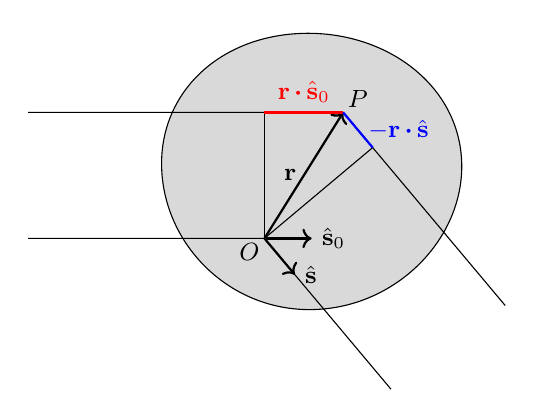
\begin{tikzpicture}
            \draw[fill=gray!30] plot[smooth cycle, tension=1] coordinates{(-1.3,0) (0.4,1.8) (2.5,0.25) (0.7,-1.7)};
            \draw (-3,-0.8)--(0,-0.8)--+(-50:2.5);
            \draw (-3,0.8)--(1,0.8)--+(-50:3.2);
            \draw[->,thick] (0,-0.8)node[below left=-2pt]{\small\(O\)}--node[left=-1pt]{\small\(\vb{r}\)}(1,0.8)node[above right=-2pt]{\small\(P\)};
            \draw (0,-0.8)--(0,0.8);
            \draw (0,-0.8)--+(40:1.795);
            \draw[->,thick] (0,-0.8)--(0.6,-0.8)node[right]{\small\(\vu{s}_0\)};
            \draw[->,thick] (0,-0.8)--+(-50:0.6)node[right]{\small\(\vu{s}\)};
            \draw[thick,red] (0,0.8)--node[above,red]{\small\(\vb{r}\vdot\vu{s}_0\)}(1,0.8);
            \draw[thick,blue] (1,0.8)--node[right,blue]{\small\(-\vb{r}\vdot\vu{s}\)}+(-50:0.583);
        \end{tikzpicture}
        \caption{Path difference for diffractions in a general object.}
        \label{object_diffraction}
    \end{figure}

    From \cref{object_diffraction}, it is easy to see that the beam diffracted from \(P\) and \(O\) has a path difference
    \begin{equation}
        \Delta x=\vb{r}\vdot\vu{s}_0-\vb{r}\vdot\vu{s}\,.
    \end{equation}
    In particular, a positive path difference means that the beam from \(P\) falls behind the beam from \(O\), leading to a negative phase difference, so
    \begin{equation}
        \Delta\phi=-\frac{2\pi\Delta x}{\lambda}=\frac{2\pi\vb{r}\vdot(\vu{s}-\vu{s}_0)}{\lambda}\,.
    \end{equation}
    The amplitude of the beam diffracted from \(O\) and \(P\) may also be different, since the object may be inhomogeneous. Let \(A(\vb{r})\) be a real function representing the diffraction amplitude, then by integrating over all points, the wave measured at point \(Q\) is
    \begin{equation}
        \Psi(\vu{s})=\int\dd[3]{\vb{r}}A(\vb{r})\exp\left(\frac{2\pi \ii\vb{r}\vdot(\vu{s}-\vu{s}_0)}{\lambda}\right)\,.
    \end{equation}
    The integral is over the object volume.

    We can define the \textit{scattering vector} \(\vb{S}\) by
    \begin{equation}
        \vb{S}\coloneqq\frac{\vu{s}-\vu{s}_0}{\lambda}\,.
    \end{equation}
    It is a vector bisecting the external angle between the incident and diffracted beam, as shown in the figure below. If we define the angle of deflection to be \(2\theta\), then the length of the scattering vector is
    \begin{equation}
        \norm{\vb{S}}=\frac{2\sin\theta}{\lambda}\,.
    \end{equation}
    The scattering vector has dimension \([\mathrm{L}]^{-1}\), so it exists in the reciprocal space, which might be familiar from Part IB Chemistry A.\footnote{In some derivation, one uses \textit{momentum transfer vector} \(\vb{Q}\) defined by
    \begin{equation}
        \vb{Q}=\frac{2\pi(\vu{s}-\vu{s}_0)}{\lambda}\,.
    \end{equation}
    instead of \(\vb{S}\).}
    \begin{figure}[ht!]
        \centering
        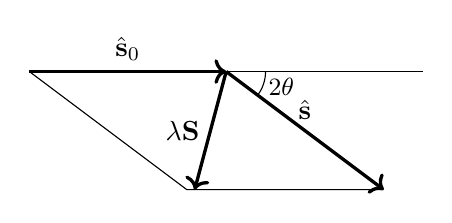
\begin{tikzpicture}
            \draw (-2.5,0)--(2.5,0);
            \draw[very thick,->] (-2.5,0)--node[above]{\(\vu{s}_0\)}(0,0);
            \draw[very thick,->] (0,0)--node[above]{\(\vu{s}\)}(2,-1.5);
            \draw (-2.5,0)--(-0.5,-1.5)--(2,-1.5);
            \draw[very thick,->] (0,0)--node[left]{\(\lambda\vb{S}\)}(-0.4,-1.5);
            \draw (0.5,0) arc (0:-36.87:0.5);
            \node at (0.7,-0.2){\small \(2\theta\)};
        \end{tikzpicture}
        \caption{Construction of the scattering vector.}
    \end{figure}
    
    This allows us to simplify our expression of the measured wave as
    \begin{equation}
        \Psi(\vb{S})=\int\dd[3]{\vb{r}}A(\vb{r})\exp\left(2\pi \ii\vb{r}\vdot\vb{S}\right)\,.
    \end{equation}

    \subsection{Diffraction of X-rays from Electrons}
    We will now consider how X-rays interacts with matter. The interaction generally fall into two categories.
    \begin{itemize}[topsep=0pt]
        \item \textit{Elastic scattering.} This is our main focus. In an \textit{elastic scattering}, or \textit{Thomson scattering}, there is no net transfer of energy from the photon to the material. It can be thought of as some kind of resonance of the atomic electrons. When X-rays pass through the material, the oscillating electric field causes the atomic electrons to oscillate, which in turn emit X-rays in all directions. The incoming and outgoing rays retain a non-random phase relationship and are said to be \textit{coherent}.
        \item \textit{Inelastic processes.} \textit{Inelastic processes} involve energy transfer from the incoming X-rays to electrons in atoms. The simplest example is photoelectron emission, where an X-ray photon providing energy for an atom to eject a core-shell electron. The photons are then re-emitted with lower energy in an incoherent fashion. This incoherence means that they cannot interfere with each other to produce diffraction patterns. Other processes of this type may result from interaction with valence shell electrons or vibrations, all being incoherent. We are therefore not interested in inelastic processes at this stage --- we will return to this later.
    \end{itemize}

    The quantitative description of Thomson scattering strictly only applies to free electrons, but the results are found to be generally applicable to crystals under normal scattering conditions. Crucially, the amplitude of X-rays diffracted from some point is proportional to the local electron density \(\rho(\vb{r})\). Therefore,
    \begin{equation}
        \Psi(\vb{S})=\int\dd[3]{\vb{r}}\sigma\rho(\vb{r})\exp(2\pi \ii\vb{r}\vdot\vb{S})\,,
    \end{equation}
    where \(\sigma\) is the scattering power of a single electron. We can divide through this constant of proportionality to obtain the \textit{structure factor} \(F(\vb{S})\) given by
    \begin{equation}
        F(\vb{S})=\int\dd[3]{\vb{r}}\rho(\vb{r})\exp\left(2\pi \ii\vb{r}\vdot\vb{S}\right)\,.
    \end{equation}
    The limits of the two integrals above are both throughout the whole 3D space. Mathematically, \(F(\vb{S})\) is the \textit{Fourier transform} of the electron density \(\rho(\vb{r})\).
    \begin{defn}
        Let \(f:\mathbb{R}^n\to\mathbb{C}\) be a function. The \textit{Fourier transform} of \(f\) is \(\mathcal{F}[f]\equiv\tilde{f}:\mathbb{R}^n\to\mathbb{C}\) given by\footnote{You might be more familiar with the Fourier transform defined as
        \begin{equation}
            \tilde{f}=\frac{1}{\sqrt{2\pi}}\int\dd{x}f(x)\ee^{-ikx}\,,
        \end{equation}
        where the normalisation factor of \(1/\sqrt{2\pi}\) may or may not be there. It is just a matter of convention. However, this difference in convention is annoying since it results in slight tweaks in a lot of formulae.}
        \begin{equation}
            \tilde{f}(\vb{k})\coloneqq\int\dd[n]{\vb{x}}f(\vb{x})\ee^{2\pi \ii\vb{k}\vdot\vb{x}}\,.
        \end{equation}
    \end{defn}
    \begin{thm}
        Let \(\tilde{f}(\vb{k})\) be the Fourier transform of \(f(\vb{x})\). The \textit{inverse Fourier transform} that converts \(\tilde{f}\) back to \(f\) is given by
        \begin{equation}
            f(\vb{x})=\mathcal{F}^{-1}[\tilde{f}(\vb{k})]\coloneqq\int\dd[3]{\vb{k}}\tilde{f}(\vb{k})\ee^{-2\pi \ii\vb{k}\vdot\vb{x}}\,.
        \end{equation}
    \end{thm}
    \begin{proof}
        \begin{align}
            \mathcal{F}^{-1}[\tilde{f}](\vb{x})&=\int\dd[n]{\vb{k}}\ee^{-2\pi \ii\vb{k}\vdot\vb{x}}\int\dd[3]{\vb{s}}\ee^{2\pi \ii\vb{k}\vdot\vb{s}}f(\vb{s})\notag \\
            &=\int\dd[n]{\vb{s}}f(\vb{s})\int\dd[n]{\vb{k}}\ee^{2\pi \ii k\vdot(\vb{s}-\vb{x})}\notag\\
            &=\int\dd[n]{\vb{s}}f(\vb{s})\delta(\vb{s}-\vb{x})\notag\\
            &=f(\vb{x})\,.
        \end{align}\qed
    \end{proof}
    Hence to convert the \(F(\vb{S})\) back to \(\rho(\vb{r})\), one simply needs to perform the inverse Fourier transform
    \begin{equation}
        \rho(\vb{r})=\int\dd[3]{\vb{S}}F(\vb{S})\exp(-2\pi \ii\vb{r}\vdot\vb{S})\,.
    \end{equation}
    Again, the integral is throughout the whole 3D space, and it is omitted.

    This means that if we can determine the \(F(\vb{S})\), then we can easily reconstruct the electron density in a material, no matter how complex the structure is. (1) Measure the phases and the amplitudes of the diffracted beams. (2) Divide by single-electron scattering power \(\sigma\) to get \(F(\vb{S})\). (3) Do the inverse Fourier transform to obtain \(\rho(\vb{r})\). Simple as that! Three steps to solve any chemical structure in the world!

    This should be the happy ending of our story on X-ray diffraction.

    \newpage
    \section{The Phase Problem and the Patterson Function}
    \subsection{The Phase Problem}
    If the problem is really that simple, then this would be a one-lecture course instead of a 12-lecture one. There is a huge issue. We cannot measure the phase of an X-ray.

    To measure the magnitude and the phase of an electromagnetic wave, we would use an antenna. However, this requires the antenna to have its dimensions comparable to the radiation wavelength. The X-rays we used for diffraction are at atomic length scale --- that's why we can see the diffraction, but it is impossible to make an antenna at atomic length scale since antennas should be made from atoms! All we can measure in a diffraction experiment is the number of X-ray photons encountered in a given time, which is the diffracted \textit{intensity}. This is proportional to \(I=\abs{F(\vb{S})}^2\). The phase information is completely lost. This is referred to as the \textit{phase problem} in diffraction.

    Now the question is: is getting the correct phase important? If using a wrong phase of the diffracted beam has little impact on the electron density calculated, then this would not be a huge problem. We can calculate the modulus of \(F(\vb{S})\) by taking the square root of the intensity, and just plug in some random phases to calculate \(\rho(\vb{r})\). However, it turns out that getting the correct phase is extremely important --- it even plays a more important role than the magnitude to some extent. This can be illustrated by the following little experiment.

    Instead of doing Fourier transform of a electron density function, we do a Fourier transform on a picture. A black and white picture is also a function of the pixels, where the values of the function is the gray scale. We can transform it into the frequency domain, and then transform it back, and we get the original image. However, if we use some randomly generated phase values to replace the correct phase values in the Fourier transform of the image, and we transform it back, we see a complete mess. This is what will happen if we use random phase values for the structure factor --- we will get no valuable information. In fact, if we use some random value for the magnitudes of the Fourier transform, with the correct phase values, we can still vaguely see the shape of a cat.
    \begin{figure}[ht!]
        \begin{subfigure}[h]{0.3\linewidth}
            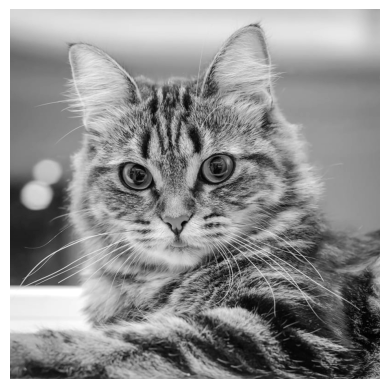
\includegraphics[width=\linewidth]{cat_norm.png}
            \caption{Correct magnitudes + correct phases}
        \end{subfigure}
        \hfill
        \begin{subfigure}[h]{0.3\linewidth}
            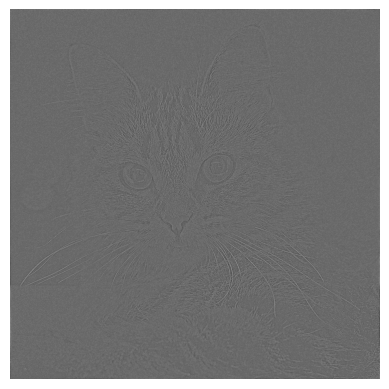
\includegraphics[width=\linewidth]{cat_rand_mod.png}
            \caption{Random magnitudes + correct phases}
        \end{subfigure}
        \hfill
        \begin{subfigure}[h]{0.3\linewidth}
            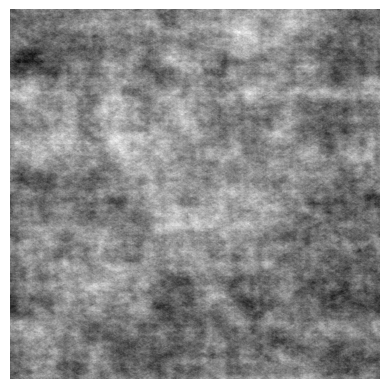
\includegraphics[width=\linewidth]{cat_rand_ph.png}
            \caption{Correct magnitudes + random phases}
        \end{subfigure}%
        \caption{The effect of using the wrong phases and magnitudes in an inverse Fourier transform.}
    \end{figure}

    Just for fun, we can extend this experiment further. We have two images: one is a benzene molecule and the other is a cat. What will happen if we use the magnitude value of one figure with the phase value of the other? The result is shown in (\ref{Fig:cat_and_benzene}), and you can see it is the phase that determines what we will see. In general, we don't want to see a cat if we are investigating the structure of benzene using diffraction, so it's not a good idea just to use a random set of phases when doing inverse Fourier transform.
    \begin{figure}[ht!]
        \begin{subfigure}[h]{0.45\linewidth}
            \centering
            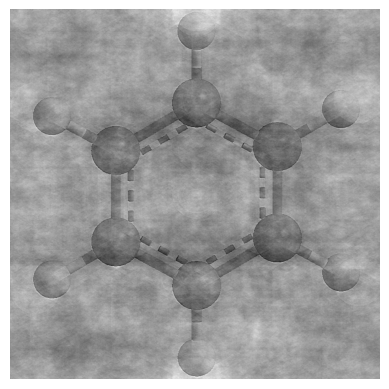
\includegraphics[width=0.8\linewidth]{cat_with_ben.png}
            \caption{Magnitudes of cat + phases of benzene}
        \end{subfigure}
        \hfill
        \begin{subfigure}[h]{0.45\linewidth}
            \centering
            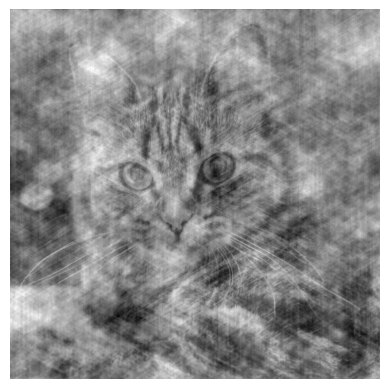
\includegraphics[width=0.8\linewidth]{ben_with_cat.png}
            \caption{Magnitudes of benzene + phases of cat}
        \end{subfigure}
        \caption{Phases govern what we see in an inverse Fourier transform. If you use the phases of a benzene, you see a benzene. If you use the phases of a cat, you see a cat.}
        \label{Fig:cat_and_benzene}
    \end{figure}

    Moral: phases are important, but we can't measure them. The main task of structure determination using X-ray diffraction is to deduce the phases of the structure factor. This is what we will spend the remaining 11 lectures on.

    \subsection{Patterson Function}
    Since all what we can get from measuring a diffraction pattern is the intensity \(I(\vb{S})=\abs{F(\vb{S})}^2\), let's see what its inverse Fourier transform gives us anyway.

    Before doing that, let's first introduce convolution and correlation.

    \begin{defn}
        For two functions \(f,g:\mathbb{R}^n\to\mathbb{C}\), their \textit{convolution} is
        \begin{equation}
            (f*g)(\vb{x})\coloneqq\int\dd[n]{\vb{s}}f(\vb{s})g(\vb{x}-\vb{s})\,,
        \end{equation}
        and their \textit{correlation} is
        \begin{equation}
            (f\otimes g)(\vb{x})\coloneqq\int\dd[n]{\vb{s}}f(\vb{s})^*g(\vb{x}+\vb{s})\,.
        \end{equation}
    \end{defn}
    \begin{figure}[ht!]
        \centering
        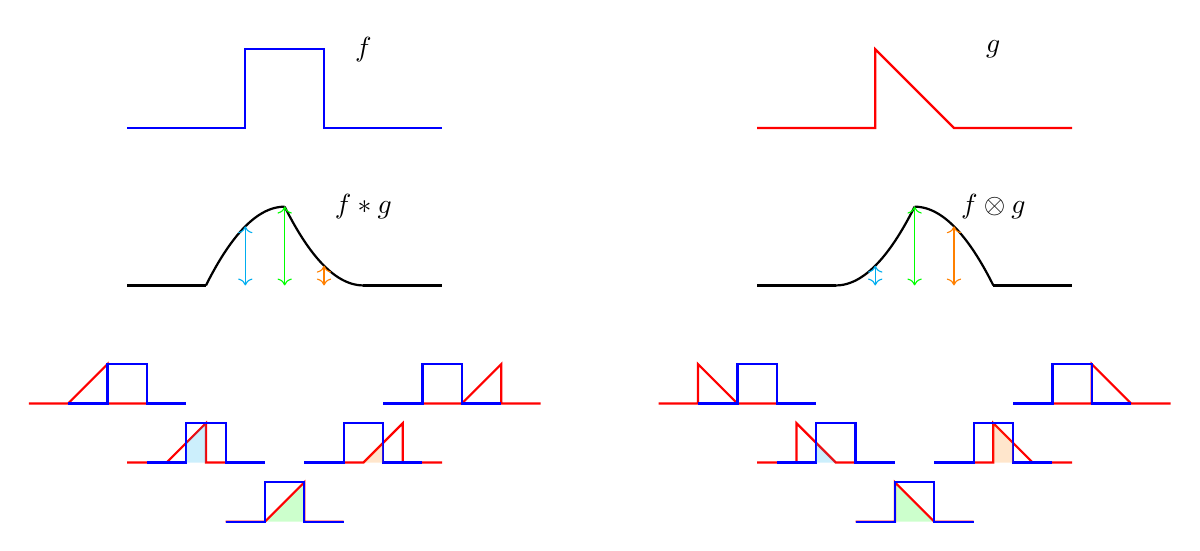
\begin{tikzpicture}
            \begin{scope}[shift={(-4,2)}]
                \draw[blue,thick] (-2,0)--(-0.5,0)--(-0.5,1)--(0.5,1)--(0.5,0)--(2,0);
                \node at (1,1){\(f\)};
            \end{scope}
            \begin{scope}[shift={(4,2)}]
                \draw[red,thick] (-2,0)--(-0.5,0)--(-0.5,1)--(0.5,0)--(2,0);
                \node at (1,1){\(g\)};
            \end{scope}
            \begin{scope}[shift={(-4,0)}]
                \draw[thick] (-2,0)--(-1,0);
                \draw[thick] (1,0)--(2,0);
                \draw[thick,domain=-1:0, smooth, variable=\x,samples=50] plot ({\x}, {1-\x*\x});
                \draw[thick,domain=0:1, smooth, variable=\x,samples=50] plot ({\x}, {(1-\x)*(1-\x)});
                \node at (1,1){\(f*g\)};
                \draw[<->,cyan] (-0.5,0)--(-0.5,0.75);
                \draw[<->,green] (0,0)--(0,1);
                \draw[<->,orange] (0.5,0)--(0.5,0.25);
            \end{scope}
            \begin{scope}[shift={(-6,-1.5)},scale=0.5]
                \draw[red,thick,xshift=-1cm] (-1.5,0)--(-0.5,0)--(0.5,1)--(0.5,0)--(1.5,0);
                \draw[blue,thick] (-1.5,0)--(-0.5,0)--(-0.5,1)--(0.5,1)--(0.5,0)--(1.5,0);
            \end{scope}
            \begin{scope}[shift={(-5,-2.25)},scale=0.5]
                \draw[red,thick,xshift=-0.5cm] (-1.5,0)--(-0.5,0)--(0.5,1)--(0.5,0)--(1.5,0);
                \draw[blue,thick] (-1.5,0)--(-0.5,0)--(-0.5,1)--(0.5,1)--(0.5,0)--(1.5,0);
                \fill[cyan,fill opacity=0.2] (-0.5,0.5)--(0,1)--(0,0)--(-0.5,0);
            \end{scope}
            \begin{scope}[shift={(-4,-3)},scale=0.5]
                \draw[red,thick,fill=green, fill opacity=0.2] (-1.5,0)--(-0.5,0)--(0.5,1)--(0.5,0)--(1.5,0);
                \draw[blue,thick] (-1.5,0)--(-0.5,0)--(-0.5,1)--(0.5,1)--(0.5,0)--(1.5,0);
            \end{scope}
            \begin{scope}[shift={(-3,-2.25)},scale=0.5]
                \draw[red,thick,xshift=0.5cm] (-1.5,0)--(-0.5,0)--(0.5,1)--(0.5,0)--(1.5,0);
                \draw[blue,thick] (-1.5,0)--(-0.5,0)--(-0.5,1)--(0.5,1)--(0.5,0)--(1.5,0);
                \fill[orange, fill opacity=0.2] (0.5,0.5)--(0.5,0)--(0,0);
            \end{scope}
            \begin{scope}[shift={(-2,-1.5)},scale=0.5]
                \draw[red,thick,xshift=1cm] (-1.5,0)--(-0.5,0)--(0.5,1)--(0.5,0)--(1.5,0);
                \draw[blue,thick] (-1.5,0)--(-0.5,0)--(-0.5,1)--(0.5,1)--(0.5,0)--(1.5,0);
            \end{scope}

            \begin{scope}[shift={(4,0)}]
                \draw[thick] (-2,0)--(-1,0);
                \draw[thick] (1,0)--(2,0);
                \draw[thick,domain=0:1, smooth, variable=\x,samples=50] plot ({\x}, {1-\x*\x});
                \draw[thick,domain=-1:0, smooth, variable=\x,samples=50] plot ({\x}, {(1+\x)*(1+\x)});
                \node at (1,1){\(f\otimes g\)};
                \draw[<->,cyan] (-0.5,0)--(-0.5,0.25);
                \draw[<->,green] (0,0)--(0,1);
                \draw[<->,orange] (0.5,0)--(0.5,0.75);
            \end{scope}
            \begin{scope}[shift={(2,-1.5)},scale=0.5]
                \draw[red,thick,xshift=-1cm] (-1.5,0)--(-0.5,0)--(-0.5,1)--(0.5,0)--(1.5,0);
                \draw[blue,thick] (-1.5,0)--(-0.5,0)--(-0.5,1)--(0.5,1)--(0.5,0)--(1.5,0);
            \end{scope}
            \begin{scope}[shift={(3,-2.25)},scale=0.5]
                \draw[red,thick,xshift=-0.5cm] (-1.5,0)--(-0.5,0)--(-0.5,1)--(0.5,0)--(1.5,0);
                \draw[blue,thick] (-1.5,0)--(-0.5,0)--(-0.5,1)--(0.5,1)--(0.5,0)--(1.5,0);
                \fill[cyan,fill opacity=0.2] (-0.5,0.5)--(0,0)--(-0.5,0);
            \end{scope}
            \begin{scope}[shift={(4,-3)},scale=0.5]
                \draw[red,thick,fill=green, fill opacity=0.2] (-1.5,0)--(-0.5,0)--(-0.5,1)--(0.5,0)--(1.5,0);
                \draw[blue,thick] (-1.5,0)--(-0.5,0)--(-0.5,1)--(0.5,1)--(0.5,0)--(1.5,0);
            \end{scope}
            \begin{scope}[shift={(5,-2.25)},scale=0.5]
                \draw[red,thick,xshift=0.5cm] (-1.5,0)--(-0.5,0)--(-0.5,1)--(0.5,0)--(1.5,0);
                \draw[blue,thick] (-1.5,0)--(-0.5,0)--(-0.5,1)--(0.5,1)--(0.5,0)--(1.5,0);
                \fill[orange, fill opacity=0.2] (0,1)--(0.5,0.5)--(0.5,0)--(0,0);
            \end{scope}
            \begin{scope}[shift={(6,-1.5)},scale=0.5]
                \draw[red,thick,xshift=1cm] (-1.5,0)--(-0.5,0)--(-0.5,1)--(0.5,0)--(1.5,0);
                \draw[blue,thick] (-1.5,0)--(-0.5,0)--(-0.5,1)--(0.5,1)--(0.5,0)--(1.5,0);
            \end{scope}
        \end{tikzpicture}
        \caption{Graphic explanation of convolution and correlation.}
    \end{figure}

    \begin{thm}[Convolution theorem]
        The Fourier transform of a convolution is the product of Fourier transforms.
        \begin{equation}
            \mathcal{F}[f*g]=\mathcal{F}[f]\mathcal{F}[g]\,.
        \end{equation}
    \end{thm}
    \begin{proof}
        \begin{align}
            \mathcal{F}[f*g](\vb{k})&=\int\dd[n]{\vb{x}}\ee^{2\pi \ii\vb{k}\vdot\vb{x}}\int\dd[n]{\vb{s}}f(\vb{s})g(\vb{x}-\vb{s})\notag\\
            &=\int\dd[n]{\vb{s}}f(\vb{s})\int\dd[n]{\vb{x}}\ee^{2\pi \ii\vb{k}\vdot\vb{x}}g(\vb{x}-\vb{s})\notag\\
            &=\int\dd[n]{\vb{s}}f(\vb{s})\int\dd[n]{\vb{u}}\ee^{2\pi \ii\vb{k}\vdot(\vb{u}+\vb{s})}g(\vb{u}) \qquad\text{define }\vb{u}=\vb{x}-\vb{s}\notag \\
            &=\int\dd[n]{\vb{s}}\ee^{2\pi \ii\vb{k}\vdot\vb{s}}f(\vb{s})\int\dd[n]{\vb{u}}\ee^{2\pi \ii\vb{k}\vdot\vb{u}}g(\vb{u})\notag \\
            &=\tilde{f}(\vb{k})\tilde{g}(\vb{k})\,.
        \end{align}\qed
    \end{proof}
    \begin{thm}
        Conversely, the Fourier transform of a product \(fg\) is the convolution of their Fourier transforms
        \begin{equation}
            \mathcal{F}[fg]=\mathcal{F}[f]*\mathcal{F}[g]\,.
        \end{equation}
    \end{thm}
    \begin{proof}
        \begin{align}
            \mathcal{F}[fg](\vb{k})&=\int\dd[n]{\vb{x}}\ee^{2\pi \ii\vb{k}\vdot\vb{x}}f(\vb{x})g(\vb{x})\notag \\
            &=\int\dd[n]{\vb{x}}\ee^{2\pi \ii\vb{k}\vdot\vb{x}}f(\vb{x})\int\dd[n]{\vb{\ell}}\ee^{-2\pi \ii\vb{\ell}\vdot\vb{x}}\tilde{g}(\vb{\ell})\notag \\
            &=\int\dd[n]{\vb{\ell}}\tilde{g}(\vb{\ell})\int\dd[n]{\vb{x}}\ee^{2\pi \ii\vb{x}\vdot(\vb{k}-\vb{\ell})}f(\vb{x})\notag \\
            &=\int\dd[n]{\vb{\ell}}\tilde{g}(\vb{\ell})\tilde{f}(\vb{k}-\vb{\ell})\notag \\
            &=\tilde{f}*\tilde{g}(\vb{k})\,.
        \end{align}\qed
    \end{proof}
    We see a beautiful duality here. Product in the real domain is the convolution in the Fourier domain, and \textit{vice versa}.
    \begin{thm}[Wiener--Khinchin theorem]
        The Fourier transform of the autocorrelation of a function is its \textit{power spectral intensity}.
        \begin{equation}
            \mathcal{F}[f\otimes f]=\abs{\tilde{f}}^2\,.
        \end{equation}
    \end{thm}
    \begin{proof}
        \begin{align}
            \mathcal{F}[f\otimes f](\vb{k})&=\int\dd[n]{\vb{x}}\ee^{2\pi \ii\vb{k}\vdot\vb{x}}\int\dd[n]{\vb{s}}f^*(\vb{s})f(\vb{x}+\vb{s})\notag\\
            &=\int\dd[n]{\vb{s}}f^*(\vb{s})\int\dd[n]{\vb{x}}\ee^{2\pi \ii\vb{k}\vdot\vb{x}}f(\vb{x}+\vb{s})\notag\\
            &=\int\dd[n]{\vb{s}}f^*(\vb{s})\int\dd[n]{\vb{u}}\ee^{2\pi \ii\vb{k}\vdot(\vb{u}-\vb{s})}f(\vb{u}) \qquad\text{define }\vb{u}=\vb{x}+\vb{s}\notag \\
            &=\int\dd[n]{\vb{s}}\ee^{-2\pi \ii\vb{k}\vdot\vb{s}}f^*(\vb{s})\int\dd[n]{\vb{u}}\ee^{2\pi \ii\vb{k}\vdot\vb{u}}f(\vb{u})\notag \\
            &=\tilde{f}^*(\vb{k})\tilde{f}(\vb{k})=\abs{\tilde{f}(\vb{k})}^2\,.
        \end{align}\qed
    \end{proof}
    Finally, if we apply both sides on the Wiener--Khinchin theorem, we get
    \begin{equation}
        \mathcal{F}^{-1}\left[|\tilde{f}|^2\right]=f\otimes f\,.
    \end{equation}
    We can apply this to our diffraction intensity! We previously identified the structure factor to be the Fourier transform of the electron density, \(F(\vb{S})=\mathcal{F}[\rho(\vb{x})]\), and the diffraction intensity is exactly \(I(\vb{S})=\abs{F(\vb{S})}^2\). Therefore, the inverse Fourier transform of the diffraction intensity is exactly the autocorrelation of the electron density!
    \begin{equation}
        \mathcal{F}^{-1}[I(\vb{S})]=\rho\otimes\rho(\vb{r})\,.
    \end{equation}
    We often call this the \textit{Patterson function}, denoted \(P(\vb{r})\).

    \subsection{Illustrating the Patterson Function}
    The above derivation is a bit abstract. Let's do a simple 1D example of an electron density function with three peaks, modelling three atoms in a line, and see how its Patterson function look like.

    \begin{figure}[ht!]
        \centering
        \begin{tikzpicture}
            \draw[->] (-4,0)--(4,0)node[above]{\(x\)};
            \draw[thick,domain=-1:0.6, smooth, variable=\x,samples=50] plot ({\x-1}, {2*2.72^(-50*\x*\x)});
            \draw[thick,domain=-0.6:1, smooth, variable=\x,samples=50] plot ({\x}, {3*2.72^(-50*\x*\x)});
            \draw[thick,domain=-1:1, smooth, variable=\x,samples=50] plot ({\x+1.5}, {2.72^(-50*\x*\x)});
            \node at (-1,2)[above]{\(1\)};
            \node at (0,3)[above]{\(2\)};
            \node at (1.5,1)[above]{\(3\)};
            \draw (-1,0.05)--(-1,0)node[below]{\small\(-1\)};
            \draw (0,0.05)--(0,0)node[below]{\small\(0\)};
            \draw (1.5,0.05)--(1.5,0)node[below]{\small\(1.5\)};
        \end{tikzpicture}
    \end{figure}

    We put the three peaks at positions \(x=-1\), \(x=0\) and \(x=1.5\) with weights \(2\), \(3\) and \(1\) respectively. From the definition of the Patterson function, which is the correlation of the electron density with itself
    \begin{equation}
        P(u)=\int\dd{x}\rho(x)\rho(x+u)\,,
    \end{equation}
    we need to take another copy of electron density function, shift it by some distance \(u\), and evaluate the integral of their product, which is roughly governed by how well do the peaks of the two functions overlap. Let's set \(u\) to a range of different values and see what happens.
    \begin{itemize}
        \item \(u=-3\): First, when \(u\) is very negative, the two function has almost no overlap, so at this value of \(u\), \(P(u)\approx 0\).
        \begin{figure}[ht!]
            \centering
            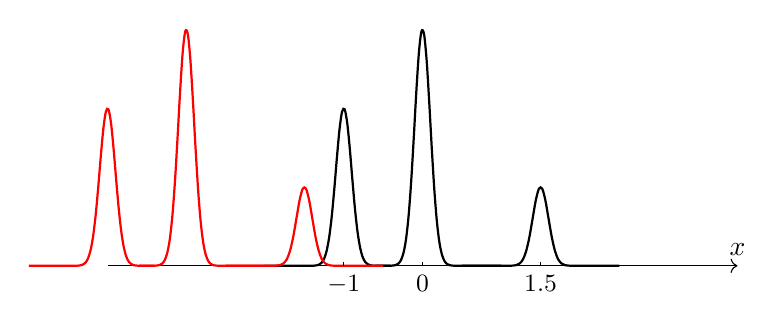
\begin{tikzpicture}
                \draw[->] (-4,0)--(4,0)node[above]{\(x\)};
                \draw[thick,domain=-1:0.6, smooth, variable=\x,samples=50] plot ({\x-1}, {2*2.72^(-50*\x*\x)});
                \draw[thick,domain=-0.6:1, smooth, variable=\x,samples=50] plot ({\x}, {3*2.72^(-50*\x*\x)});
                \draw[thick,domain=-1:1, smooth, variable=\x,samples=50] plot ({\x+1.5}, {2.72^(-50*\x*\x)});
                \begin{scope}[shift={(-3,0)}]
                    \draw[red,thick,domain=-1:0.6, smooth, variable=\x,samples=50] plot ({\x-1}, {2*2.72^(-50*\x*\x)});
                    \draw[red,thick,domain=-0.6:1, smooth, variable=\x,samples=50] plot ({\x}, {3*2.72^(-50*\x*\x)});
                    \draw[red,thick,domain=-1:1, smooth, variable=\x,samples=50] plot ({\x+1.5}, {2.72^(-50*\x*\x)});
                \end{scope}
                \draw (-1,0.05)--(-1,0)node[below]{\small\(-1\)};
                \draw (0,0.05)--(0,0)node[below]{\small\(0\)};
                \draw (1.5,0.05)--(1.5,0)node[below]{\small\(1.5\)};
            \end{tikzpicture}
        \end{figure}
        \item \(u=-2.5\): At this value of \(u\), peak 1 and peak 3 just overlaps. Without the actual functional form of the peak, we can't evaluate this integral of their product, but since peak \(1\) has weight \(2\) and peak \(3\) has weight \(1\), we can roughly assign a relative weight of \(2\times 1=2\) to the Patterson function here.
        \begin{figure}[ht!]
            \centering
            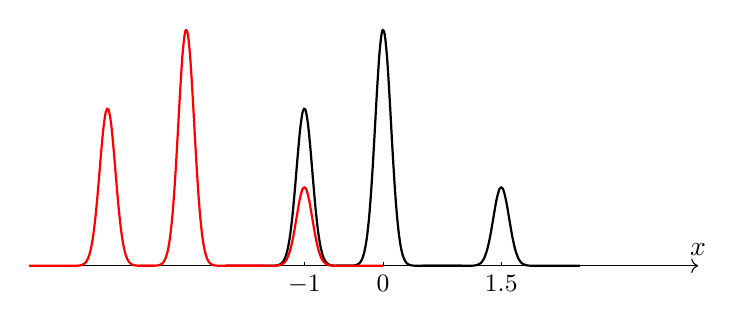
\begin{tikzpicture}
                \draw[->] (-4,0)--(4,0)node[above]{\(x\)};
                \draw[thick,domain=-1:0.6, smooth, variable=\x,samples=50] plot ({\x-1}, {2*2.72^(-50*\x*\x)});
                \draw[thick,domain=-0.6:1, smooth, variable=\x,samples=50] plot ({\x}, {3*2.72^(-50*\x*\x)});
                \draw[thick,domain=-1:1, smooth, variable=\x,samples=50] plot ({\x+1.5}, {2.72^(-50*\x*\x)});
                \begin{scope}[shift={(-2.5,0)}]
                    \draw[red,thick,domain=-1:0.6, smooth, variable=\x,samples=50] plot ({\x-1}, {2*2.72^(-50*\x*\x)});
                    \draw[red,thick,domain=-0.6:1, smooth, variable=\x,samples=50] plot ({\x}, {3*2.72^(-50*\x*\x)});
                    \draw[red,thick,domain=-1:1, smooth, variable=\x,samples=50] plot ({\x+1.5}, {2.72^(-50*\x*\x)});
                \end{scope}
                \draw (-1,0.05)--(-1,0)node[below]{\small\(-1\)};
                \draw (0,0.05)--(0,0)node[below]{\small\(0\)};
                \draw (1.5,0.05)--(1.5,0)node[below]{\small\(1.5\)};
            \end{tikzpicture}
        \end{figure}
        \item \(u=-1.5\): Now at this value of \(u\), peak 3 and peak 2 overlaps, giving a peak in the Patterson function with relative weight \(3\times 1=3\).\\
        \begin{figure}[ht!]
            \centering
            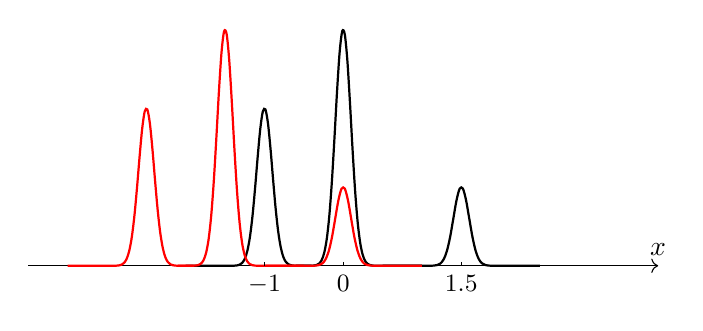
\begin{tikzpicture}
                \draw[->] (-4,0)--(4,0)node[above]{\(x\)};
                \draw[thick,domain=-1:0.6, smooth, variable=\x,samples=50] plot ({\x-1}, {2*2.72^(-50*\x*\x)});
                \draw[thick,domain=-0.6:1, smooth, variable=\x,samples=50] plot ({\x}, {3*2.72^(-50*\x*\x)});
                \draw[thick,domain=-1:1, smooth, variable=\x,samples=50] plot ({\x+1.5}, {2.72^(-50*\x*\x)});
                \begin{scope}[shift={(-1.5,0)}]
                    \draw[red,thick,domain=-1:0.6, smooth, variable=\x,samples=50] plot ({\x-1}, {2*2.72^(-50*\x*\x)});
                    \draw[red,thick,domain=-0.6:1, smooth, variable=\x,samples=50] plot ({\x}, {3*2.72^(-50*\x*\x)});
                    \draw[red,thick,domain=-1:1, smooth, variable=\x,samples=50] plot ({\x+1.5}, {2.72^(-50*\x*\x)});
                \end{scope}
                \draw (-1,0.05)--(-1,0)node[below]{\small\(-1\)};
                \draw (0,0.05)--(0,0)node[below]{\small\(0\)};
                \draw (1.5,0.05)--(1.5,0)node[below]{\small\(1.5\)};
            \end{tikzpicture}
        \end{figure}
        \item \(u=-1\): Peak 1 and peak 2 overlap, giving a peak in the Patterson function with relative weight \(2\times 3=6\).
        \begin{figure}[ht!]
            \centering
            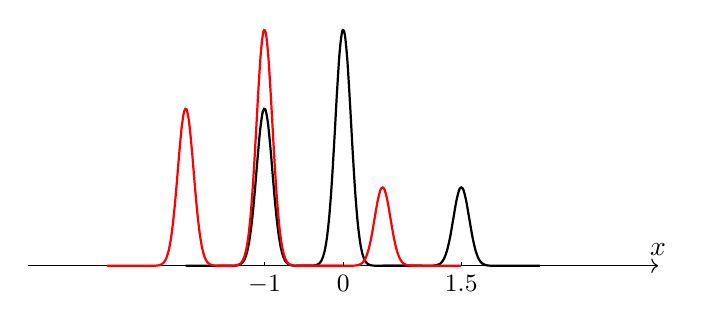
\begin{tikzpicture}
                \draw[->] (-4,0)--(4,0)node[above]{\(x\)};
                \draw[thick,domain=-1:0.6, smooth, variable=\x,samples=50] plot ({\x-1}, {2*2.72^(-50*\x*\x)});
                \draw[thick,domain=-0.6:1, smooth, variable=\x,samples=50] plot ({\x}, {3*2.72^(-50*\x*\x)});
                \draw[thick,domain=-1:1, smooth, variable=\x,samples=50] plot ({\x+1.5}, {2.72^(-50*\x*\x)});
                \begin{scope}[shift={(-1,0)}]
                    \draw[red,thick,domain=-1:0.6, smooth, variable=\x,samples=50] plot ({\x-1}, {2*2.72^(-50*\x*\x)});
                    \draw[red,thick,domain=-0.6:1, smooth, variable=\x,samples=50] plot ({\x}, {3*2.72^(-50*\x*\x)});
                    \draw[red,thick,domain=-1:1, smooth, variable=\x,samples=50] plot ({\x+1.5}, {2.72^(-50*\x*\x)});
                \end{scope}
                \draw (-1,0.05)--(-1,0)node[below]{\small\(-1\)};
                \draw (0,0.05)--(0,0)node[below]{\small\(0\)};
                \draw (1.5,0.05)--(1.5,0)node[below]{\small\(1.5\)};
            \end{tikzpicture}
        \end{figure}
        \item \(u=0\): At this special value of \(u\), the second function is not moved at all, so all the three peaks are perfectly aligned. This leads to a very large peak in the Patterson function with weight \(2^2+3^2+1^2=14\).
        \begin{figure}[ht!]
            \centering
            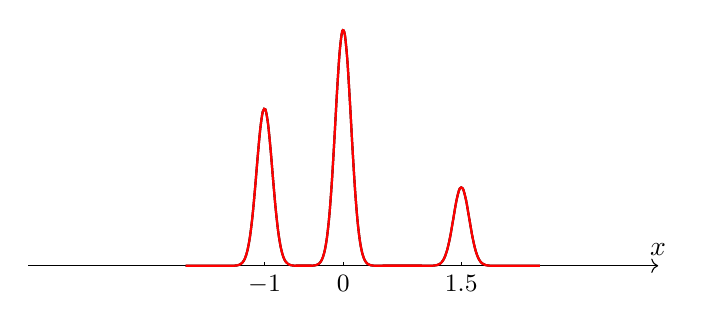
\begin{tikzpicture}
                \draw[->] (-4,0)--(4,0)node[above]{\(x\)};
                \draw[thick,domain=-1:0.6, smooth, variable=\x,samples=50] plot ({\x-1}, {2*2.72^(-50*\x*\x)});
                \draw[thick,domain=-0.6:1, smooth, variable=\x,samples=50] plot ({\x}, {3*2.72^(-50*\x*\x)});
                \draw[thick,domain=-1:1, smooth, variable=\x,samples=50] plot ({\x+1.5}, {2.72^(-50*\x*\x)});
                \begin{scope}
                    \draw[red,thick,domain=-1:0.6, smooth, variable=\x,samples=50] plot ({\x-1}, {2*2.72^(-50*\x*\x)});
                    \draw[red,thick,domain=-0.6:1, smooth, variable=\x,samples=50] plot ({\x}, {3*2.72^(-50*\x*\x)});
                    \draw[red,thick,domain=-1:1, smooth, variable=\x,samples=50] plot ({\x+1.5}, {2.72^(-50*\x*\x)});
                \end{scope}
                \draw (-1,0.05)--(-1,0)node[below]{\small\(-1\)};
                \draw (0,0.05)--(0,0)node[below]{\small\(0\)};
                \draw (1.5,0.05)--(1.5,0)node[below]{\small\(1.5\)};
            \end{tikzpicture}
        \end{figure}
    \end{itemize}
    You can go further to check other values of \(u\), but we should have done enough to discover a pattern. The Patterson function will have peaks at the values when there are two peaks in the electron density function align, which are exactly the ``inter-peak'' distances in the electron density. The relative weight of the peak in the Patterson function is the product of the weight of the peaks in the electron density.

    \begin{figure}[ht!]
        \centering
        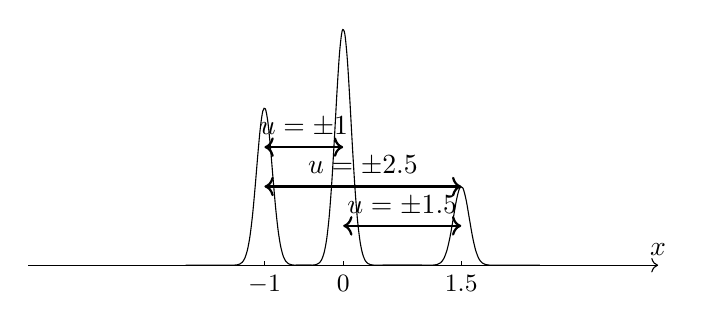
\begin{tikzpicture}
            \draw[->] (-4,0)--(4,0)node[above]{\(x\)};
            \draw[domain=-1:0.6, smooth, variable=\x,samples=50] plot ({\x-1}, {2*2.72^(-50*\x*\x)});
            \draw[domain=-0.6:1, smooth, variable=\x,samples=50] plot ({\x}, {3*2.72^(-50*\x*\x)});
            \draw[domain=-1:1, smooth, variable=\x,samples=50] plot ({\x+1.5}, {2.72^(-50*\x*\x)});
            \draw[<->,thick] (-1,1.5)--node[above]{\(u=\pm 1\)}(0,1.5);
            \draw[<->,thick] (-1,1)--node[above]{\(u=\pm 2.5\)}(1.5,1);
            \draw[<->,thick] (0,0.5)--node[above]{\(u=\pm 1.5\)}(1.5,0.5);
            \draw (-1,0.05)--(-1,0)node[below]{\small\(-1\)};
            \draw (0,0.05)--(0,0)node[below]{\small\(0\)};
            \draw (1.5,0.05)--(1.5,0)node[below]{\small\(1.5\)};
        \end{tikzpicture}
        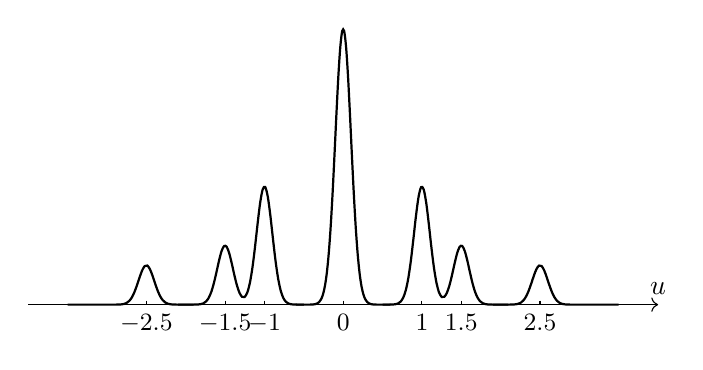
\begin{tikzpicture}
            \draw[->] (-4,0)--(4,0)node[above]{\(u\)};
            \draw[thick,domain=-1:0.6, smooth, variable=\x,samples=50] plot ({\x-2.5}, {0.5*2.72^(-50*\x*\x)});
            \draw[thick,domain=-0.6:1, smooth, variable=\x,samples=50] plot ({\x-1.5}, {0.75*2.72^(-50*\x*\x)+1.5*2.72^(-50*(\x-0.5)*(\x-0.5))});
            \draw[thick,domain=-0.6:0.6, smooth, variable=\x,samples=50] plot ({\x}, {3.5*2.72^(-50*\x*\x)});
            \draw[thick,domain=-1:0.6, smooth, variable=\x,samples=50] plot ({\x+1.5}, {0.75*2.72^(-50*\x*\x)+1.5*2.72^(-50*(\x+0.5)*(\x+0.5))});
            \draw[thick,domain=-0.6:1, smooth, variable=\x,samples=50] plot ({\x+2.5}, {0.5*2.72^(-50*\x*\x)});
            \draw (-2.5,0.05)--(-2.5,0)node[below]{\small\(-2.5\)};
            \draw (-1.5,0.05)--(-1.5,0)node[below]{\small\(-1.5\)};
            \draw (-1,0.05)--(-1,0)node[below]{\small\(-1\)};
            \draw (0,0.05)--(0,0)node[below]{\small\(0\)};
            \draw (1,0.05)--(1,0)node[below]{\small\(1\)};
            \draw (1.5,0.05)--(1.5,0)node[below]{\small\(1.5\)};
            \draw (2.5,0.05)--(2.5,0)node[below]{\small\(2.5\)};
        \end{tikzpicture}
        \caption{Peaks in the Patterson function correspond to the inter-peak vectors in the electron density function.}
    \end{figure}

    To conclude, let's summarise some features of the Patterson function:
    \begin{enumerate}[topsep=0pt]
        \item The Patterson function is defined in the same space as \(\rho(\vb{r})\) (as opposed to the structure factor defined in the reciprocal space), and it spans a range twice that spanned by \(\rho(\vb{r})\).
        \item The Patterson function is always centrosymmetric, even if \(\rho(\vb{r})\) is not.
        \item The maximum of the Patterson function occurs at \(\vb{u}=\vb{0}\), and its value is
        \begin{equation}
            P(\vb{0})=\int\dd[3]{\vb{r}}\rho^2(\vb{r})\,.
        \end{equation}
        \item Local maxima in \(P(\vb{u})\) occur when peaks in \(\rho(\vb{r})\) overlaps with those in \(\rho(\vb{u}+\vb{r})\). This happens if the offset vector \(\vb{u}\) is some peak\(\leftrightarrow\)peak vector in \(\rho(\vb{r})\). If we take an atomic picture of the electron density, in which electron densities are concentrated on the atomic sites (we will formalise this latter), then peaks in \(P(\vb{u})\) occur when \(\vb{u}\) is an \textit{interatomic vector}.
        \item If there are \(N\) peaks in \(\rho(\vb{r})\), there are \(N^2\) interatomic vectors. Of these, \(N\) will occur at \(\vb{u}=\vb{0}\), corresponding to vectors of an atom pointing itself. Consequently, there will in general be \(N^2-N\) non-origin peaks in \(P(\vb{u})\) (some of them may overlap as well).
        \item For a function \(\rho(\vb{r})\) consists of resolved peaks, the total weight (area) of the peak produced in \(P(\vb{u})\) is proportional to the product of the weights of the peaks in \(\rho(\vb{r})\) and \(\rho(\vb{r}+\vb{u})\) producing it. If atoms in \(\rho(\vb{r})\) and \(\rho(\vb{r}+\vb{u})\) have atomic numbers \(Z_1\) and \(Z_2\), then the weight of the peaks in \(P(\vb{u})\) will be proportional to \(Z_1 Z_2\). Consequently, Patterson peaks involving heavy atoms (where \(Z_1\) and/or \(Z_2\) is large) will show up most clearly.
        \item Peaks in \(P(\vb{u})\) will be broader than in \(\rho(\vb{r})\), and peaks corresponding to vectors from light atoms may merge into a poorly-defined background.
    \end{enumerate}

    Hence, as we will see later, the Patterson function will be helpful in locating heavy atoms in a structure.

    \subsection{Patterson Function of a Molecule}
    Now consider a \(\mathrm{SO_3}\) molecule. For simplicity, we will make this problem 2 dimensional. The atomic number of \(\mathrm{S}\) and \(\mathrm{O}\) are 16 and 8 respectively, so the electron density function has one peak of weight 16, which we set at the origin, and three peaks of weight 8 at the same distance from the origin, separated by \(120^\circ\).

    \begin{figure}[ht!]
        \centering
        \begin{tikzpicture}
            \draw[->] (-2.5,0)--(2.5,0);
            \draw[->] (0,-2.5)--(0,2.5);
            \draw (0,0)--+(30:1.5)node[above=0.4cm]{\(\mathrm{O1}\)};
            \draw (0,0)--+(150:1.5)node[above=0.4cm]{\(\mathrm{O2}\)};
            \draw (0,0)--+(270:1.5)node[right=0.4cm]{\(\mathrm{O3}\)};
            \draw[fill=white] (0,0) node{\small\(16\)} circle (0.42);
            \draw[fill=white] (30:1.5) node{\small\(8\)} circle (0.3);
            \draw[fill=white] (150:1.5) node{\small\(8\)} circle (0.3);
            \draw[fill=white] (270:1.5) node{\small\(8\)} circle (0.3);
        \end{tikzpicture}
        \caption{The electron density of a \(\mathrm{SO_3}\) molecule.}
    \end{figure}
    \begin{figure}[ht!]
        \centering
        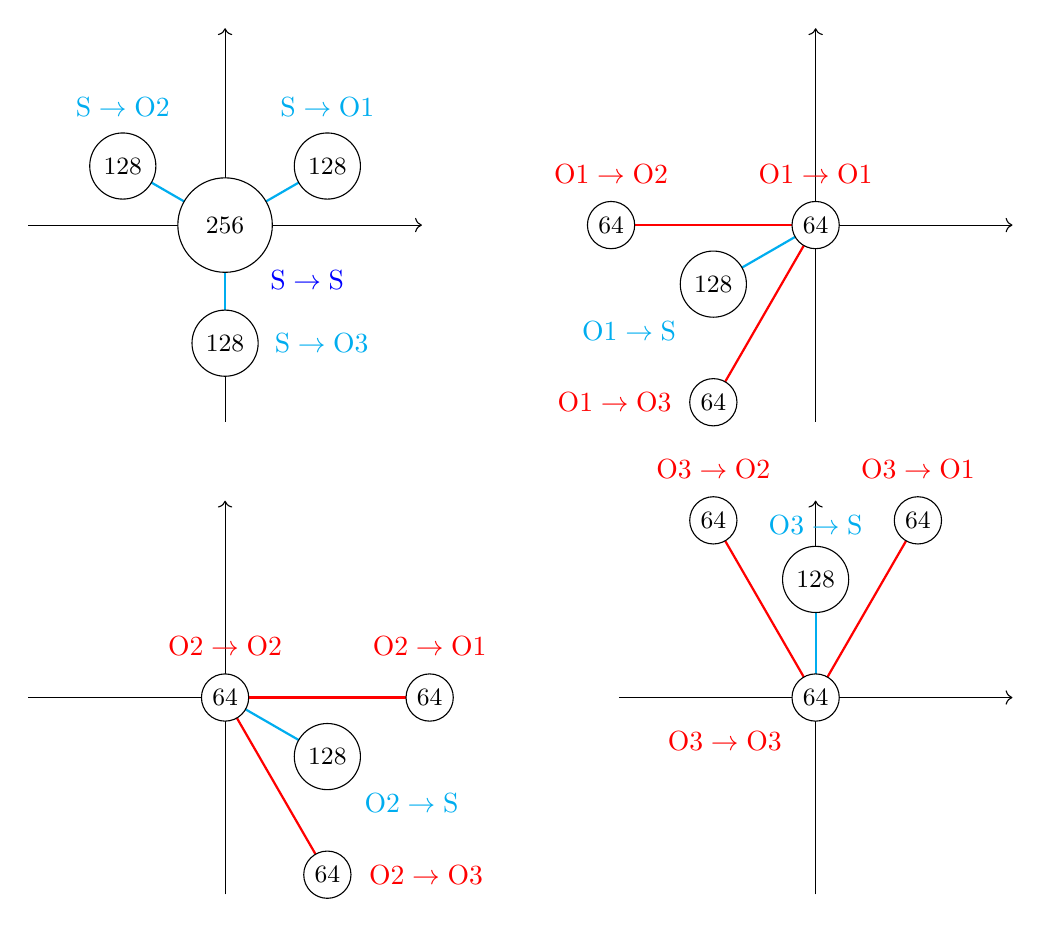
\begin{tikzpicture}
            \draw[->] (-2.5,0)--(2.5,0);
            \draw[->] (0,-2.5)--(0,2.5);
            \draw[cyan,thick] (0,0)--+(30:1.5)node[above=0.5cm]{\(\mathrm{S\to O1}\)};
            \draw[cyan,thick] (0,0)--+(150:1.5)node[above=0.5cm]{\(\mathrm{S\to O2}\)};
            \draw[cyan,thick] (0,0)--+(270:1.5)node[right=0.5cm]{\(\mathrm{S\to O3}\)};
            \node at (0,0)[blue,below right=0.45cm]{\(\mathrm{S\to S}\)};
            \draw[fill=white] (0,0) node{\small\(256\)} circle (0.6);
            \draw[fill=white] (30:1.5) node{\small\(128\)} circle (0.42);
            \draw[fill=white] (150:1.5) node{\small\(128\)} circle (0.42);
            \draw[fill=white] (270:1.5) node{\small\(128\)} circle (0.42);
            \begin{scope}[shift={(7.5,0)}]
                \draw[->] (-2.5,0)--(2.5,0);
                \draw[->] (0,-2.5)--(0,2.5);
                \begin{scope}[shift={(210:1.5)}]
                    \draw[cyan,thick] (0,0)--(30:1.5)node[red,above=0.4cm]{\(\mathrm{O1\to O1}\)};
                    \draw[red,thick] (30:1.5)--(150:1.5)node[above=0.4cm]{\(\mathrm{O1\to O2}\)};
                    \draw[red,thick] (30:1.5)--(270:1.5)node[left=0.4cm]{\(\mathrm{O1\to O3}\)};
                    \node[cyan] at (0,0)[below left=0.35cm]{\(\mathrm{O1\to S}\)};
                    \draw[fill=white] (0,0) node{\small\(128\)} circle (0.42);
                    \draw[fill=white] (30:1.5) node{\small\(64\)} circle (0.3);
                    \draw[fill=white] (150:1.5) node{\small\(64\)} circle (0.3);
                    \draw[fill=white] (270:1.5) node{\small\(64\)} circle (0.3);
                \end{scope}
            \end{scope}
            \begin{scope}[shift={(0,-6)}]
                \draw[->] (-2.5,0)--(2.5,0);
                \draw[->] (0,-2.5)--(0,2.5);
                \begin{scope}[shift={(330:1.5)}]
                    \draw[red,thick] (150:1.5)--(30:1.5)node[above=0.4cm]{\(\mathrm{O2\to O1}\)};
                    \draw[cyan,thick] (0,0)--(150:1.5)node[red,above=0.4cm]{\(\mathrm{O2\to O2}\)};
                    \draw[red,thick] (150:1.5)--(270:1.5)node[right=0.4cm]{\(\mathrm{O2\to O3}\)};
                    \node[cyan] at (0,0)[below right=0.35cm]{\(\mathrm{O2\to S}\)};
                    \draw[fill=white] (0,0) node{\small\(128\)} circle (0.42);
                    \draw[fill=white] (30:1.5) node{\small\(64\)} circle (0.3);
                    \draw[fill=white] (150:1.5) node{\small\(64\)} circle (0.3);
                    \draw[fill=white] (270:1.5) node{\small\(64\)} circle (0.3);
                \end{scope}
            \end{scope}
            \begin{scope}[shift={(7.5,-6)}]
                \draw[->] (-2.5,0)--(2.5,0);
                \draw[->] (0,-2.5)--(0,2.5);
                \begin{scope}[shift={(0,1.5)}]
                    \draw[red,thick] (270:1.5)--(30:1.5)node[above=0.4cm]{\(\mathrm{O3\to O1}\)};
                    \draw[cyan,thick] (0,0)--(270:1.5)node[red,below left=0.3cm]{\(\mathrm{O3\to O3}\)};
                    \draw[red,thick] (150:1.5)node[above=0.4cm]{\(\mathrm{O3\to O2}\)}--(270:1.5);
                    \node[cyan] at (0,0)[above=0.45cm]{\(\mathrm{O3\to S}\)};
                    \draw[fill=white] (0,0) node{\small\(128\)} circle (0.42);
                    \draw[fill=white] (30:1.5) node{\small\(64\)} circle (0.3);
                    \draw[fill=white] (150:1.5) node{\small\(64\)} circle (0.3);
                    \draw[fill=white] (270:1.5) node{\small\(64\)} circle (0.3);
                \end{scope}
            \end{scope}
        \end{tikzpicture}
        \caption{Interatomic vectors of \(\mathrm{SO_3}\).}
    \end{figure}

    To evaluate the Patterson function, we need to find all the interatomic vectors. Let's first consider vectors from the central \(\mathrm{S}\) atom. There will be a self-vector (\(\mathrm{S\to S}\)) at the origin, with weight \(16\times 16=256\), and there will be three \(\mathrm{S\to O}\) vectors arranged symmetrically around origin, with weight \(16\times 8=128\) each. Their distance to the origin is the same as the \(\mathrm{S-O}\) bond length, which we will denote as \(r_1\). Note that this looks like the molecule itself, with the \(\mathrm{S}\) atom sitting at the origin.

    Then consider the vectors from the atom \(\mathrm{O1}\). There will be a self vector (\(\mathrm{O1\to O1}\)) at the origin, with weight \(8\times 8=64\). There are two other \(\mathrm{O\to O}\) vectors, \(\mathrm{O1\to O2}\) and \(\mathrm{O1\to O2}\), at \(60^\circ\) to each other, with weight \(64\) and length \(\sqrt{3}r_1\). Bisecting these two is a \(\mathrm{S\to O1}\) vector with weight \(128\) and length \(r_1\). Note this again look like the molecule itself, but now with \(\mathrm{O1}\) sitting at the origin. Similarly, we can consider vectors from atoms \(\mathrm{O2}\) and \(\mathrm{O3}\) as well.

    Then to construct the Patterson function, we only need to add these contributions up. The result is shown in the figure below.
    \begin{figure}[ht!]
        \centering
        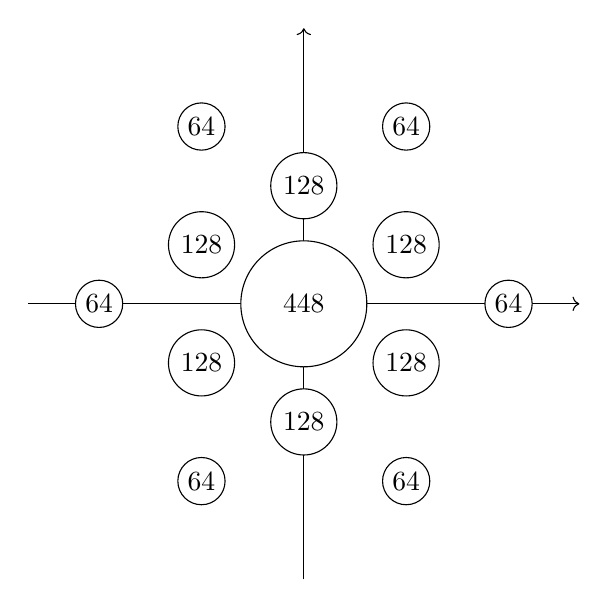
\begin{tikzpicture}
            \draw[->] (-3.5,0)--(3.5,0);
            \draw[->] (0,-3.5)--(0,3.5);
            \draw[fill=white] (0,0)node{448} circle (0.8);
            \foreach \i in {0,...,5}{
                \draw[fill=white] (30+\i*60:1.5) node{128} circle (0.42);
                \draw[fill=white] (\i*60:2.6) node{64} circle (0.3);
            }
        \end{tikzpicture}
        \caption{The Patterson function of a \(\mathrm{SO_3}\) molecule.}
    \end{figure}

    Some remarks:
    \begin{itemize}
        \item The weight of the origin is the sum of the squares the atomic numbers of all atoms.
        \item The Patterson function includes vectors between all atoms, not just between the chemically bonded ones.
        \item \(P(\vb{u})\) must have a centre of symmetry at the origin, even though \(\mathrm{SO_3}\) does not have one. The point group of the \(\mathrm{SO_3}\) molecule is \(D_{3h}\), and the centre of symmetry have upgraded the point group of the Patterson function to \(D_{6h}\).
    \end{itemize}

    One can use the same principle to construct the Patterson of a 3D molecule. Below an example of the Patterson function of \(\mathrm{SO_4^{2-}}\) ion, with \(T_d\) symmetry. The Patterson function has an extra inversion centre, so its point group is \(O_h\).
    \begin{figure}[ht!]
        \centering
        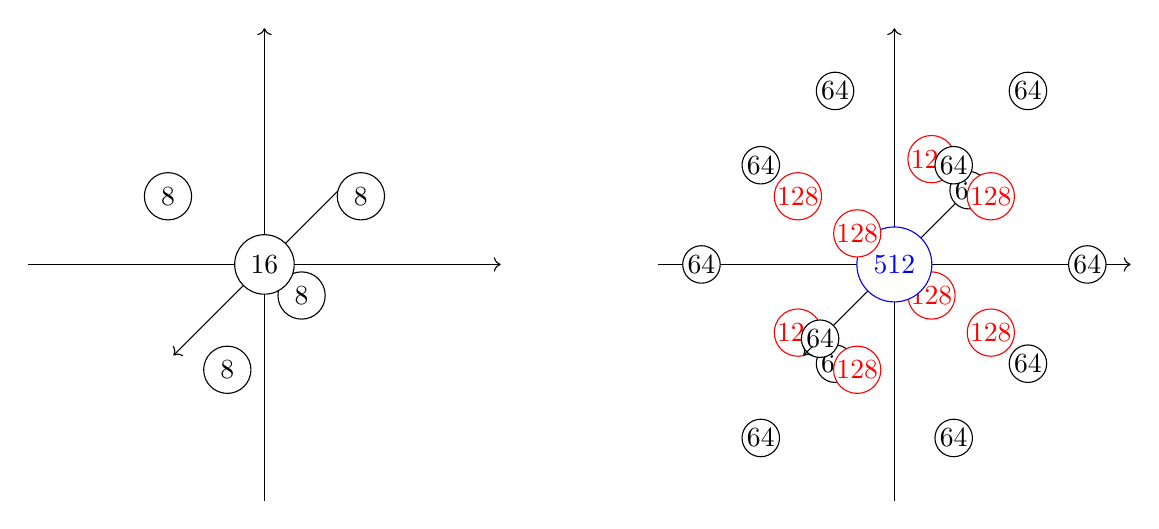
\begin{tikzpicture}
            \draw[->] (0,-3)--(0,3);
            \draw[->] (-3,0)--(3,0);
            \draw[->] (0,0,-3)--(0,0,3);
            \draw[fill=white] (0,-0.866,-1.225) node{8} circle (0.3);
            \draw[fill=white] (0,0,0) node{16} circle (0.378);
            \draw[fill=white] (35.25:1.5) node{8} circle (0.3);
            \draw[fill=white] (144.75:1.5) node{8} circle (0.3);
            \draw[fill=white] (0,-0.866,1.225) node{8} circle (0.3);
            \begin{scope}[shift={(8,0)}]
                \draw[->] (0,-3)--(0,3);
                \draw[->] (-3,0)--(3,0);
                \draw[->] (0,0,-3)--(0,0,3);
                \draw[fill=white] (0,0,-2.45) node{64} circle (0.238);
                \draw[red,fill=white] (0,-0.866,-1.225) node{128} circle (0.3);
                \draw[red,fill=white] (0,0.866,-1.225) node{128} circle (0.3);
                \draw[fill=white] (1.225,1.732,-1.225) node{64} circle (0.238);
                \draw[fill=white] (-1.225,1.732,-1.225) node{64} circle (0.238);
                \draw[fill=white] (1.225,-1.732,-1.225) node{64} circle (0.238);
                \draw[fill=white] (-1.225,-1.732,-1.225) node{64} circle (0.238);
                \draw[blue,fill=white] (0,0,0) node{512} circle (0.476);
                \draw[red,fill=white] (35.25:1.5) node{128} circle (0.3);
                \draw[red,fill=white] (144.75:1.5) node{128} circle (0.3);
                \draw[red,fill=white] (-35.25:1.5) node{128} circle (0.3);
                \draw[red,fill=white] (-144.75:1.5) node{128} circle (0.3);
                \draw[fill=white] (2.45,0) node{64} circle (0.238);
                \draw[fill=white] (-2.45,0) node{64} circle (0.238);
                \draw[red,fill=white] (0,-0.866,1.225) node{128} circle (0.3);
                \draw[red,fill=white] (0,0.866,1.225) node{128} circle (0.3);
                \draw[fill=white] (1.225,1.732,1.225) node{64} circle (0.238);
                \draw[fill=white] (-1.225,1.732,1.225) node{64} circle (0.238);
                \draw[fill=white] (1.225,-1.732,1.225) node{64} circle (0.238);
                \draw[fill=white] (-1.225,-1.732,1.225) node{64} circle (0.238);
                \draw[fill=white] (0,0,2.45) node{64} circle (0.238);
                \draw[->] (0,0,2.688)--(0,0,3);
            \end{scope}
        \end{tikzpicture}
        \caption{The electron density and the Patterson function of \(\mathrm{SO_4^{2-}}\).}
    \end{figure}

    \subsection{The Patterson Function of Ideal Gas}
    We now move on to a more realistic case where there is a whole collection of molecules, and we will consider two extremes --- an ideal gas and a crystalline solid.

    First, let's consider an ideal gas. There are no intermolecular forces, negligible molecular volumes, and we will assume that all molecules are perfectly rigid and geometrically identical. The Patterson peaks will have contribution from all molecules: both intermolecular vectors and intramolecular vectors. For the vectors pointing within a molecule, the interatomic vectors should be identical to that for a single molecule, multiplied by the total number of molecules that are present. But as we are in the gas phase, we have another complexity. Due to the random molecular orientation, the Patterson function of an ideal gas appears as a spherically averaged version of the 3D Patterson that we constructed for one molecule. Thus, only the length of the interatomic vector is important, and we will plot the resulting Patterson function as a radial vector map. For example, for the \(\mathrm{SO_4^{2-}}\) ideal gas (which apparently will not be ideal in reality), the radial Patterson function is shown in the figure below.\footnote{As for the atomic wavefunction, you can choose to plot a radial Patterson function or a radial distribution function --- we are being rather loose here since we are doing everything schematically. Anyway, the true weight of a peak is the integral of the 3D Patterson function.}
    \begin{figure}[ht!]
        \centering
        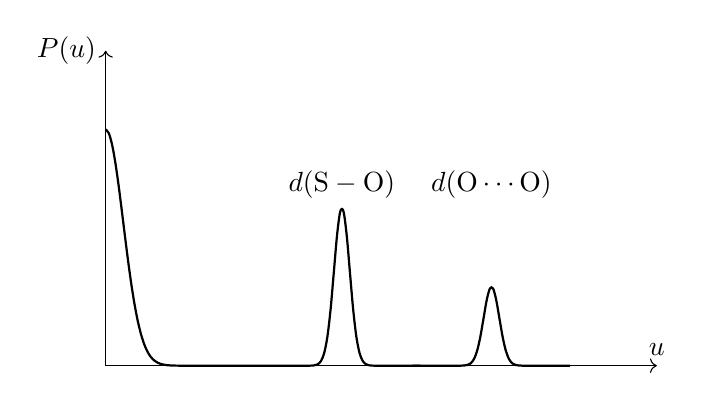
\begin{tikzpicture}
            \draw[->] (0,0)--(7,0)node[above]{\(u\)};
            \draw[->] (0,0)--(0,4)node[left]{\(P(u)\)};
            \draw[thick,domain=0:2, smooth, variable=\x,samples=50] plot ({\x}, {3*2.72^(-10*\x*\x)});
            \draw[thick,domain=-1:1, smooth, variable=\x,samples=50] plot ({\x+3}, {2*2.72^(-50*\x*\x)});
            \draw[thick,domain=-1:1, smooth, variable=\x,samples=50] plot ({\x+4.9}, {1*2.72^(-50*\x*\x)});
            \node at (3,2)[above]{\(d(\mathrm{S-O})\)};
            \node at (4.9,2)[above]{\(d(\mathrm{O\cdots O})\)};
        \end{tikzpicture}
        \caption{Intramolecular contribution to the radial Patterson function of \(\mathrm{SO_4^{2-}}\).}
    \end{figure}

    We then need to consider the intermolecular vectors. If the gas is indeed ideal with no intermolecular forces, then the positions and orientations of all molecules should be completely random at any time. Hence, all distances between molecules are equally possible, and so the intermolecular vectors will sum over time to form a constant background. If we are going to inject a little bit of reality into this crude model, we can say that the molecules cannot be too close from each other, so this background is zero at small \(u\).

    \begin{figure}[ht!]
        \centering
        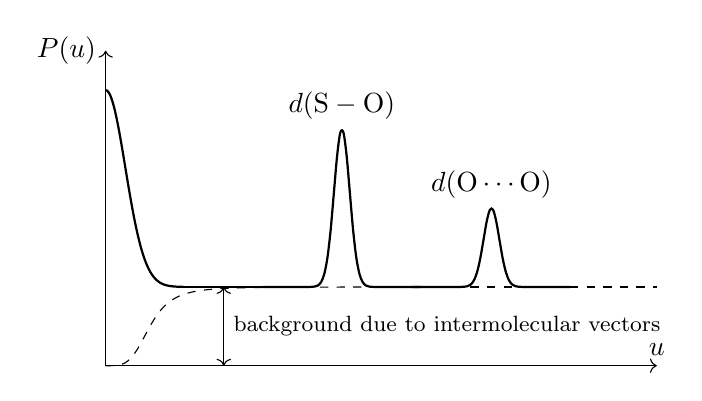
\begin{tikzpicture}
            \draw[->] (0,0)--(7,0)node[above]{\(u\)};
            \draw[->] (0,0)--(0,4)node[left]{\(P(u)\)};
            \draw[thick,domain=0:1, smooth, variable=\x,samples=50] plot ({\x}, {2.5*2.72^(-8*\x*\x)+1});
            \draw[thick,domain=-1:1, smooth, variable=\x,samples=50] plot ({\x+3}, {2*2.72^(-50*\x*\x)+1});
            \draw[thick,domain=-1:1, smooth, variable=\x,samples=50] plot ({\x+4.9}, {1*2.72^(-50*\x*\x)+1});
            \draw[dashed, domain=0:4, smooth, variable=\x,samples=50] plot ({\x}, {10*\x*\x*\x*\x/(1+10*\x*\x*\x*\x)});
            \node at (3,3)[above]{\(d(\mathrm{S-O})\)};
            \node at (4.9,2)[above]{\(d(\mathrm{O\cdots O})\)};
            \draw[thick] (1,1)--(2,1);
            \draw[dashed] (4,1)--(7,1);
            \draw[<->] (1.5,0)--node[right]{\footnotesize background due to intermolecular vectors}(1.5,1);
        \end{tikzpicture}
        \caption{Radial Patterson function of \(\mathrm{SO_4^{2-}}\) with both intermolecular and intramolecular contributions.}
    \end{figure}

    As a result, in an ideal gas, the radial Patterson function has discernible peaks corresponding solely to the spherically averaged Patterson function of one molecule, superimposed on a featureless background. Non-ideal gases, liquid and non-crystalline solid will show similar radial Patterson function due their disorderedness. However, they may show local coordination peaks.

    \newpage
    \section{Diffraction from a Single Crystal}
    In the remainder of the course, we will focus almost exclusively on single crystals, since as we will see, we can develop robust methods to interpret single-crystal diffraction patterns.
    \subsection{Diffracted Intensity for a Single Crystal}
    We will first infer how the Patterson function of a crystal would look like --- this shouldn't be too difficult due to the order in a crystal, and then we will perform the Fourier transform to try to figure out the form of its diffracted intensity.

    We will consider a single crystal with unit cell vectors \(\vb{a},\vb{b},\vb{c}\), with \(N=N_a\times N_b\times N_c\) unit cells in total, where \(N_a,N_b,N_c\) are the number of cells along each direction.

    Suppose the Patterson function of a single unit cell is \(P_{\text{cell}}(\vb{u})\), then its Fourier transform will give the diffracted intensity from one unit cell, which we will call \(\abs{F_{\text{cell}}(\vb{S})}^2\).
    \begin{equation}
        \abs{F_{\text{cell}}}^2=\int\dd[3]{\vb{u}}\ee^{2\pi \ii\vb{u}\vdot\vb{S}}P_{\text{cell}}(\vb{u})\,.
    \end{equation}
    Then for our single crystal, there will be \(N\) such contributions to the diffracted intensities, so we get the intra-cell contribution \(N \abs{F_{\text{cell}}(\vb{S})}^2\).

    Next consider the contribution to the Patterson function by inter-cell vectors pointing from each cell to the cell next to it along the \(+\vb{a}\) direction. For each intra-cell vector \(\vb{u}\), there must be such a inter-cell vector \(\vb{u}+\vb{a}\), so the contribution to the Patterson function from this type of inter-cell vectors is \(P_{\text{cell}}(\vb{u}+\vb{a})\). This contributes
    \begin{equation}
        \int\dd[3]{\vb{u}}P_{\text{cell}}(\vb{u}+\vb{a})\ee^{2\pi \ii\vb{u}\vdot\vb{S}}
    \end{equation}
    to the diffraction intensity. We can simplify this a bit further. By the change of variable \(\vb{v}=\vb{u}+\vb{a}\), we have
    \begin{align}
        \int\dd[3]{\vb{u}}P_{\text{cell}}(\vb{u}+\vb{a})\ee^{2\pi \ii\vb{u}\vdot\vb{S}}&=\int\dd[3]{\vb{v}}P_{\text{cell}}(\vb{v})\ee^{2\pi \ii\vb{v}\vdot\vb{S}}\ee^{-2\pi \ii\vb{a}\vdot\vb{S}}\notag \\
        &=\abs{F_{\text{cell}}}^2 \ee^{-2\pi \ii\vb{a}\vdot\vb{S}}\,.
    \end{align}
    However, there are only \((N_a-1)N_bN_c\) cells have such a neighbouring cell one unit along \(+\vb{a}\) direction, so its contribution to the diffraction intensity is
    \begin{equation}
        (N_a-1)N_bN_c\abs{F_{\text{cell}}}^2 \ee^{-2\pi \ii\vb{a}\vdot\vb{S}}\,.
    \end{equation}
    Similarly, there are also contributions from inter-cell vectors pointing from a cell to the neighbouring cell along \(-\vb{a}\) direction, which is
    \begin{equation}
        (N_a-1)N_bN_c\abs{F_{\text{cell}}}^2 \ee^{+2\pi \ii\vb{a}\vdot\vb{S}}\,.
    \end{equation}

    The rest of the process is similar, there will be inter-cell vectors pointing from one cell to the cell \(n_a\vb{a}+n_b\vb{b}+n_c\vb{c}\) away for any \(-N_a< n_a< N_a\), \(-N_b< n_b< N_b\), \(-N_c< n_c< N_c\), contributing
    \begin{equation}
        (N_a-\abs{n_a})(N_b-\abs{n_b})(N_c-\abs{n_c})\abs{F_{\text{cell}}}^2 \ee^{-2\pi \ii(n_a\vb{a}+n_b\vb{b}+n_c\vb{c})\vdot\vb{S}}
    \end{equation}
    to the total diffraction intensity. We need to sum all of these up, and we get a total diffraction intensity
    \begin{align}
        I(\vb{S})&=\abs{F_{\text{cell}}}^2\sum_{n_a=-N_a}^{N_a}\sum_{n_b=-N_b}^{N_b}\sum_{n_c=-N_c}^{N_c}(N_a-\abs{n_a})(N_b-\abs{n_b})(N_c-\abs{n_c})\ee^{-2\pi \ii(n_a\vb{a}+n_b\vb{b}+n_c\vb{c})\vdot\vb{S}}\notag \\
        &=\abs{F_{\text{cell}}}^2\prod_{j\in\{a,b,c\}}\sum_{n_j=-N_j+1}^{N_j-1}(N_j-\abs{n_j})\ee^{-2\pi \ii n_j\vb{j}\vdot\vb{S}}\,.
    \end{align}
    The latter form is rather more compact, but less intuitive.\footnote{You might have noticed that the limits of the sum should be \(\pm(N_j-1)\) instead of \(N_j\). We have included \(n_j=\pm N_j\) into our sum since they contribute nothing and can make our formula slightly more compact.}

    \subsubsection*{A more Mathematical View}
    Consider the convolution of some function \(f(\vb{r})\) with a Dirac delta \(\delta(\vb{r}-\vb{a})\) with its peak at \(\vb{r}=\vb{a}\).
    \begin{equation}
        f(\vb{r})*\delta(\vb{r}-\vb{a})=\int_{-\infty}^{\infty}\dd[3]{\vb{u}}f(\vb{u})\delta(\vb{u}-(\vb{r}-\vb{a}))=f(\vb{r}-\vb{a})\,.
    \end{equation}
    We see that its effect is to shift \(f(\vb{r})\) by \(\vb{a}\) --- or in other words, it put a copy of \(f(\vb{r})\) at position \(\vb{a}\). A crystal is essentially a copy of \(\rho_{\text{cell}}\) at each lattice point\footnote{This is not quite accurate as a unit cell may contain more than one lattice point in non-primitive cell. This is not a crystallographic course so we will be rather loose here.}. This allows us to view the electron density of a crystal as the convolution of the lattice of Dirac delta functions with the electron density of a single unit cell:
    \begin{equation}\label{crystal_electron_density_as_convolution}
        \rho(\vb{r})=\rho_{\text{cell}}(\vb{r})*\rho_{\text{lattice}}(\vb{r})\,,
    \end{equation}
    where
    \begin{equation}
        \rho_{\text{lattice}}(\vb{r})=\sum_{n_a=0}^{N_a-1}\sum_{n_b=0}^{N_b-1}\sum_{n_c=0}^{N_c-1}\delta(\vb{r}-n_a\vb{a}-n_b\vb{b}-n_c\vb{c})
    \end{equation}
    is the lattice of delta functions (It is obviously not a electron density, but we will denote it as \(\rho\) anyway). A rather useful properties is the Patterson function of a convolution is the convolution of the Patterson functions,\footnote{This is perhaps not too obvious to prove using the integral definitions of these quantities. However, an important fact of electron density is that it is a real function, so \(P(\vb{r})=\rho(\vb{r})\otimes\rho(\vb{r})=\rho(\vb{r})*\rho(-\vb{r})\). Then
    \begin{align}
        P(\vb{r})&=\rho(\vb{r})*\rho(-\vb{r})\notag \\
        &=[\rho_{\text{cell}}(\vb{r})*\rho_{\text{lattice}}(\vb{r})]*[\rho_{\text{cell}}(-\vb{r})*\rho_{\text{lattice}}(-\vb{r})]\notag \\
        &=[\rho_{\text{cell}}(\vb{r})*\rho_{\text{cell}}(-\vb{r})]*[\rho_{\text{lattice}}(\vb{r})*\rho_{\text{lattice}}(-\vb{r})]\notag \\
        &=P_{\text{cell}}(\vb{r})*P_{\text{lattice}}(\vb{r})
    \end{align}
    by the commutativity and associativity of convolution (which are not that difficult to prove).} and so
    \begin{equation}
        P(\vb{u})=P_{\text{cell}}(\vb{u})*P_{\text{lattice}}(\vb{u})\,.
    \end{equation}
    The Patterson function (autocorrelation) of the lattice of delta functions is
    \begin{equation}
        P_{\text{lattice}}(\vb{u})=\sum_{n_a=-N_a}^{N_a}\sum_{n_b=-N_b}^{N_b}\sum_{n_c=-N_c}^{N_c}(N_a-\abs{n_a})(N_b-\abs{n_b})(N_c-\abs{n_c})\delta(\vb{u}-n_a\vb{a}-n_b\vb{b}-n_c\vb{c})\,.
    \end{equation}
    Then by the convolution theorem, the diffracted intensity, which is the Fourier transform of the Patterson function, must be the product of the diffracted intensity of a unit cell \(\abs{F_{\text{cell}}(\vb{r})}^2\) with the Fourier transform of this Patterson function of the lattice, which is given by
    \begin{equation}
        I(\vb{S})=\abs{F_{\text{cell}}}^2\sum_{n_a=-N_a}^{N_a}\sum_{n_b=-N_b}^{N_b}\sum_{n_c=-N_c}^{N_c}(N_a-\abs{n_a})(N_b-\abs{n_b})(N_c-\abs{n_c})\ee^{-2\pi \ii(n_a\vb{a}+n_b\vb{b}+n_c\vb{c})\vdot\vb{S}}\,.
    \end{equation}
    We have arrived at the same result.

    \subsection{The Reciprocal Lattice}
    Although we can't measure the structure factor, we can still work it out assuming we know \(\rho(\vb{r})\) to see how it looks like for a single crystal. Using the above expression of the electron density as a convolution (\ref{crystal_electron_density_as_convolution}), we can directly take its Fourier transform and get the structure factor
    \begin{align}
        F(\vb{S})&=F_{\text{cell}}(\vb{S})\mathcal{F}\left[\sum_{n_a=0}^{N_a-1}\sum_{n_b=0}^{N_b-1}\sum_{n_c=0}^{N_c-1}\delta(\vb{r}-n_a\vb{a}-n_b\vb{b}-n_c\vb{c})\right]\notag \\
        &=F_{\text{cell}}(\vb{S})\left[\sum_{n_a=0}^{N_a-1}\sum_{n_b=0}^{N_b-1}\sum_{n_c=0}^{N_c-1}\ee^{-2\pi \ii(n_a\vb{a}+n_b\vb{b}+n_c\vb{c})\vdot\vb{S}}\right]\notag \\
        &=F_{\text{cell}}(\vb{S})\prod_{j\in\{a,b,c\}}\sum_{n_j=0}^{N_j-1}\ee^{-2\pi \ii n_j\vb{j}\vdot\vb{S}}\,.
    \end{align}
    We see a cute geometric series here! This allows to simplify it further
    \begin{align}
        F(\vb{S})&=F_{\text{cell}}(\vb{S})\prod_{j\in\{a,b,c\}}\frac{1-\exp[-2\pi \ii N_j\vb{j}\vdot\vb{S}]}{1-\exp[-2\pi \ii\vb{j}\vdot\vb{S}]}\notag \\
        &=F_{\text{cell}}(\vb{S})\prod_{j\in\{a,b,c\}}\frac{\exp[-\pi \ii N_j\vb{j}\vdot\vb{S}]}{\exp[-\pi \ii\vb{j}\vdot\vb{S}]}\frac{\exp[\pi \ii N_j\vb{j}\vdot\vb{S}]-\exp[-\pi \ii N_j\vb{j}\vdot\vb{S}]}{\exp[\pi \ii\vb{j}\vdot\vb{S}]-\exp[-\pi \ii\vb{j}\vdot\vb{S}]}\notag \\
        &=F_{\text{cell}}(\vb{S})\prod_{j\in\{a,b,c\}}\exp[-\pi \ii (N_j-1)\vb{j}\vdot\vb{S}]\frac{\sin(\pi N_j\vb{j}\vdot\vb{S})}{\sin(\pi\vb{j}\vdot\vb{S})}
    \end{align}
    Having the structure factor in this form, we can work out another expression of the diffraction intensity of single crystal
    \begin{align}
        I(\vb{S})&=F(\vb{S})F^*(\vb{S})\notag\\
        &=\abs{F_{\text{cell}}(\vb{S})}^2\prod_{j\in\{a,b,c\}}\frac{\sin^2(\pi N_j\vb{j}\vdot\vb{S})}{\sin^2(\pi\vb{j}\vdot\vb{S})}\notag\\
        &=\abs{F_{\text{cell}}(\vb{S})}^2\frac{\sin^2(\pi N_a\vb{a}\vdot\vb{S})}{\sin^2(\pi\vb{a}\vdot\vb{S})}\frac{\sin^2(\pi N_b\vb{b}\vdot\vb{S})}{\sin^2(\pi\vb{b}\vdot\vb{S})}\frac{\sin^2(\pi N_c\vb{c}\vdot\vb{S})}{\sin^2(\pi\vb{c}\vdot\vb{S})}\,.
    \end{align}
    This is somewhat easier to plot. To make the plotting easier, we will consider a 1D crystal of \(N\) units cell, so
    \begin{equation}
        \frac{I(S)}{\abs{F_{\text{cell}}(S)}^2}=\frac{\sin^2(\pi NaS)}{\sin^2(\pi aS)}\,.
    \end{equation}
    Let's plot this function at different values of \(N\) and see how they look like.

    \begin{figure}[ht!]
        \centering
        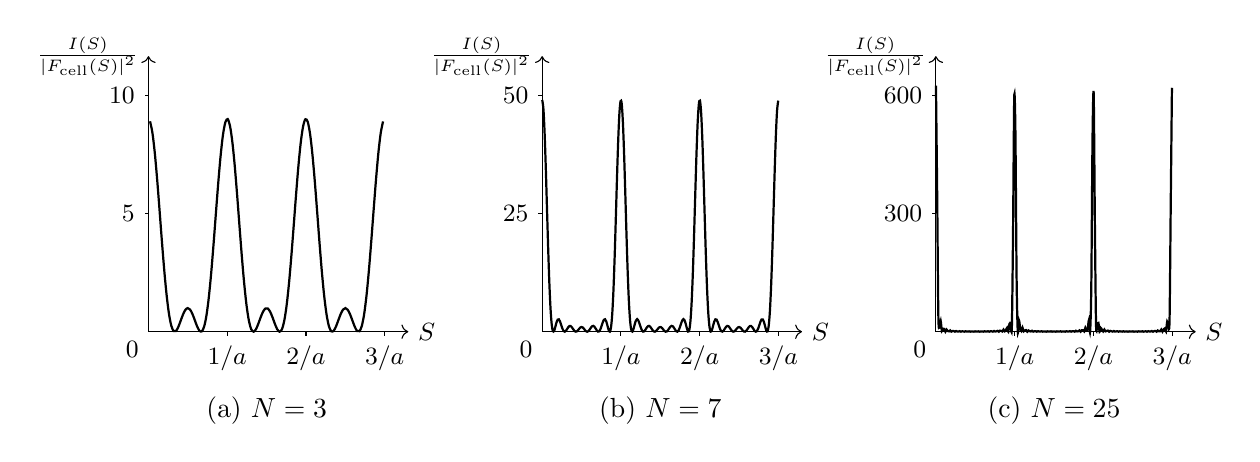
\begin{tikzpicture}
            \draw[->] (0,0)node[below left]{\small 0}--(3.3,0)node[right]{\small\(S\)};
            \draw[->] (0,0)--(0,3.5)node[left]{\small\(\frac{I(S)}{\abs{F_{\text{cell}}(S)}^2}\)};
            \draw (1,0)--(1,-0.05)node[below]{\small\(1/a\)};
            \draw (2,0)--(2,-0.05)node[below]{\small\(2/a\)};
            \draw (3,0)--(3,-0.05)node[below]{\small\(3/a\)};
            \draw (0,1.5)--(-0.05,1.5)node[left]{\small\(5\)};
            \draw (0,3)--(-0.05,3)node[left]{\small\(10\)};
            \draw[thick,domain=0.02:2.98, smooth, variable=\x,samples=100] plot ({\x}, {0.3*(sin(3.1415*3*\x r)/sin(3.1415*\x r))^2});
            \node at (1.5,-1){(a) \(N=3\)};
            \begin{scope}[shift={(5,0)}]
                \draw[->] (0,0)node[below left]{\small 0}--(3.3,0)node[right]{\small\(S\)};
                \draw[->] (0,0)--(0,3.5)node[left]{\small\(\frac{I(S)}{\abs{F_{\text{cell}}(S)}^2}\)};
                \draw (1,0)--(1,-0.05)node[below]{\small\(1/a\)};
                \draw (2,0)--(2,-0.05)node[below]{\small\(2/a\)};
                \draw (3,0)--(3,-0.05)node[below]{\small\(3/a\)};
                \draw (0,1.5)--(-0.05,1.5)node[left]{\small\(25\)};
                \draw (0,3)--(-0.05,3)node[left]{\small\(50\)};
                \draw[thick,domain=0.001:2.999, smooth, variable=\x,samples=200] plot ({\x}, {0.06*(sin(3.1415*7*\x r)/sin(3.1415*\x r))^2});
                \node at (1.5,-1){(b) \(N=7\)};
            \end{scope}
            \begin{scope}[shift={(10,0)}]
                \draw[->] (0,0)node[below left]{\small 0}--(3.3,0)node[right]{\small\(S\)};
                \draw[->] (0,0)--(0,3.5)node[left]{\small\(\frac{I(S)}{\abs{F_{\text{cell}}(S)}^2}\)};
                \draw[thick,domain=0.001:2.999, smooth, variable=\x,samples=200] plot ({\x}, {0.005*(sin(3.1415*25*\x r)/sin(3.1415*\x r))^2});
                \draw (0,1.5)--(-0.05,1.5)node[left]{\small\(300\)};
                \draw (0,3)--(-0.05,3)node[left]{\small\(600\)};
                \draw (1,0)--(1,-0.05)node[below]{\small\(1/a\)};
                \draw (2,0)--(2,-0.05)node[below]{\small\(2/a\)};
                \draw (3,0)--(3,-0.05)node[below]{\small\(3/a\)};
                \node at (1.5,-1){(c) \(N=25\)};
            \end{scope}
        \end{tikzpicture}
    \end{figure}

    We see that the functions have principal maxima at \(S=k/a\) for integer values of \(k\), and there are \(N-2\) subsidiary maxima between the principal maxima. As we increase \(N\), the principal maxima becomes too strong that we can no longer see the subsidiary maxima. We can see this by taking the limit
    \begin{equation}
        \lim_{S\to k/a}\frac{\sin^2(\pi NaS)}{\sin^2(\pi aS)}=\lim_{u\to k}\left(\frac{\sin Nu\pi}{\sin u\pi}\right)^2=\lim_{u\to k}\left(\frac{N\pi\cos Nu\pi}{\pi\cos u\pi}\right)^2=N^2\,,
    \end{equation}
    so the height of the principal maxima is \(N^2\). Hence, in the limit of large \(N\) (in real-life crystals, \(N\sim 10^{23}\)), we can well-approximate the diffraction pattern of single crystals as discrete beams, separated by \(1/a\).

    Similarly, in a 3D crystals, the diffraction intensity will only be observable at discrete values of \(\vb{S}\) separated by \(1/\norm{\vb{a}}\), \(1/\norm{\vb{b}}\) and \(1/\norm{\vb{c}}\). This forms what is called a \textit{reciprocal lattice}, with lattice vectors \(\vb{a}^*\), \(\vb{b}^*\) and \(\vb{c}^*\) given by
    \begin{align}
        \vb{a}^*&=\frac{\vb{b}\cross\vb{c}}{V} & \vb{b}^*&=\frac{\vb{c}\cross\vb{a}}{V} & \vb{c}^*&=\frac{\vb{a}\cross\vb{b}}{V}\,,
    \end{align}
    where \(V=\vb{a}\vdot(\vb{b}\cross\vb{c})\) is the volume of the unit cell. We will only observe diffracted beams with
    \begin{equation}
        \vb{S}=h\vb{a}^*+k\vb{b}^*+l\vb{c}^*\,,
    \end{equation}
    i.e. on the reciprocal lattice points. We will show later that this corresponds to the same \(h,k,l\) as in the Miller planes in Bragg's description of diffraction which you might have seen if you take Part IA Material Sciences.

    It is called the reciprocal lattice because it lives in the reciprocal space (Fourier domain). In fact, the reciprocal lattice is the Fourier transform of the real lattice. The unit of the reciprocal lattice vectors are \(\text{length}^{-1}\), and their magnitudes are given by
    \begin{align}
        \norm{\vb{a}^*}&=\frac{\norm{\vb{b}}\norm{\vb{c}}\sin\alpha}{V} & \norm{\vb{b}^*}&=\frac{\norm{\vb{c}}\norm{\vb{a}}\sin\beta}{V} & \norm{\vb{c}^*}&=\frac{\norm{\vb{a}}\norm{\vb{b}}\sin\gamma}{V}\,,
    \end{align}
    where \(\alpha\) is the angle between \(\vb{b}\) and \(\vb{c}\), \textit{etc.} This means that we can view the reciprocal lattice as ``the lattice of periodicities in a crystal''. To see this, let's consider all the possible set of repeated parallel planes that are compatible with the periodicity of the crystal. By being compatible with the periodicity, we require it to look identical in different unit cells, which requires the planes to intersect each edge of the lattice an integer number of times. This allows us to define the \textit{Miller indices} for repeated planes in crystals by specifying how many times the plane intersect with the edge of the cell in each direction. If we put the first plane at the origin and the second plane intersects the axes at \(1/h\), \(1/k\) and \(1/l\) for \(h,k,l\in\mathbb{Z}\), then we would label these planes as \((hkl)\). Then this set of planes will intersect \(\vb{a}\) axis \(h\) times, \(\vb{b}\) axis \(k\) times and \(\vb{c}\) axis \(l\) times.

    \begin{figure}[ht!]
        \centering
        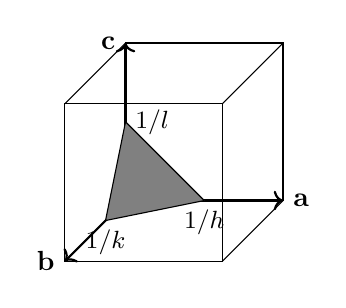
\begin{tikzpicture}
            \draw (0,0,0) rectangle (2,2,0);
            \draw (0,0,2) rectangle (2,2,2);
            \draw (0,0,0)--(0,0,2);
            \draw (2,0,0)--(2,0,2);
            \draw (0,2,0)--(0,2,2);
            \draw (2,2,0)--(2,2,2);
            \draw[->,thick] (0,0,0)--(2,0,0)node[right]{\(\vb{a}\)};
            \draw[->,thick] (0,0,0)--(0,0,2)node[left]{\(\vb{b}\)};
            \draw[->,thick] (0,0,0)--(0,2,0)node[left]{\(\vb{c}\)};
            \draw[fill=gray] (1,0,0)node[below]{\small\(1/h\)}--(0,0,0.66)node[below]{\small\(1/k\)}--(0,1,0)node[right]{\small\(1/l\)}--(1,0,0);
        \end{tikzpicture}
        \caption{A \((hkl)\) plane in a unit cell. There will be another \(\max(h,k,l)\) planes parallel to this in this cell, intersecting \(\vb{a}\) axis at \(1/h,2/h,\dots,1\), \(\vb{b}\) axis at \(1/k,2/k,\dots,1\) and \(\vb{c}\) axis at \(1/l,2/l,\dots,1\).}
    \end{figure}

    We can use these planes to construct the reciprocal lattice. Consider viewing the lattice along the \(\vb{b}\) direction, and constructing planes of \((h0l)\) types. For each set of plane, if we draw a vector perpendicular to these planes and magnitude inversely proportional to the interplanar spacing, then the end of these vectors will form the \((h0l)\) section of the reciprocal lattice.

    \begin{figure}
        \centering
        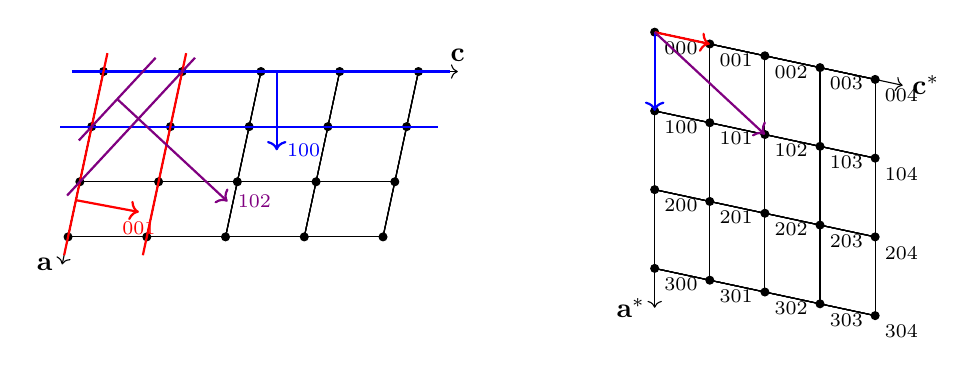
\begin{tikzpicture}
            \foreach \i in {0,...,4}{
                \foreach \j in {0,...,3}{
                    \draw[fill=black] (\i-0.15*\j,-0.7*\j) circle (0.05);
                    \draw (\i,0)--(\i-0.45,-2.1);
                    \draw (-0.15*\j,-0.7*\j)--(4-0.15*\j,-0.7*\j);
                }
            }
            \draw[->] (0,0)--(-0.525,-2.45)node[left]{\(\vb{a}\)};
            \draw[->] (0,0)--(4.5,0)node[above]{\(\vb{c}\)};
            \draw[thick,blue] (-0.4,0)--(4.4,0);
            \draw[thick,blue] (-0.55,-0.7)--(4.25,-0.7);
            \draw[thick,blue,->] (2.2,0)--(2.2,-1)node[right]{\scriptsize\(100\)};
            \draw[thick,red] (0.05,0.2333)--(-0.5,-2.3333);
            \draw[thick,red] (1.05,0.2333)--(0.5,-2.3333);
            \draw[thick,red,->] (-0.35,-1.6333)--(0.45,-1.7833)node[below]{\scriptsize\(001\)};
            \draw[thick,violet] (0.6625,0.175)--(-0.3125,-0.875);
            \draw[thick,violet] (1.1625,0.175)--(-0.4625,-1.575);
            \draw[thick,violet,->] (0.175,-0.35)--+(1.4,-1.3)node[right]{\scriptsize\(102\)};
            \begin{scope}[shift={(7,0.5)}]
                \foreach \i in {0,...,4}{
                    \foreach \j in {0,...,3}{
                        \draw[fill=black] (0.7*\i,-0.15*\i-\j) node[below right]{\scriptsize\(\j 0 \i\)} circle (0.05);
                        \draw (0,-\j)--(2.8,-0.6-\j);
                        \draw (0.7*\i,-0.15*\i)--(0.7*\i,-3-0.15*\i);
                    }
                }
                \draw[->] (0,0)--(3.15,-0.675)node[right]{\(\vb{c}^*\)};
                \draw[->] (0,0)--(0,-3.5)node[left]{\(\vb{a}^*\)};
                \draw[red,thick,->] (0,0)--(0.7,-0.15);
                \draw[blue,thick,->] (0,0)--(0,-1);
                \draw[violet,thick,->] (0,0)--(1.4,-1.3);
            \end{scope}
        \end{tikzpicture}
        \caption{Constructing the reciprocal lattice using planes.}
    \end{figure}

    By the definition of the reciprocal lattice vectors, it is easy to see that
    \begin{equation}
        \vb{i}\vdot\vb{j}^*=\delta_{ij}\,,
    \end{equation}
    \(i,j\in\{a,b,c\}\). Hence, by expanding \(\vb{r}=x\vb{a}+y\vb{b}+z\vb{c}\) and \(\vb{S}=h\vb{a}^*+k\vb{b}^*+l\vb{c}^*\), we can see that
    \begin{align}
        \vb{r}\vdot\vb{S}&=xh\vb{a}\vdot\vb{a}^*+xk\cancel{\vb{a}\vdot\vb{b}^*}+xl\cancel{\vb{a}\vdot\vb{c}^*}\notag\\
        &\quad\ yh\cancel{\vb{b}\vdot\vb{a}^*}+yk\vb{b}\vdot\vb{b}^*+yl\cancel{\vb{b}\vdot\vb{c}^*}\notag\\
        &\quad\ zh\cancel{\vb{c}\vdot\vb{a}^*}+zk\cancel{\vb{c}\vdot\vb{b}^*}+zl\vb{c}\vdot\vb{c}^*\notag\\
        &=xh+yk+zl\,.
    \end{align}
    Therefore for a single crystal, the structure factor can be rewritten as
    \begin{align}
        F(h,k,l)=\int\dd{x}\dd{y}\dd{z}\rho(x,y,z)\ee^{2\pi \ii(hx+ky+lz)}\,.
    \end{align}

    \subsection{Bragg's Law}
    \begin{figure}
        \centering
        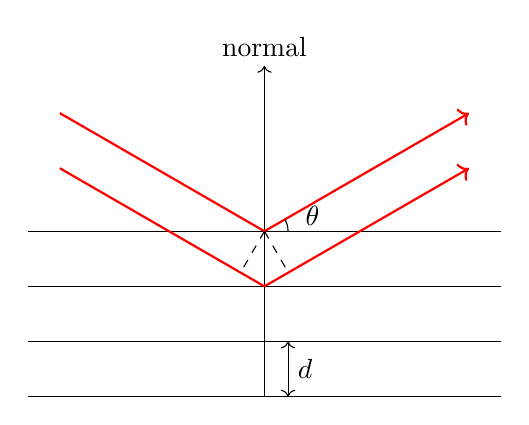
\begin{tikzpicture}
            \foreach \i in {0,...,-3}{
                \draw (-3,0.7*\i)--(3,0.7*\i);
            }
            \draw[->] (0,-2.1)--(0,2.1)node[above]{normal};
            \draw[<->] (0.3,-2.1)--node[right]{\(d\)}(0.3,-1.4);
            \draw[->,red,thick] (0,0)--+(30:3);
            \draw[red,thick] (0,0)--+(150:3);
            \draw[->,red,thick] (0,-0.7)--+(30:3);
            \draw[red,thick] (0,-0.7)--+(150:3);
            \draw (0.3,0) arc (0:30:0.3);
            \node at (0.4,0.2)[right]{\(\theta\)};
            \draw[dashed] (0,0)--+(-60:0.606);
            \draw[dashed] (0,0)--+(-120:0.606);
        \end{tikzpicture}
        \caption{Diffraction using Bragg planes.}
    \end{figure}
    Here we present an alternative view of diffraction in a single crystal, which might be familiar from Part IA Material Sciences. We can think of the diffracted beam as being reflected by the planes in crystals, which are known as the Bragg's planes. The scattering vector is bisecting the incoming and outgoing rays, so it is perpendicular to those imaginary mirror planes. Now for a constructive interference to occur, we need the path difference of light reflected by consecutive Bragg planes to be an integer multiple of the wavelength, so
    \begin{equation}
        n\lambda=2d\sin\theta\,,
    \end{equation} 
    where \(\theta\) is the angle between the planes and the beams, and \(d\) is the interplanar spacing. This factor of \(n\) can be omitted since diffraction from with \(n>1\) from a set of planes \((h\, k\, l)\) with spacing \(d\) is equivalent to diffraction with \(n=1\) from planes with spacing \(d/n\), so we can instead think of them as being reflected from a high-order plane \((nh\, nk\, nl)\). For example, a \(n=4\) reflection from \(100\) planes is equivalent to a \(n=1\) reflection from \(400\) planes. Therefore, we have the Bragg's law
    \begin{equation}
        \lambda=2d\sin\theta
    \end{equation}
    for diffraction to be observed. We have defined \(\norm{\vb{S}}=2\sin\theta/\lambda\), and so \(\norm{\vb{S}}=1/d\). This again shows why diffraction is only observed on reciprocal lattice points.

    \subsection{Practical Measurements of Single-Crystal X-Ray Diffraction}
    Suppose we are measuring the diffraction from a particular single crystal. Since a crystal has a defined orientation, a certain scattering vector \(\vb{S}=h\vb{a}^*+k\vb{b}^*+l\vb{c}^*\) will appear in a well-defined direction relative to the crystal (perpendicular to the \(hkl\) planes). We can think the reciprocal lattice is attached to the crystal, and hence to measure a particular \(hkl\) diffraction, we need to arrange the incident beam to a particular direction relative to the crystal given by the Bragg's law. This requires us to be able to flexibly adjust the relative orientation of the incident beam, the detector and the crystal.
    \begin{figure}[ht!]
        \centering
        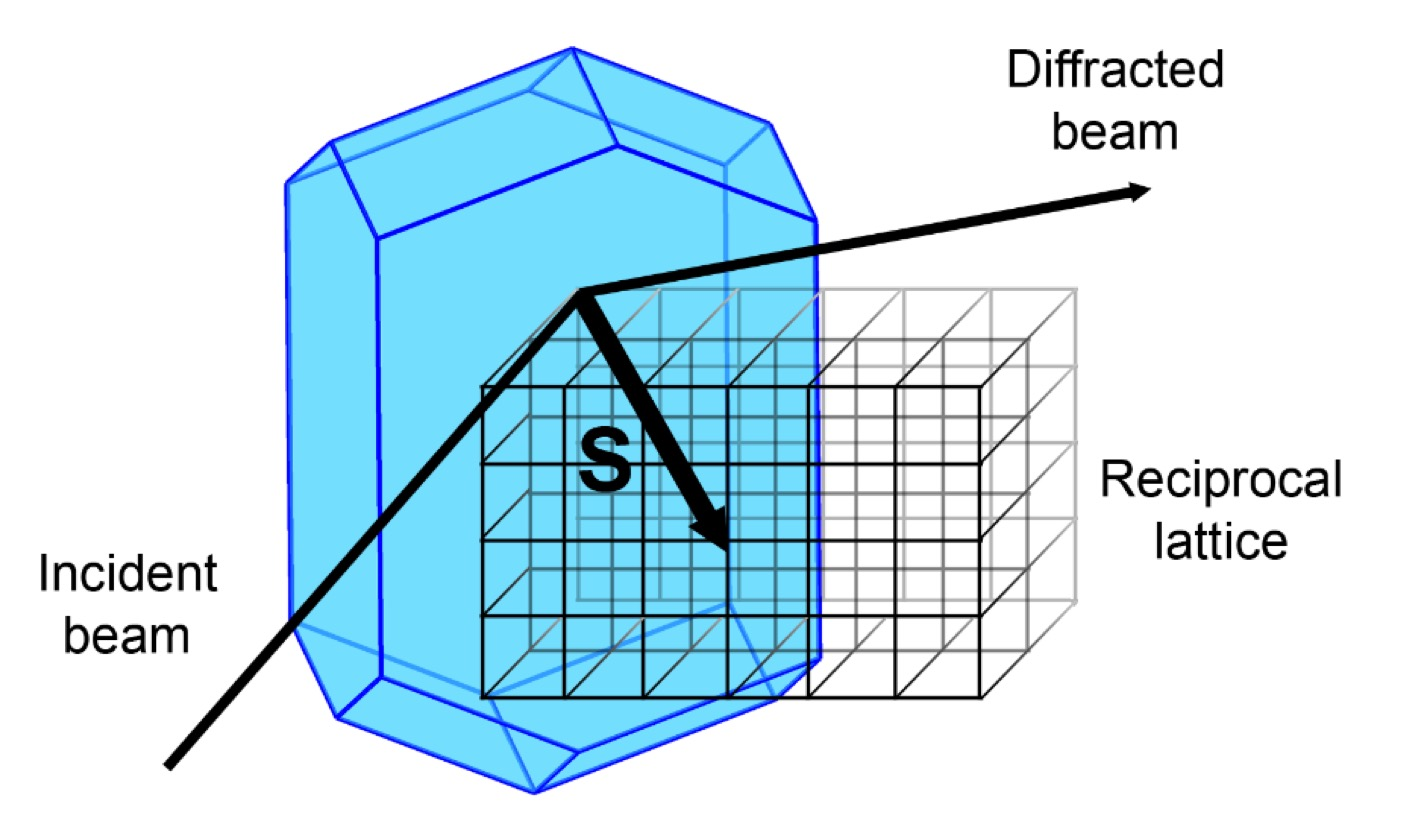
\includegraphics[width=0.6\textwidth]{Single_crystal_diffraction.jpg}
        \caption{A schematic illustration of diffraction in a single crystal.}
    \end{figure}
    
    Practically, it is very difficult to move the X-ray source, so we have to move the crystal and the detector. If the source and the detector are making an angle \(2\theta\), then this will correspond to a scattering vector of length \(2\sin\theta/\lambda\) and direction bisecting the line from the crystal to the source and to the detector. If this scattering vector happens to hit one of the reciprocal lattice point, then we will see a non-zero diffracted intensity in the detector. To make that happen, we have to be able to freely rotate the crystal around all 3 directions, so that we are effectively moving the reciprocal lattice attached to the crystal. This is achieved using a \textit{goniometer}.

    \begin{figure}
        \centering
        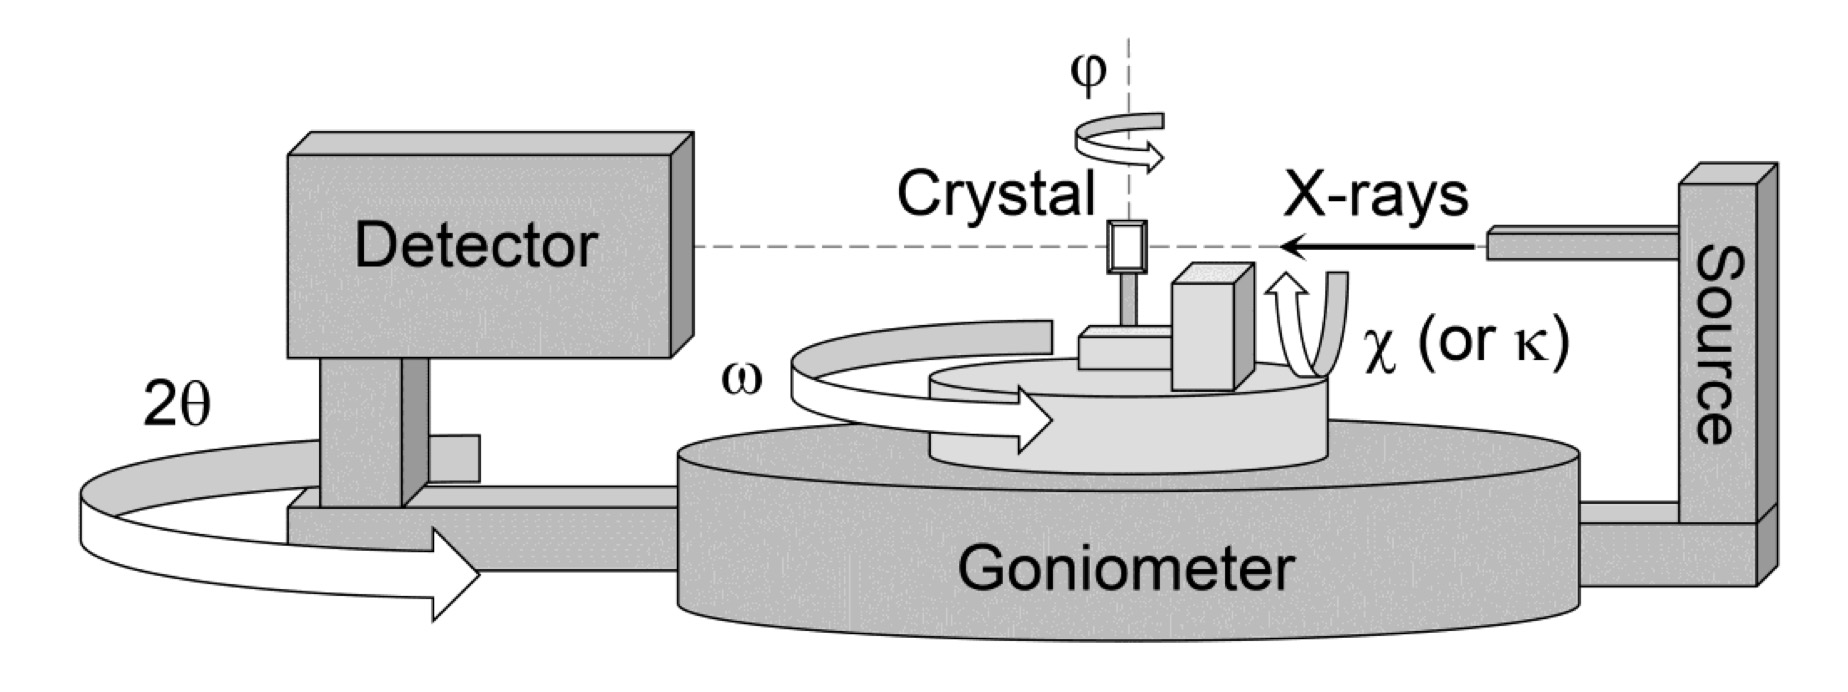
\includegraphics[width=0.7\textwidth]{XRD_apparatus.jpg}
        \caption{Apparatus for measuring the X-ray diffraction of a single crystal practically.}
    \end{figure}

    The outcome of a single-crystal X-ray diffraction measurement can be conceptually divided into two parts.
    \begin{enumerate}[topsep=0pt]
        \item \textit{Geometrical information.} From the value of \(\vb{S}=h\vb{a}^*+k\vb{b}^*+l\vb{c}^*\) we measured non-zero diffraction intensity, we can infer the reciprocal lattice vectors, and hence the real lattice vectors of the crystal. This can be done using only a small proportion of all the diffraction data, so only costs a few minutes.
        \item \textit{A list of diffracted intensity.} Once the geometry of the crystal in known, we can point the crystal and the detector only to where we know that there will be diffraction occurring. Then we can get a list of \(hkl\) values of measured diffracted beams and the corresponding diffraction intensities \(\abs{F(hkl)}^2\). To calculate the Patterson function (or the electron density if we somehow figure out the phases of the beams using methods that will be introduced later), we need the structure factor of the whole reciprocal space. This is not practical to do since there will be some maximum \(\norm{\vb{S}}\) value we are able to reach, and the diffraction will be weak for high \(hkl\) values. What we can do is to measure as many diffracted peaks as possible. This generally take hours, and hence X-ray diffraction is a slow technique, and the resulting structures are usually time-averaged.
    \end{enumerate}

    \subsection{The Independent Atom Model}
    Although \(\rho(\vb{r})\) is a continuous function, we are generally only interested in the positions and types of atoms. We will see how can we make further progress if we introduce an atomic picture.

    We will make the following assumptions.
    \begin{enumerate}[topsep=0pt]
        \item The electron density is not continuous, but instead gathered into isolated, individual atoms at fixed sites. The atoms are spherical.
        \item All electrons are located within atoms. Delocalised electrons or electrons in chemical bonds that are between atoms are neglected.
    \end{enumerate}
    This formalism is known as the \textit{independent atom model} (IAM). The second assumption seems like a fairly suspicious one. As chemists, we all know that chemical structures are held together by chemical bonds, and covalent bonds definitely involve the sharing of atoms. However for most elements, the majority of electrons are core electrons, which are little involved in bonding and are very localised. An obvious exception is hydrogen --- we will discuss more on hydrogen later.

    Now, if we describe the electron density of an atom labelled \(n\) as a spherically symmetric function \(\rho_{\text{atom}, n}(\vb{r})\), then the total electron density in the crystal is
    \begin{equation}
        \rho(\vb{r})=\sum_n \rho_{\text{atom},n}(\vb{r})*\delta(\vb{r}-x_n\vb{a}-y_n\vb{b}-z_n\vb{c})\,,
    \end{equation}
    where \((x_n,y_n,z_n)\) is the fractional coordinate of atom \(n\) and the sum is taken over all atoms in the crystal. Now from the convolution theorem, the structure factor of the cell is
    \begin{align}
        F(\vb{S})&=\mathcal{F}[\rho(\vb{r})]\notag\\
        &=\sum_n\mathcal{F}[\rho_{\text{atom},n}(\vb{r})]\mathcal{F}[\delta(\vb{r}-x_n\vb{a}-y_n\vb{b}-z_n\vb{c})]\notag\\
        &\eqqcolon \sum_n f_n(\vb{S})\exp(2\pi \ii\vb{r}_n\vdot\vb{S})\notag\\
        &=\sum_n f_n(\vb{S})\exp(2\pi \ii(hx_n+ky_n+lz_n))\,,
    \end{align}
    where the \(f_n\) is the Fourier transform of \(\rho_{\text{atom},n}(\vb{r})\) called the \textit{atomic scattering factor}. It can be seen as the diffraction of a single atom, and has unit of electrons. Since we assume \(\rho_{\text{atom},n}(\vb{r})\) is spherically symmetric, \(f(\vb{S})\) is spherically symmetric as well. Although some other more complicated model may apply (e.g. multipole expansion) to make both \(\rho_{\text{atom},n}(\vb{r})\) and \(f(\vb{S})\) not spherically symmetric, we shall not concern with these.

    \subsubsection{Atomic Scattering Factor}
    For the special case of \(\vb{S}=\vb{0}\),
    \begin{equation}
        F(\vb{0})=\sum f_n(\vb{0})=\int\dd{V}\rho(\vb{r})\,.
    \end{equation}
    For this to hold, we must have \(f_n(\vb{0})\) equal to the total number of electrons in atom \(n\). As \(\vb{S}\) moves away from zero, the value of \(f_n\) must change to reflect the interference occurring between X-rays scattered from different positions within the atom's volume. Under the assumption that \(f(\vb{S})\) is spherically symmetric, it is only dependent on \(\norm{\vb{S}}=(2\sin\theta)/\lambda\), so the scattering factor is usually fitted to parameterised function of \((\sin\theta)/\lambda\) as
    \begin{equation}
        f\left(\frac{\sin\theta}{\lambda}\right)=c+\sum_{i=1}^{4}a_i\exp\left[-b_i\left(\frac{\sin\theta}{\lambda}\right)^2\right]
    \end{equation}
    with nine tabulated parameters for each atom. These parameters are known as Cromer--Mann coefficients.

    Some examples of spherically symmetric atomic scattering factors are shown in \cref{Fig:scattering_factor}. We can see that \(f(0)\) is equal to the number of electrons in the atom/ion. Heavier elements generally have larger atomic scattering factors. For species having the same number of electrons, if the atom/ion is larger, than the scattering factors drop off more quickly. This is because a bigger atom would induce a larger path difference in diffraction, and hence leads to lower \(f_n\).\footnote{You can understand this by modelling the electron density in an atom as a Gaussian of width \(\sigma\). Its Fourier transform (the scattering factor) will be a Gaussian of width \(\sigma^{-1}\). Hence, if the atom is larger, then the scattering factor has smaller width. If we have a ``point'' atom, whose electron density is a delta function, then its Fourier transform is a constant, so the scattering factor will not drop off.}
    \begin{figure}
        \centering
        \begin{subfigure}[h]{0.45\linewidth}
            \begin{adjustbox}{width=\linewidth}
                % This file was created with tikzplotlib v0.10.1.
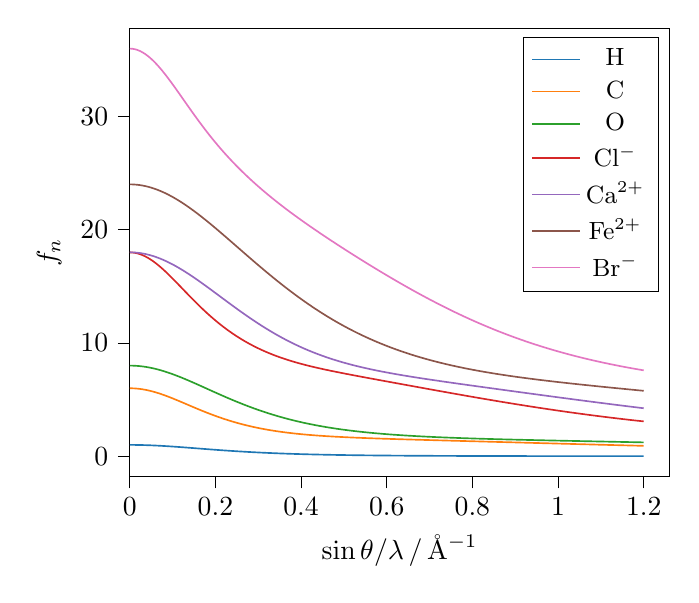
\begin{tikzpicture}

\definecolor{crimson2143940}{RGB}{214,39,40}
\definecolor{darkgray176}{RGB}{176,176,176}
\definecolor{darkorange25512714}{RGB}{255,127,14}
\definecolor{forestgreen4416044}{RGB}{44,160,44}
\definecolor{mediumpurple148103189}{RGB}{148,103,189}
\definecolor{orchid227119194}{RGB}{227,119,194}
\definecolor{sienna1408675}{RGB}{140,86,75}
\definecolor{steelblue31119180}{RGB}{31,119,180}

\begin{axis}[
tick align=outside,
tick pos=left,
x grid style={darkgray176},
xlabel={\(\displaystyle \sin\theta/\lambda \, / \,\)\AA\(\displaystyle ^{-1}\)},
xmin=0, xmax=1.26,
xtick style={color=black},
y grid style={darkgray176},
ylabel={\(\displaystyle f_n\)},
ymin=-1.79405, ymax=37.78505,
ytick style={color=black}
]
\addplot [semithick, steelblue31119180]
table {%
0 1
0.006 0.999
0.0121 0.998
0.0181 0.995
0.0241 0.99
0.0302 0.985
0.0362 0.979
0.0422 0.971
0.0482 0.963
0.0543 0.953
0.0603 0.943
0.0663 0.932
0.0724 0.919
0.0784 0.906
0.0844 0.893
0.0905 0.878
0.0965 0.863
0.1025 0.848
0.1085 0.832
0.1146 0.815
0.1206 0.799
0.1266 0.782
0.1327 0.764
0.1387 0.747
0.1447 0.729
0.1508 0.711
0.1568 0.693
0.1628 0.676
0.1688 0.658
0.1749 0.64
0.1809 0.623
0.1869 0.605
0.193 0.588
0.199 0.571
0.205 0.554
0.2111 0.537
0.2171 0.521
0.2231 0.505
0.2291 0.49
0.2352 0.474
0.2412 0.459
0.2472 0.445
0.2533 0.43
0.2593 0.416
0.2653 0.403
0.2714 0.389
0.2774 0.376
0.2834 0.364
0.2894 0.352
0.2955 0.34
0.3015 0.328
0.3075 0.317
0.3136 0.306
0.3196 0.296
0.3256 0.286
0.3317 0.276
0.3377 0.266
0.3437 0.257
0.3497 0.248
0.3558 0.239
0.3618 0.231
0.3678 0.223
0.3739 0.215
0.3799 0.208
0.3859 0.2
0.392 0.193
0.398 0.187
0.404 0.18
0.4101 0.174
0.4161 0.168
0.4221 0.162
0.4281 0.156
0.4342 0.151
0.4402 0.146
0.4462 0.141
0.4523 0.136
0.4583 0.131
0.4643 0.127
0.4704 0.122
0.4764 0.118
0.4824 0.114
0.4884 0.11
0.4945 0.106
0.5005 0.103
0.5065 0.099
0.5126 0.096
0.5186 0.093
0.5246 0.09
0.5307 0.087
0.5367 0.084
0.5427 0.081
0.5487 0.078
0.5548 0.076
0.5608 0.073
0.5668 0.071
0.5729 0.069
0.5789 0.067
0.5849 0.064
0.591 0.062
0.597 0.06
0.603 0.059
0.609 0.057
0.6151 0.055
0.6211 0.053
0.6271 0.052
0.6332 0.05
0.6392 0.049
0.6452 0.047
0.6513 0.046
0.6573 0.044
0.6633 0.043
0.6693 0.042
0.6754 0.041
0.6814 0.039
0.6874 0.038
0.6935 0.037
0.6995 0.036
0.7055 0.035
0.7116 0.034
0.7176 0.033
0.7236 0.032
0.7296 0.031
0.7357 0.03
0.7417 0.029
0.7477 0.029
0.7538 0.028
0.7598 0.027
0.7658 0.026
0.7719 0.026
0.7779 0.025
0.7839 0.024
0.7899 0.023
0.796 0.023
0.802 0.022
0.808 0.022
0.8141 0.021
0.8201 0.02
0.8261 0.02
0.8322 0.019
0.8382 0.019
0.8442 0.018
0.8503 0.018
0.8563 0.017
0.8623 0.017
0.8683 0.016
0.8744 0.016
0.8804 0.015
0.8864 0.015
0.8925 0.015
0.8985 0.014
0.9045 0.014
0.9106 0.013
0.9166 0.013
0.9226 0.013
0.9286 0.012
0.9347 0.012
0.9407 0.012
0.9467 0.011
0.9528 0.011
0.9588 0.011
0.9648 0.011
0.9709 0.01
0.9769 0.01
0.9829 0.01
0.9889 0.01
0.995 0.009
1.001 0.009
1.007 0.009
1.0131 0.009
1.0191 0.008
1.0251 0.008
1.0312 0.008
1.0372 0.008
1.0432 0.008
1.0492 0.007
1.0553 0.007
1.0613 0.007
1.0673 0.007
1.0734 0.007
1.0794 0.007
1.0854 0.006
1.0915 0.006
1.0975 0.006
1.1035 0.006
1.1095 0.006
1.1156 0.006
1.1216 0.006
1.1276 0.006
1.1337 0.006
1.1397 0.005
1.1457 0.005
1.1518 0.005
1.1578 0.005
1.1638 0.005
1.1698 0.005
1.1759 0.005
1.1819 0.005
1.1879 0.005
1.194 0.005
1.2 0.005
};
\addplot [semithick, darkorange25512714]
table {%
0 5.999
0.006 5.995
0.0121 5.984
0.0181 5.965
0.0241 5.939
0.0302 5.906
0.0362 5.866
0.0422 5.819
0.0482 5.766
0.0543 5.706
0.0603 5.642
0.0663 5.573
0.0724 5.497
0.0784 5.419
0.0844 5.336
0.0905 5.249
0.0965 5.16
0.1025 5.069
0.1085 4.976
0.1146 4.88
0.1206 4.784
0.1266 4.688
0.1327 4.589
0.1387 4.492
0.1447 4.395
0.1508 4.298
0.1568 4.202
0.1628 4.108
0.1688 4.015
0.1749 3.922
0.1809 3.833
0.1869 3.745
0.193 3.657
0.199 3.573
0.205 3.492
0.2111 3.411
0.2171 3.333
0.2231 3.258
0.2291 3.185
0.2352 3.114
0.2412 3.046
0.2472 2.98
0.2533 2.915
0.2593 2.854
0.2653 2.795
0.2714 2.737
0.2774 2.682
0.2834 2.629
0.2894 2.579
0.2955 2.529
0.3015 2.483
0.3075 2.438
0.3136 2.394
0.3196 2.353
0.3256 2.314
0.3317 2.276
0.3377 2.24
0.3437 2.205
0.3497 2.172
0.3558 2.14
0.3618 2.11
0.3678 2.081
0.3739 2.054
0.3799 2.027
0.3859 2.002
0.392 1.978
0.398 1.955
0.404 1.933
0.4101 1.912
0.4161 1.892
0.4221 1.873
0.4281 1.855
0.4342 1.837
0.4402 1.82
0.4462 1.804
0.4523 1.789
0.4583 1.774
0.4643 1.76
0.4704 1.746
0.4764 1.733
0.4824 1.72
0.4884 1.708
0.4945 1.696
0.5005 1.685
0.5065 1.674
0.5126 1.663
0.5186 1.653
0.5246 1.643
0.5307 1.633
0.5367 1.624
0.5427 1.615
0.5487 1.606
0.5548 1.597
0.5608 1.588
0.5668 1.58
0.5729 1.572
0.5789 1.564
0.5849 1.556
0.591 1.548
0.597 1.541
0.603 1.534
0.609 1.526
0.6151 1.519
0.6211 1.512
0.6271 1.505
0.6332 1.498
0.6392 1.491
0.6452 1.484
0.6513 1.477
0.6573 1.471
0.6633 1.464
0.6693 1.458
0.6754 1.451
0.6814 1.445
0.6874 1.438
0.6935 1.432
0.6995 1.425
0.7055 1.419
0.7116 1.413
0.7176 1.406
0.7236 1.4
0.7296 1.394
0.7357 1.387
0.7417 1.381
0.7477 1.375
0.7538 1.369
0.7598 1.362
0.7658 1.356
0.7719 1.35
0.7779 1.344
0.7839 1.338
0.7899 1.331
0.796 1.325
0.802 1.319
0.808 1.313
0.8141 1.307
0.8201 1.3
0.8261 1.294
0.8322 1.288
0.8382 1.282
0.8442 1.276
0.8503 1.269
0.8563 1.263
0.8623 1.257
0.8683 1.251
0.8744 1.244
0.8804 1.238
0.8864 1.232
0.8925 1.226
0.8985 1.22
0.9045 1.213
0.9106 1.207
0.9166 1.201
0.9226 1.195
0.9286 1.189
0.9347 1.182
0.9407 1.176
0.9467 1.17
0.9528 1.164
0.9588 1.157
0.9648 1.151
0.9709 1.145
0.9769 1.139
0.9829 1.133
0.9889 1.127
0.995 1.12
1.001 1.114
1.007 1.108
1.0131 1.102
1.0191 1.096
1.0251 1.09
1.0312 1.083
1.0372 1.077
1.0432 1.071
1.0492 1.065
1.0553 1.059
1.0613 1.053
1.0673 1.047
1.0734 1.041
1.0794 1.035
1.0854 1.029
1.0915 1.022
1.0975 1.016
1.1035 1.01
1.1095 1.004
1.1156 0.998
1.1216 0.992
1.1276 0.986
1.1337 0.98
1.1397 0.975
1.1457 0.969
1.1518 0.963
1.1578 0.957
1.1638 0.951
1.1698 0.945
1.1759 0.939
1.1819 0.933
1.1879 0.928
1.194 0.922
1.2 0.916
};
\addplot [semithick, forestgreen4416044]
table {%
0 7.999
0.006 7.996
0.0121 7.987
0.0181 7.972
0.0241 7.952
0.0302 7.925
0.0362 7.893
0.0422 7.855
0.0482 7.812
0.0543 7.763
0.0603 7.709
0.0663 7.651
0.0724 7.587
0.0784 7.52
0.0844 7.449
0.0905 7.372
0.0965 7.293
0.1025 7.211
0.1085 7.125
0.1146 7.036
0.1206 6.945
0.1266 6.852
0.1327 6.755
0.1387 6.658
0.1447 6.56
0.1508 6.459
0.1568 6.358
0.1628 6.257
0.1688 6.155
0.1749 6.05
0.1809 5.948
0.1869 5.845
0.193 5.741
0.199 5.639
0.205 5.538
0.2111 5.436
0.2171 5.336
0.2231 5.237
0.2291 5.139
0.2352 5.041
0.2412 4.945
0.2472 4.851
0.2533 4.757
0.2593 4.666
0.2653 4.576
0.2714 4.487
0.2774 4.4
0.2834 4.315
0.2894 4.232
0.2955 4.149
0.3015 4.07
0.3075 3.992
0.3136 3.914
0.3196 3.84
0.3256 3.767
0.3317 3.695
0.3377 3.626
0.3437 3.558
0.3497 3.492
0.3558 3.427
0.3618 3.365
0.3678 3.304
0.3739 3.244
0.3799 3.187
0.3859 3.131
0.392 3.076
0.398 3.024
0.404 2.972
0.4101 2.922
0.4161 2.874
0.4221 2.827
0.4281 2.782
0.4342 2.737
0.4402 2.695
0.4462 2.654
0.4523 2.613
0.4583 2.574
0.4643 2.537
0.4704 2.5
0.4764 2.465
0.4824 2.431
0.4884 2.398
0.4945 2.365
0.5005 2.335
0.5065 2.305
0.5126 2.275
0.5186 2.248
0.5246 2.221
0.5307 2.194
0.5367 2.169
0.5427 2.144
0.5487 2.12
0.5548 2.097
0.5608 2.075
0.5668 2.053
0.5729 2.032
0.5789 2.012
0.5849 1.993
0.591 1.973
0.597 1.955
0.603 1.937
0.609 1.92
0.6151 1.903
0.6211 1.887
0.6271 1.872
0.6332 1.856
0.6392 1.842
0.6452 1.827
0.6513 1.813
0.6573 1.8
0.6633 1.787
0.6693 1.774
0.6754 1.762
0.6814 1.75
0.6874 1.738
0.6935 1.727
0.6995 1.716
0.7055 1.705
0.7116 1.694
0.7176 1.684
0.7236 1.674
0.7296 1.665
0.7357 1.655
0.7417 1.646
0.7477 1.637
0.7538 1.628
0.7598 1.62
0.7658 1.612
0.7719 1.603
0.7779 1.595
0.7839 1.588
0.7899 1.58
0.796 1.573
0.802 1.565
0.808 1.558
0.8141 1.551
0.8201 1.544
0.8261 1.538
0.8322 1.531
0.8382 1.524
0.8442 1.518
0.8503 1.512
0.8563 1.505
0.8623 1.499
0.8683 1.493
0.8744 1.487
0.8804 1.481
0.8864 1.476
0.8925 1.47
0.8985 1.464
0.9045 1.459
0.9106 1.453
0.9166 1.448
0.9226 1.442
0.9286 1.437
0.9347 1.432
0.9407 1.427
0.9467 1.421
0.9528 1.416
0.9588 1.411
0.9648 1.406
0.9709 1.401
0.9769 1.396
0.9829 1.391
0.9889 1.386
0.995 1.381
1.001 1.376
1.007 1.371
1.0131 1.366
1.0191 1.362
1.0251 1.357
1.0312 1.352
1.0372 1.347
1.0432 1.342
1.0492 1.338
1.0553 1.333
1.0613 1.328
1.0673 1.323
1.0734 1.319
1.0794 1.314
1.0854 1.309
1.0915 1.305
1.0975 1.3
1.1035 1.295
1.1095 1.291
1.1156 1.286
1.1216 1.281
1.1276 1.277
1.1337 1.272
1.1397 1.267
1.1457 1.263
1.1518 1.258
1.1578 1.254
1.1638 1.249
1.1698 1.244
1.1759 1.24
1.1819 1.235
1.1879 1.231
1.194 1.226
1.2 1.221
};
\addplot [semithick, crimson2143940]
table {%
0 17.994
0.006 17.984
0.0121 17.954
0.0181 17.904
0.0241 17.835
0.0302 17.746
0.0362 17.64
0.0422 17.517
0.0482 17.378
0.0543 17.221
0.0603 17.054
0.0663 16.873
0.0724 16.678
0.0784 16.476
0.0844 16.266
0.0905 16.045
0.0965 15.821
0.1025 15.593
0.1085 15.361
0.1146 15.122
0.1206 14.886
0.1266 14.65
0.1327 14.411
0.1387 14.176
0.1447 13.944
0.1508 13.711
0.1568 13.484
0.1628 13.262
0.1688 13.043
0.1749 12.826
0.1809 12.617
0.1869 12.413
0.193 12.211
0.199 12.017
0.205 11.829
0.2111 11.643
0.2171 11.465
0.2231 11.293
0.2291 11.126
0.2352 10.962
0.2412 10.805
0.2472 10.654
0.2533 10.505
0.2593 10.364
0.2653 10.227
0.2714 10.093
0.2774 9.966
0.2834 9.843
0.2894 9.724
0.2955 9.608
0.3015 9.498
0.3075 9.392
0.3136 9.288
0.3196 9.189
0.3256 9.094
0.3317 9.001
0.3377 8.912
0.3437 8.827
0.3497 8.745
0.3558 8.665
0.3618 8.588
0.3678 8.514
0.3739 8.442
0.3799 8.373
0.3859 8.306
0.392 8.24
0.398 8.178
0.404 8.117
0.4101 8.057
0.4161 7.999
0.4221 7.943
0.4281 7.889
0.4342 7.835
0.4402 7.782
0.4462 7.732
0.4523 7.681
0.4583 7.632
0.4643 7.584
0.4704 7.535
0.4764 7.489
0.4824 7.443
0.4884 7.397
0.4945 7.352
0.5005 7.307
0.5065 7.263
0.5126 7.219
0.5186 7.175
0.5246 7.132
0.5307 7.088
0.5367 7.046
0.5427 7.003
0.5487 6.961
0.5548 6.918
0.5608 6.876
0.5668 6.834
0.5729 6.792
0.5789 6.75
0.5849 6.708
0.591 6.666
0.597 6.624
0.603 6.583
0.609 6.541
0.6151 6.499
0.6211 6.458
0.6271 6.416
0.6332 6.374
0.6392 6.333
0.6452 6.291
0.6513 6.249
0.6573 6.208
0.6633 6.166
0.6693 6.125
0.6754 6.083
0.6814 6.042
0.6874 6.001
0.6935 5.959
0.6995 5.918
0.7055 5.877
0.7116 5.835
0.7176 5.794
0.7236 5.754
0.7296 5.713
0.7357 5.672
0.7417 5.631
0.7477 5.59
0.7538 5.549
0.7598 5.509
0.7658 5.469
0.7719 5.428
0.7779 5.388
0.7839 5.348
0.7899 5.308
0.796 5.268
0.802 5.229
0.808 5.189
0.8141 5.149
0.8201 5.11
0.8261 5.071
0.8322 5.032
0.8382 4.994
0.8442 4.955
0.8503 4.916
0.8563 4.878
0.8623 4.84
0.8683 4.802
0.8744 4.764
0.8804 4.727
0.8864 4.69
0.8925 4.652
0.8985 4.615
0.9045 4.579
0.9106 4.542
0.9166 4.506
0.9226 4.47
0.9286 4.434
0.9347 4.398
0.9407 4.363
0.9467 4.328
0.9528 4.292
0.9588 4.258
0.9648 4.223
0.9709 4.189
0.9769 4.155
0.9829 4.121
0.9889 4.088
0.995 4.054
1.001 4.021
1.007 3.988
1.0131 3.956
1.0191 3.923
1.0251 3.891
1.0312 3.859
1.0372 3.828
1.0432 3.797
1.0492 3.766
1.0553 3.735
1.0613 3.704
1.0673 3.674
1.0734 3.644
1.0794 3.614
1.0854 3.585
1.0915 3.555
1.0975 3.526
1.1035 3.498
1.1095 3.469
1.1156 3.441
1.1216 3.413
1.1276 3.386
1.1337 3.358
1.1397 3.331
1.1457 3.304
1.1518 3.277
1.1578 3.251
1.1638 3.225
1.1698 3.199
1.1759 3.174
1.1819 3.148
1.1879 3.124
1.194 3.099
1.2 3.074
};
\addplot [semithick, mediumpurple148103189]
table {%
0 18.002
0.006 17.998
0.0121 17.986
0.0181 17.965
0.0241 17.937
0.0302 17.899
0.0362 17.854
0.0422 17.802
0.0482 17.742
0.0543 17.673
0.0603 17.598
0.0663 17.516
0.0724 17.425
0.0784 17.329
0.0844 17.227
0.0905 17.117
0.0965 17.003
0.1025 16.883
0.1085 16.758
0.1146 16.625
0.1206 16.49
0.1266 16.351
0.1327 16.205
0.1387 16.058
0.1447 15.907
0.1508 15.751
0.1568 15.595
0.1628 15.436
0.1688 15.274
0.1749 15.109
0.1809 14.944
0.1869 14.778
0.193 14.608
0.199 14.44
0.205 14.272
0.2111 14.101
0.2171 13.932
0.2231 13.764
0.2291 13.597
0.2352 13.427
0.2412 13.261
0.2472 13.096
0.2533 12.929
0.2593 12.767
0.2653 12.606
0.2714 12.445
0.2774 12.288
0.2834 12.133
0.2894 11.98
0.2955 11.827
0.3015 11.679
0.3075 11.533
0.3136 11.387
0.3196 11.247
0.3256 11.109
0.3317 10.971
0.3377 10.839
0.3437 10.709
0.3497 10.582
0.3558 10.455
0.3618 10.334
0.3678 10.215
0.3739 10.097
0.3799 9.984
0.3859 9.874
0.392 9.765
0.398 9.66
0.404 9.558
0.4101 9.457
0.4161 9.361
0.4221 9.267
0.4281 9.175
0.4342 9.085
0.4402 8.999
0.4462 8.915
0.4523 8.832
0.4583 8.752
0.4643 8.675
0.4704 8.599
0.4764 8.526
0.4824 8.456
0.4884 8.387
0.4945 8.319
0.5005 8.254
0.5065 8.191
0.5126 8.129
0.5186 8.069
0.5246 8.011
0.5307 7.954
0.5367 7.899
0.5427 7.845
0.5487 7.793
0.5548 7.742
0.5608 7.692
0.5668 7.643
0.5729 7.595
0.5789 7.549
0.5849 7.504
0.591 7.459
0.597 7.416
0.603 7.373
0.609 7.331
0.6151 7.29
0.6211 7.25
0.6271 7.21
0.6332 7.171
0.6392 7.132
0.6452 7.095
0.6513 7.057
0.6573 7.02
0.6633 6.984
0.6693 6.948
0.6754 6.912
0.6814 6.877
0.6874 6.843
0.6935 6.808
0.6995 6.774
0.7055 6.74
0.7116 6.706
0.7176 6.673
0.7236 6.64
0.7296 6.607
0.7357 6.574
0.7417 6.541
0.7477 6.509
0.7538 6.476
0.7598 6.444
0.7658 6.412
0.7719 6.379
0.7779 6.347
0.7839 6.316
0.7899 6.284
0.796 6.252
0.802 6.22
0.808 6.189
0.8141 6.157
0.8201 6.126
0.8261 6.094
0.8322 6.063
0.8382 6.031
0.8442 6
0.8503 5.969
0.8563 5.937
0.8623 5.906
0.8683 5.875
0.8744 5.844
0.8804 5.813
0.8864 5.782
0.8925 5.75
0.8985 5.719
0.9045 5.688
0.9106 5.657
0.9166 5.626
0.9226 5.595
0.9286 5.565
0.9347 5.533
0.9407 5.503
0.9467 5.472
0.9528 5.441
0.9588 5.41
0.9648 5.38
0.9709 5.349
0.9769 5.318
0.9829 5.288
0.9889 5.258
0.995 5.227
1.001 5.197
1.007 5.166
1.0131 5.136
1.0191 5.106
1.0251 5.076
1.0312 5.045
1.0372 5.015
1.0432 4.985
1.0492 4.956
1.0553 4.925
1.0613 4.896
1.0673 4.866
1.0734 4.836
1.0794 4.807
1.0854 4.778
1.0915 4.748
1.0975 4.719
1.1035 4.69
1.1095 4.661
1.1156 4.631
1.1216 4.603
1.1276 4.574
1.1337 4.545
1.1397 4.516
1.1457 4.488
1.1518 4.459
1.1578 4.431
1.1638 4.403
1.1698 4.375
1.1759 4.347
1.1819 4.319
1.1879 4.291
1.194 4.263
1.2 4.236
};
\addplot [semithick, sienna1408675]
table {%
0 24.001
0.006 23.996
0.0121 23.983
0.0181 23.962
0.0241 23.933
0.0302 23.894
0.0362 23.848
0.0422 23.794
0.0482 23.732
0.0543 23.66
0.0603 23.583
0.0663 23.497
0.0724 23.403
0.0784 23.303
0.0844 23.196
0.0905 23.081
0.0965 22.961
0.1025 22.835
0.1085 22.703
0.1146 22.563
0.1206 22.42
0.1266 22.271
0.1327 22.115
0.1387 21.957
0.1447 21.795
0.1508 21.625
0.1568 21.455
0.1628 21.281
0.1688 21.104
0.1749 20.921
0.1809 20.738
0.1869 20.552
0.193 20.361
0.199 20.172
0.205 19.98
0.2111 19.784
0.2171 19.589
0.2231 19.394
0.2291 19.197
0.2352 18.997
0.2412 18.799
0.2472 18.601
0.2533 18.4
0.2593 18.201
0.2653 18.004
0.2714 17.803
0.2774 17.606
0.2834 17.41
0.2894 17.214
0.2955 17.016
0.3015 16.823
0.3075 16.631
0.3136 16.436
0.3196 16.247
0.3256 16.059
0.3317 15.869
0.3377 15.684
0.3437 15.501
0.3497 15.32
0.3558 15.138
0.3618 14.96
0.3678 14.785
0.3739 14.609
0.3799 14.438
0.3859 14.269
0.392 14.099
0.398 13.935
0.404 13.772
0.4101 13.61
0.4161 13.452
0.4221 13.297
0.4281 13.144
0.4342 12.991
0.4402 12.843
0.4462 12.697
0.4523 12.551
0.4583 12.41
0.4643 12.271
0.4704 12.133
0.4764 11.999
0.4824 11.867
0.4884 11.738
0.4945 11.609
0.5005 11.484
0.5065 11.362
0.5126 11.24
0.5186 11.123
0.5246 11.007
0.5307 10.892
0.5367 10.781
0.5427 10.672
0.5487 10.566
0.5548 10.46
0.5608 10.357
0.5668 10.257
0.5729 10.157
0.5789 10.061
0.5849 9.966
0.591 9.873
0.597 9.782
0.603 9.694
0.609 9.607
0.6151 9.521
0.6211 9.438
0.6271 9.357
0.6332 9.276
0.6392 9.198
0.6452 9.122
0.6513 9.046
0.6573 8.974
0.6633 8.902
0.6693 8.833
0.6754 8.764
0.6814 8.697
0.6874 8.632
0.6935 8.567
0.6995 8.505
0.7055 8.444
0.7116 8.383
0.7176 8.325
0.7236 8.267
0.7296 8.212
0.7357 8.156
0.7417 8.103
0.7477 8.05
0.7538 7.998
0.7598 7.948
0.7658 7.899
0.7719 7.85
0.7779 7.803
0.7839 7.757
0.7899 7.712
0.796 7.667
0.802 7.624
0.808 7.582
0.8141 7.54
0.8201 7.499
0.8261 7.459
0.8322 7.419
0.8382 7.381
0.8442 7.343
0.8503 7.306
0.8563 7.269
0.8623 7.234
0.8683 7.199
0.8744 7.164
0.8804 7.13
0.8864 7.096
0.8925 7.063
0.8985 7.031
0.9045 6.999
0.9106 6.968
0.9166 6.937
0.9226 6.907
0.9286 6.877
0.9347 6.847
0.9407 6.818
0.9467 6.789
0.9528 6.76
0.9588 6.732
0.9648 6.705
0.9709 6.677
0.9769 6.65
0.9829 6.623
0.9889 6.597
0.995 6.57
1.001 6.545
1.007 6.519
1.0131 6.493
1.0191 6.468
1.0251 6.443
1.0312 6.418
1.0372 6.393
1.0432 6.369
1.0492 6.345
1.0553 6.32
1.0613 6.296
1.0673 6.273
1.0734 6.249
1.0794 6.225
1.0854 6.202
1.0915 6.178
1.0975 6.155
1.1035 6.132
1.1095 6.11
1.1156 6.086
1.1216 6.064
1.1276 6.041
1.1337 6.018
1.1397 5.996
1.1457 5.974
1.1518 5.951
1.1578 5.929
1.1638 5.907
1.1698 5.884
1.1759 5.862
1.1819 5.84
1.1879 5.818
1.194 5.796
1.2 5.774
};
\addplot [semithick, orchid227119194]
table {%
0 35.986
0.006 35.972
0.0121 35.931
0.0181 35.863
0.0241 35.768
0.0302 35.647
0.0362 35.502
0.0422 35.335
0.0482 35.145
0.0543 34.931
0.0603 34.702
0.0663 34.456
0.0724 34.19
0.0784 33.915
0.0844 33.628
0.0905 33.325
0.0965 33.02
0.1025 32.707
0.1085 32.39
0.1146 32.064
0.1206 31.74
0.1266 31.416
0.1327 31.087
0.1387 30.765
0.1447 30.445
0.1508 30.122
0.1568 29.809
0.1628 29.5
0.1688 29.195
0.1749 28.891
0.1809 28.597
0.1869 28.308
0.193 28.021
0.199 27.743
0.205 27.472
0.2111 27.201
0.2171 26.941
0.2231 26.686
0.2291 26.436
0.2352 26.187
0.2412 25.947
0.2472 25.712
0.2533 25.478
0.2593 25.252
0.2653 25.03
0.2714 24.809
0.2774 24.595
0.2834 24.385
0.2894 24.179
0.2955 23.972
0.3015 23.772
0.3075 23.576
0.3136 23.379
0.3196 23.188
0.3256 23
0.3317 22.812
0.3377 22.629
0.3437 22.449
0.3497 22.271
0.3558 22.092
0.3618 21.918
0.3678 21.747
0.3739 21.574
0.3799 21.406
0.3859 21.24
0.392 21.072
0.398 20.909
0.404 20.748
0.4101 20.585
0.4161 20.426
0.4221 20.268
0.4281 20.112
0.4342 19.954
0.4402 19.8
0.4462 19.646
0.4523 19.492
0.4583 19.34
0.4643 19.19
0.4704 19.037
0.4764 18.889
0.4824 18.74
0.4884 18.593
0.4945 18.444
0.5005 18.298
0.5065 18.152
0.5126 18.005
0.5186 17.861
0.5246 17.718
0.5307 17.573
0.5367 17.431
0.5427 17.29
0.5487 17.149
0.5548 17.006
0.5608 16.867
0.5668 16.728
0.5729 16.588
0.5789 16.45
0.5849 16.314
0.591 16.175
0.597 16.04
0.603 15.906
0.609 15.772
0.6151 15.637
0.6211 15.505
0.6271 15.373
0.6332 15.241
0.6392 15.111
0.6452 14.982
0.6513 14.852
0.6573 14.725
0.6633 14.599
0.6693 14.474
0.6754 14.347
0.6814 14.224
0.6874 14.102
0.6935 13.978
0.6995 13.858
0.7055 13.739
0.7116 13.619
0.7176 13.501
0.7236 13.385
0.7296 13.27
0.7357 13.154
0.7417 13.041
0.7477 12.929
0.7538 12.817
0.7598 12.707
0.7658 12.599
0.7719 12.49
0.7779 12.383
0.7839 12.278
0.7899 12.174
0.796 12.07
0.802 11.968
0.808 11.868
0.8141 11.767
0.8201 11.669
0.8261 11.572
0.8322 11.475
0.8382 11.38
0.8442 11.286
0.8503 11.193
0.8563 11.101
0.8623 11.011
0.8683 10.923
0.8744 10.834
0.8804 10.747
0.8864 10.662
0.8925 10.576
0.8985 10.493
0.9045 10.411
0.9106 10.329
0.9166 10.249
0.9226 10.171
0.9286 10.093
0.9347 10.016
0.9407 9.94
0.9467 9.866
0.9528 9.792
0.9588 9.72
0.9648 9.649
0.9709 9.578
0.9769 9.509
0.9829 9.441
0.9889 9.374
0.995 9.307
1.001 9.242
1.007 9.179
1.0131 9.115
1.0191 9.053
1.0251 8.992
1.0312 8.931
1.0372 8.872
1.0432 8.814
1.0492 8.757
1.0553 8.699
1.0613 8.644
1.0673 8.589
1.0734 8.535
1.0794 8.482
1.0854 8.43
1.0915 8.378
1.0975 8.328
1.1035 8.278
1.1095 8.229
1.1156 8.181
1.1216 8.134
1.1276 8.087
1.1337 8.041
1.1397 7.996
1.1457 7.951
1.1518 7.907
1.1578 7.864
1.1638 7.822
1.1698 7.781
1.1759 7.739
1.1819 7.699
1.1879 7.66
1.194 7.62
1.2 7.582
};
\addlegendentry{\small\(\mathrm{H}\)}
\addlegendentry{\small\(\mathrm{C}\)}
\addlegendentry{\small\(\mathrm{O}\)}
\addlegendentry{\small\(\mathrm{Cl^-}\)}
\addlegendentry{\small\(\mathrm{Ca^{2+}}\)}
\addlegendentry{\small\(\mathrm{Fe^{2+}}\)}
\addlegendentry{\small\(\mathrm{Br^-}\)}
\end{axis}

\end{tikzpicture}

            \end{adjustbox}
            \caption{Scattering factors of different species with different numbers of electrons.}
        \end{subfigure}
        \hfill
        \begin{subfigure}[h]{0.45\linewidth}
            \begin{adjustbox}{width=\linewidth}
                % This file was created with tikzplotlib v0.10.1.
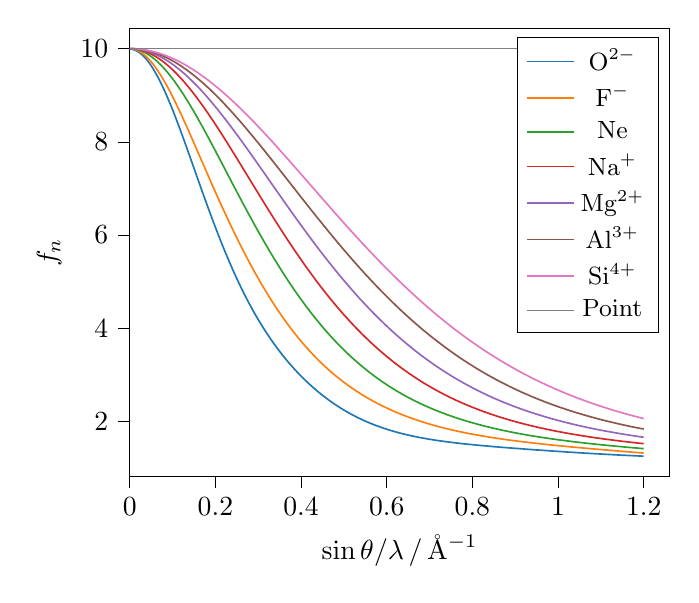
\begin{tikzpicture}

\definecolor{crimson2143940}{RGB}{214,39,40}
\definecolor{darkgray176}{RGB}{176,176,176}
\definecolor{darkorange25512714}{RGB}{255,127,14}
\definecolor{forestgreen4416044}{RGB}{44,160,44}
\definecolor{gray127}{RGB}{127,127,127}
\definecolor{mediumpurple148103189}{RGB}{148,103,189}
\definecolor{orchid227119194}{RGB}{227,119,194}
\definecolor{sienna1408675}{RGB}{140,86,75}
\definecolor{steelblue31119180}{RGB}{31,119,180}

\begin{axis}[
tick align=outside,
tick pos=left,
x grid style={darkgray176},
xlabel={\(\displaystyle \sin\theta/\lambda \, / \,\)\AA\(\displaystyle ^{-1}\)},
xmin=0, xmax=1.26,
xtick style={color=black},
y grid style={darkgray176},
ylabel={\(\displaystyle f_n\)},
ymin=0.8188, ymax=10.4372,
ytick style={color=black}
]
\addplot [semithick, steelblue31119180]
table {%
0 9.989
0.006 9.984
0.0121 9.968
0.0181 9.941
0.0241 9.904
0.0302 9.857
0.0362 9.8
0.0422 9.734
0.0482 9.658
0.0543 9.572
0.0603 9.479
0.0663 9.378
0.0724 9.268
0.0784 9.152
0.0844 9.03
0.0905 8.9
0.0965 8.767
0.1025 8.629
0.1085 8.486
0.1146 8.338
0.1206 8.189
0.1266 8.038
0.1327 7.882
0.1387 7.727
0.1447 7.571
0.1508 7.412
0.1568 7.256
0.1628 7.1
0.1688 6.945
0.1749 6.789
0.1809 6.636
0.1869 6.486
0.193 6.335
0.199 6.189
0.205 6.046
0.2111 5.903
0.2171 5.765
0.2231 5.63
0.2291 5.499
0.2352 5.368
0.2412 5.243
0.2472 5.121
0.2533 5
0.2593 4.885
0.2653 4.773
0.2714 4.662
0.2774 4.556
0.2834 4.454
0.2894 4.354
0.2955 4.256
0.3015 4.163
0.3075 4.072
0.3136 3.983
0.3196 3.897
0.3256 3.815
0.3317 3.733
0.3377 3.655
0.3437 3.58
0.3497 3.507
0.3558 3.435
0.3618 3.366
0.3678 3.299
0.3739 3.234
0.3799 3.171
0.3859 3.11
0.392 3.05
0.398 2.992
0.404 2.937
0.4101 2.882
0.4161 2.83
0.4221 2.779
0.4281 2.73
0.4342 2.681
0.4402 2.635
0.4462 2.59
0.4523 2.546
0.4583 2.504
0.4643 2.463
0.4704 2.423
0.4764 2.384
0.4824 2.347
0.4884 2.312
0.4945 2.276
0.5005 2.243
0.5065 2.211
0.5126 2.179
0.5186 2.149
0.5246 2.12
0.5307 2.091
0.5367 2.064
0.5427 2.038
0.5487 2.013
0.5548 1.989
0.5608 1.966
0.5668 1.943
0.5729 1.921
0.5789 1.901
0.5849 1.881
0.591 1.861
0.597 1.843
0.603 1.825
0.609 1.808
0.6151 1.792
0.6211 1.776
0.6271 1.761
0.6332 1.746
0.6392 1.732
0.6452 1.719
0.6513 1.706
0.6573 1.694
0.6633 1.682
0.6693 1.67
0.6754 1.659
0.6814 1.649
0.6874 1.639
0.6935 1.629
0.6995 1.62
0.7055 1.611
0.7116 1.602
0.7176 1.593
0.7236 1.585
0.7296 1.578
0.7357 1.57
0.7417 1.563
0.7477 1.556
0.7538 1.549
0.7598 1.542
0.7658 1.536
0.7719 1.529
0.7779 1.523
0.7839 1.517
0.7899 1.512
0.796 1.506
0.802 1.501
0.808 1.495
0.8141 1.49
0.8201 1.485
0.8261 1.48
0.8322 1.475
0.8382 1.47
0.8442 1.465
0.8503 1.46
0.8563 1.456
0.8623 1.451
0.8683 1.447
0.8744 1.442
0.8804 1.438
0.8864 1.434
0.8925 1.429
0.8985 1.425
0.9045 1.421
0.9106 1.417
0.9166 1.413
0.9226 1.408
0.9286 1.404
0.9347 1.4
0.9407 1.396
0.9467 1.392
0.9528 1.388
0.9588 1.385
0.9648 1.381
0.9709 1.377
0.9769 1.373
0.9829 1.369
0.9889 1.365
0.995 1.362
1.001 1.358
1.007 1.354
1.0131 1.351
1.0191 1.347
1.0251 1.343
1.0312 1.34
1.0372 1.336
1.0432 1.333
1.0492 1.329
1.0553 1.326
1.0613 1.322
1.0673 1.319
1.0734 1.316
1.0794 1.312
1.0854 1.309
1.0915 1.306
1.0975 1.303
1.1035 1.3
1.1095 1.297
1.1156 1.294
1.1216 1.291
1.1276 1.288
1.1337 1.285
1.1397 1.282
1.1457 1.279
1.1518 1.276
1.1578 1.274
1.1638 1.271
1.1698 1.268
1.1759 1.266
1.1819 1.263
1.1879 1.261
1.194 1.258
1.2 1.256
};
\addplot [semithick, darkorange25512714]
table {%
0 9.998
0.006 9.993
0.0121 9.981
0.0181 9.96
0.0241 9.931
0.0302 9.893
0.0362 9.848
0.0422 9.796
0.0482 9.736
0.0543 9.668
0.0603 9.595
0.0663 9.515
0.0724 9.428
0.0784 9.337
0.0844 9.24
0.0905 9.138
0.0965 9.033
0.1025 8.924
0.1085 8.811
0.1146 8.694
0.1206 8.576
0.1266 8.455
0.1327 8.331
0.1387 8.207
0.1447 8.082
0.1508 7.954
0.1568 7.828
0.1628 7.701
0.1688 7.574
0.1749 7.446
0.1809 7.319
0.1869 7.194
0.193 7.066
0.199 6.942
0.205 6.819
0.2111 6.695
0.2171 6.574
0.2231 6.455
0.2291 6.337
0.2352 6.218
0.2412 6.103
0.2472 5.99
0.2533 5.877
0.2593 5.767
0.2653 5.659
0.2714 5.551
0.2774 5.446
0.2834 5.343
0.2894 5.243
0.2955 5.142
0.3015 5.045
0.3075 4.95
0.3136 4.855
0.3196 4.764
0.3256 4.674
0.3317 4.585
0.3377 4.5
0.3437 4.416
0.3497 4.335
0.3558 4.253
0.3618 4.176
0.3678 4.099
0.3739 4.024
0.3799 3.951
0.3859 3.881
0.392 3.811
0.398 3.744
0.404 3.678
0.4101 3.614
0.4161 3.552
0.4221 3.491
0.4281 3.433
0.4342 3.374
0.4402 3.319
0.4462 3.265
0.4523 3.211
0.4583 3.16
0.4643 3.11
0.4704 3.061
0.4764 3.014
0.4824 2.968
0.4884 2.924
0.4945 2.88
0.5005 2.838
0.5065 2.797
0.5126 2.756
0.5186 2.718
0.5246 2.68
0.5307 2.643
0.5367 2.608
0.5427 2.573
0.5487 2.54
0.5548 2.507
0.5608 2.475
0.5668 2.444
0.5729 2.414
0.5789 2.385
0.5849 2.357
0.591 2.329
0.597 2.302
0.603 2.276
0.609 2.251
0.6151 2.226
0.6211 2.202
0.6271 2.179
0.6332 2.156
0.6392 2.135
0.6452 2.113
0.6513 2.092
0.6573 2.072
0.6633 2.053
0.6693 2.034
0.6754 2.015
0.6814 1.997
0.6874 1.98
0.6935 1.962
0.6995 1.946
0.7055 1.93
0.7116 1.914
0.7176 1.899
0.7236 1.884
0.7296 1.87
0.7357 1.856
0.7417 1.842
0.7477 1.829
0.7538 1.816
0.7598 1.803
0.7658 1.791
0.7719 1.779
0.7779 1.768
0.7839 1.756
0.7899 1.745
0.796 1.734
0.802 1.724
0.808 1.714
0.8141 1.704
0.8201 1.694
0.8261 1.685
0.8322 1.676
0.8382 1.667
0.8442 1.658
0.8503 1.649
0.8563 1.641
0.8623 1.633
0.8683 1.625
0.8744 1.617
0.8804 1.609
0.8864 1.601
0.8925 1.594
0.8985 1.587
0.9045 1.58
0.9106 1.573
0.9166 1.566
0.9226 1.559
0.9286 1.553
0.9347 1.546
0.9407 1.54
0.9467 1.534
0.9528 1.527
0.9588 1.521
0.9648 1.515
0.9709 1.509
0.9769 1.504
0.9829 1.498
0.9889 1.492
0.995 1.487
1.001 1.481
1.007 1.476
1.0131 1.47
1.0191 1.465
1.0251 1.46
1.0312 1.454
1.0372 1.449
1.0432 1.444
1.0492 1.439
1.0553 1.434
1.0613 1.429
1.0673 1.424
1.0734 1.419
1.0794 1.414
1.0854 1.409
1.0915 1.404
1.0975 1.4
1.1035 1.395
1.1095 1.39
1.1156 1.386
1.1216 1.381
1.1276 1.376
1.1337 1.372
1.1397 1.367
1.1457 1.362
1.1518 1.358
1.1578 1.353
1.1638 1.349
1.1698 1.344
1.1759 1.34
1.1819 1.335
1.1879 1.331
1.194 1.326
1.2 1.322
};
\addplot [semithick, forestgreen4416044]
table {%
0 9.999
0.006 9.997
0.0121 9.989
0.0181 9.977
0.0241 9.959
0.0302 9.937
0.0362 9.91
0.0422 9.878
0.0482 9.842
0.0543 9.8
0.0603 9.755
0.0663 9.705
0.0724 9.65
0.0784 9.592
0.0844 9.53
0.0905 9.464
0.0965 9.394
0.1025 9.322
0.1085 9.246
0.1146 9.165
0.1206 9.083
0.1266 8.998
0.1327 8.909
0.1387 8.819
0.1447 8.727
0.1508 8.632
0.1568 8.535
0.1628 8.438
0.1688 8.339
0.1749 8.236
0.1809 8.135
0.1869 8.032
0.193 7.926
0.199 7.822
0.205 7.717
0.2111 7.61
0.2171 7.505
0.2231 7.399
0.2291 7.293
0.2352 7.186
0.2412 7.08
0.2472 6.975
0.2533 6.869
0.2593 6.765
0.2653 6.661
0.2714 6.557
0.2774 6.455
0.2834 6.354
0.2894 6.253
0.2955 6.152
0.3015 6.054
0.3075 5.957
0.3136 5.859
0.3196 5.764
0.3256 5.671
0.3317 5.577
0.3377 5.486
0.3437 5.396
0.3497 5.307
0.3558 5.218
0.3618 5.132
0.3678 5.048
0.3739 4.963
0.3799 4.882
0.3859 4.801
0.392 4.721
0.398 4.644
0.404 4.568
0.4101 4.492
0.4161 4.418
0.4221 4.346
0.4281 4.276
0.4342 4.206
0.4402 4.138
0.4462 4.071
0.4523 4.005
0.4583 3.942
0.4643 3.879
0.4704 3.817
0.4764 3.758
0.4824 3.699
0.4884 3.642
0.4945 3.585
0.5005 3.531
0.5065 3.477
0.5126 3.424
0.5186 3.373
0.5246 3.323
0.5307 3.274
0.5367 3.226
0.5427 3.18
0.5487 3.135
0.5548 3.09
0.5608 3.047
0.5668 3.004
0.5729 2.963
0.5789 2.923
0.5849 2.883
0.591 2.845
0.597 2.808
0.603 2.771
0.609 2.736
0.6151 2.701
0.6211 2.667
0.6271 2.634
0.6332 2.602
0.6392 2.571
0.6452 2.54
0.6513 2.51
0.6573 2.481
0.6633 2.453
0.6693 2.426
0.6754 2.399
0.6814 2.373
0.6874 2.347
0.6935 2.322
0.6995 2.298
0.7055 2.274
0.7116 2.251
0.7176 2.229
0.7236 2.207
0.7296 2.186
0.7357 2.165
0.7417 2.144
0.7477 2.125
0.7538 2.105
0.7598 2.086
0.7658 2.068
0.7719 2.05
0.7779 2.033
0.7839 2.016
0.7899 1.999
0.796 1.983
0.802 1.967
0.808 1.952
0.8141 1.936
0.8201 1.922
0.8261 1.907
0.8322 1.893
0.8382 1.88
0.8442 1.866
0.8503 1.853
0.8563 1.841
0.8623 1.828
0.8683 1.816
0.8744 1.804
0.8804 1.793
0.8864 1.781
0.8925 1.77
0.8985 1.759
0.9045 1.749
0.9106 1.738
0.9166 1.728
0.9226 1.718
0.9286 1.709
0.9347 1.699
0.9407 1.69
0.9467 1.681
0.9528 1.672
0.9588 1.663
0.9648 1.655
0.9709 1.647
0.9769 1.638
0.9829 1.63
0.9889 1.623
0.995 1.615
1.001 1.607
1.007 1.6
1.0131 1.593
1.0191 1.586
1.0251 1.579
1.0312 1.572
1.0372 1.565
1.0432 1.558
1.0492 1.552
1.0553 1.546
1.0613 1.539
1.0673 1.533
1.0734 1.527
1.0794 1.521
1.0854 1.515
1.0915 1.509
1.0975 1.504
1.1035 1.498
1.1095 1.493
1.1156 1.487
1.1216 1.482
1.1276 1.476
1.1337 1.471
1.1397 1.466
1.1457 1.461
1.1518 1.456
1.1578 1.451
1.1638 1.446
1.1698 1.441
1.1759 1.436
1.1819 1.432
1.1879 1.427
1.194 1.422
1.2 1.418
};
\addplot [semithick, crimson2143940]
table {%
0 10
0.006 9.998
0.0121 9.993
0.0181 9.984
0.0241 9.972
0.0302 9.957
0.0362 9.938
0.0422 9.916
0.0482 9.891
0.0543 9.862
0.0603 9.831
0.0663 9.796
0.0724 9.758
0.0784 9.717
0.0844 9.673
0.0905 9.626
0.0965 9.576
0.1025 9.524
0.1085 9.47
0.1146 9.411
0.1206 9.351
0.1266 9.289
0.1327 9.224
0.1387 9.157
0.1447 9.088
0.1508 9.016
0.1568 8.944
0.1628 8.869
0.1688 8.793
0.1749 8.714
0.1809 8.635
0.1869 8.554
0.193 8.471
0.199 8.388
0.205 8.304
0.2111 8.217
0.2171 8.131
0.2231 8.044
0.2291 7.956
0.2352 7.866
0.2412 7.777
0.2472 7.688
0.2533 7.597
0.2593 7.507
0.2653 7.416
0.2714 7.324
0.2774 7.234
0.2834 7.144
0.2894 7.053
0.2955 6.962
0.3015 6.872
0.3075 6.782
0.3136 6.691
0.3196 6.602
0.3256 6.514
0.3317 6.424
0.3377 6.337
0.3437 6.25
0.3497 6.164
0.3558 6.077
0.3618 5.992
0.3678 5.908
0.3739 5.823
0.3799 5.741
0.3859 5.659
0.392 5.577
0.398 5.497
0.404 5.418
0.4101 5.339
0.4161 5.262
0.4221 5.186
0.4281 5.111
0.4342 5.035
0.4402 4.962
0.4462 4.89
0.4523 4.818
0.4583 4.748
0.4643 4.679
0.4704 4.61
0.4764 4.543
0.4824 4.478
0.4884 4.413
0.4945 4.348
0.5005 4.285
0.5065 4.224
0.5126 4.162
0.5186 4.103
0.5246 4.044
0.5307 3.986
0.5367 3.93
0.5427 3.874
0.5487 3.82
0.5548 3.766
0.5608 3.713
0.5668 3.662
0.5729 3.611
0.5789 3.561
0.5849 3.513
0.591 3.465
0.597 3.418
0.603 3.372
0.609 3.328
0.6151 3.283
0.6211 3.24
0.6271 3.198
0.6332 3.156
0.6392 3.116
0.6452 3.076
0.6513 3.037
0.6573 2.999
0.6633 2.962
0.6693 2.926
0.6754 2.89
0.6814 2.855
0.6874 2.821
0.6935 2.787
0.6995 2.755
0.7055 2.723
0.7116 2.691
0.7176 2.661
0.7236 2.631
0.7296 2.602
0.7357 2.573
0.7417 2.545
0.7477 2.518
0.7538 2.491
0.7598 2.465
0.7658 2.44
0.7719 2.414
0.7779 2.39
0.7839 2.366
0.7899 2.343
0.796 2.32
0.802 2.298
0.808 2.276
0.8141 2.254
0.8201 2.234
0.8261 2.213
0.8322 2.193
0.8382 2.174
0.8442 2.155
0.8503 2.136
0.8563 2.118
0.8623 2.1
0.8683 2.083
0.8744 2.066
0.8804 2.049
0.8864 2.033
0.8925 2.017
0.8985 2.001
0.9045 1.986
0.9106 1.971
0.9166 1.957
0.9226 1.943
0.9286 1.929
0.9347 1.915
0.9407 1.902
0.9467 1.889
0.9528 1.876
0.9588 1.863
0.9648 1.851
0.9709 1.839
0.9769 1.827
0.9829 1.816
0.9889 1.805
0.995 1.794
1.001 1.783
1.007 1.773
1.0131 1.762
1.0191 1.752
1.0251 1.742
1.0312 1.732
1.0372 1.723
1.0432 1.714
1.0492 1.705
1.0553 1.696
1.0613 1.687
1.0673 1.678
1.0734 1.67
1.0794 1.661
1.0854 1.653
1.0915 1.645
1.0975 1.638
1.1035 1.63
1.1095 1.622
1.1156 1.615
1.1216 1.608
1.1276 1.601
1.1337 1.594
1.1397 1.587
1.1457 1.58
1.1518 1.573
1.1578 1.567
1.1638 1.56
1.1698 1.554
1.1759 1.548
1.1819 1.542
1.1879 1.536
1.194 1.53
1.2 1.524
};
\addplot [semithick, mediumpurple148103189]
table {%
0 10
0.006 9.999
0.0121 9.995
0.0181 9.989
0.0241 9.98
0.0302 9.968
0.0362 9.955
0.0422 9.939
0.0482 9.92
0.0543 9.899
0.0603 9.875
0.0663 9.849
0.0724 9.821
0.0784 9.79
0.0844 9.758
0.0905 9.722
0.0965 9.685
0.1025 9.646
0.1085 9.604
0.1146 9.56
0.1206 9.515
0.1266 9.468
0.1327 9.417
0.1387 9.366
0.1447 9.313
0.1508 9.258
0.1568 9.202
0.1628 9.144
0.1688 9.084
0.1749 9.022
0.1809 8.959
0.1869 8.896
0.193 8.829
0.199 8.763
0.205 8.695
0.2111 8.625
0.2171 8.555
0.2231 8.485
0.2291 8.413
0.2352 8.339
0.2412 8.265
0.2472 8.191
0.2533 8.115
0.2593 8.039
0.2653 7.963
0.2714 7.885
0.2774 7.808
0.2834 7.73
0.2894 7.652
0.2955 7.572
0.3015 7.494
0.3075 7.415
0.3136 7.335
0.3196 7.256
0.3256 7.177
0.3317 7.096
0.3377 7.017
0.3437 6.938
0.3497 6.86
0.3558 6.78
0.3618 6.701
0.3678 6.623
0.3739 6.544
0.3799 6.467
0.3859 6.389
0.392 6.311
0.398 6.235
0.404 6.159
0.4101 6.082
0.4161 6.008
0.4221 5.933
0.4281 5.859
0.4342 5.785
0.4402 5.712
0.4462 5.64
0.4523 5.568
0.4583 5.497
0.4643 5.427
0.4704 5.357
0.4764 5.288
0.4824 5.22
0.4884 5.153
0.4945 5.085
0.5005 5.02
0.5065 4.955
0.5126 4.89
0.5186 4.826
0.5246 4.764
0.5307 4.701
0.5367 4.64
0.5427 4.58
0.5487 4.521
0.5548 4.461
0.5608 4.404
0.5668 4.347
0.5729 4.29
0.5789 4.234
0.5849 4.18
0.591 4.126
0.597 4.073
0.603 4.021
0.609 3.969
0.6151 3.918
0.6211 3.869
0.6271 3.82
0.6332 3.771
0.6392 3.724
0.6452 3.677
0.6513 3.631
0.6573 3.586
0.6633 3.542
0.6693 3.498
0.6754 3.455
0.6814 3.413
0.6874 3.372
0.6935 3.331
0.6995 3.291
0.7055 3.252
0.7116 3.213
0.7176 3.175
0.7236 3.138
0.7296 3.102
0.7357 3.066
0.7417 3.031
0.7477 2.997
0.7538 2.962
0.7598 2.929
0.7658 2.897
0.7719 2.865
0.7779 2.833
0.7839 2.803
0.7899 2.773
0.796 2.743
0.802 2.714
0.808 2.686
0.8141 2.658
0.8201 2.63
0.8261 2.604
0.8322 2.577
0.8382 2.551
0.8442 2.526
0.8503 2.501
0.8563 2.477
0.8623 2.453
0.8683 2.43
0.8744 2.407
0.8804 2.385
0.8864 2.363
0.8925 2.341
0.8985 2.32
0.9045 2.3
0.9106 2.279
0.9166 2.26
0.9226 2.24
0.9286 2.221
0.9347 2.202
0.9407 2.184
0.9467 2.166
0.9528 2.149
0.9588 2.132
0.9648 2.115
0.9709 2.098
0.9769 2.082
0.9829 2.066
0.9889 2.051
0.995 2.035
1.001 2.02
1.007 2.006
1.0131 1.991
1.0191 1.977
1.0251 1.964
1.0312 1.95
1.0372 1.937
1.0432 1.924
1.0492 1.911
1.0553 1.899
1.0613 1.886
1.0673 1.875
1.0734 1.863
1.0794 1.851
1.0854 1.84
1.0915 1.829
1.0975 1.818
1.1035 1.807
1.1095 1.797
1.1156 1.787
1.1216 1.777
1.1276 1.767
1.1337 1.757
1.1397 1.747
1.1457 1.738
1.1518 1.729
1.1578 1.72
1.1638 1.711
1.1698 1.703
1.1759 1.694
1.1819 1.686
1.1879 1.677
1.194 1.669
1.2 1.661
};
\addplot [semithick, sienna1408675]
table {%
0 10
0.006 9.999
0.0121 9.996
0.0181 9.991
0.0241 9.984
0.0302 9.976
0.0362 9.965
0.0422 9.952
0.0482 9.938
0.0543 9.921
0.0603 9.903
0.0663 9.883
0.0724 9.861
0.0784 9.837
0.0844 9.812
0.0905 9.784
0.0965 9.755
0.1025 9.725
0.1085 9.692
0.1146 9.657
0.1206 9.622
0.1266 9.584
0.1327 9.545
0.1387 9.504
0.1447 9.462
0.1508 9.418
0.1568 9.373
0.1628 9.327
0.1688 9.279
0.1749 9.23
0.1809 9.179
0.1869 9.128
0.193 9.074
0.199 9.02
0.205 8.965
0.2111 8.908
0.2171 8.851
0.2231 8.792
0.2291 8.733
0.2352 8.672
0.2412 8.611
0.2472 8.549
0.2533 8.485
0.2593 8.422
0.2653 8.358
0.2714 8.292
0.2774 8.226
0.2834 8.16
0.2894 8.094
0.2955 8.025
0.3015 7.958
0.3075 7.89
0.3136 7.82
0.3196 7.751
0.3256 7.682
0.3317 7.612
0.3377 7.542
0.3437 7.472
0.3497 7.402
0.3558 7.331
0.3618 7.261
0.3678 7.19
0.3739 7.119
0.3799 7.049
0.3859 6.978
0.392 6.907
0.398 6.837
0.404 6.767
0.4101 6.696
0.4161 6.626
0.4221 6.556
0.4281 6.487
0.4342 6.417
0.4402 6.348
0.4462 6.28
0.4523 6.21
0.4583 6.143
0.4643 6.075
0.4704 6.007
0.4764 5.94
0.4824 5.874
0.4884 5.808
0.4945 5.742
0.5005 5.677
0.5065 5.613
0.5126 5.548
0.5186 5.484
0.5246 5.422
0.5307 5.358
0.5367 5.297
0.5427 5.235
0.5487 5.175
0.5548 5.114
0.5608 5.054
0.5668 4.995
0.5729 4.936
0.5789 4.879
0.5849 4.822
0.591 4.764
0.597 4.708
0.603 4.653
0.609 4.599
0.6151 4.544
0.6211 4.491
0.6271 4.438
0.6332 4.385
0.6392 4.334
0.6452 4.283
0.6513 4.233
0.6573 4.183
0.6633 4.134
0.6693 4.086
0.6754 4.038
0.6814 3.991
0.6874 3.945
0.6935 3.899
0.6995 3.854
0.7055 3.81
0.7116 3.766
0.7176 3.723
0.7236 3.681
0.7296 3.639
0.7357 3.597
0.7417 3.557
0.7477 3.517
0.7538 3.477
0.7598 3.438
0.7658 3.4
0.7719 3.362
0.7779 3.325
0.7839 3.289
0.7899 3.253
0.796 3.218
0.802 3.183
0.808 3.149
0.8141 3.115
0.8201 3.082
0.8261 3.05
0.8322 3.018
0.8382 2.986
0.8442 2.956
0.8503 2.925
0.8563 2.895
0.8623 2.866
0.8683 2.837
0.8744 2.809
0.8804 2.781
0.8864 2.753
0.8925 2.726
0.8985 2.7
0.9045 2.674
0.9106 2.648
0.9166 2.623
0.9226 2.599
0.9286 2.575
0.9347 2.551
0.9407 2.527
0.9467 2.504
0.9528 2.482
0.9588 2.46
0.9648 2.438
0.9709 2.416
0.9769 2.395
0.9829 2.375
0.9889 2.355
0.995 2.335
1.001 2.315
1.007 2.296
1.0131 2.277
1.0191 2.259
1.0251 2.241
1.0312 2.223
1.0372 2.205
1.0432 2.188
1.0492 2.172
1.0553 2.155
1.0613 2.139
1.0673 2.123
1.0734 2.107
1.0794 2.092
1.0854 2.077
1.0915 2.062
1.0975 2.047
1.1035 2.033
1.1095 2.019
1.1156 2.005
1.1216 1.992
1.1276 1.979
1.1337 1.966
1.1397 1.953
1.1457 1.94
1.1518 1.928
1.1578 1.916
1.1638 1.904
1.1698 1.892
1.1759 1.881
1.1819 1.87
1.1879 1.859
1.194 1.848
1.2 1.837
};
\addplot [semithick, orchid227119194]
table {%
0 10
0.006 9.999
0.0121 9.997
0.0181 9.993
0.0241 9.988
0.0302 9.981
0.0362 9.972
0.0422 9.962
0.0482 9.951
0.0543 9.937
0.0603 9.923
0.0663 9.907
0.0724 9.889
0.0784 9.87
0.0844 9.85
0.0905 9.828
0.0965 9.804
0.1025 9.78
0.1085 9.754
0.1146 9.726
0.1206 9.697
0.1266 9.667
0.1327 9.635
0.1387 9.602
0.1447 9.568
0.1508 9.532
0.1568 9.496
0.1628 9.458
0.1688 9.419
0.1749 9.378
0.1809 9.337
0.1869 9.295
0.193 9.251
0.199 9.206
0.205 9.161
0.2111 9.114
0.2171 9.066
0.2231 9.018
0.2291 8.968
0.2352 8.917
0.2412 8.866
0.2472 8.815
0.2533 8.761
0.2593 8.708
0.2653 8.653
0.2714 8.598
0.2774 8.542
0.2834 8.486
0.2894 8.429
0.2955 8.371
0.3015 8.313
0.3075 8.254
0.3136 8.194
0.3196 8.135
0.3256 8.075
0.3317 8.013
0.3377 7.953
0.3437 7.892
0.3497 7.83
0.3558 7.767
0.3618 7.705
0.3678 7.643
0.3739 7.58
0.3799 7.517
0.3859 7.454
0.392 7.39
0.398 7.327
0.404 7.264
0.4101 7.2
0.4161 7.136
0.4221 7.073
0.4281 7.01
0.4342 6.945
0.4402 6.882
0.4462 6.819
0.4523 6.755
0.4583 6.692
0.4643 6.629
0.4704 6.565
0.4764 6.503
0.4824 6.44
0.4884 6.378
0.4945 6.315
0.5005 6.253
0.5065 6.192
0.5126 6.13
0.5186 6.069
0.5246 6.008
0.5307 5.947
0.5367 5.887
0.5427 5.827
0.5487 5.768
0.5548 5.708
0.5608 5.65
0.5668 5.592
0.5729 5.533
0.5789 5.476
0.5849 5.419
0.591 5.361
0.597 5.305
0.603 5.25
0.609 5.195
0.6151 5.139
0.6211 5.085
0.6271 5.031
0.6332 4.977
0.6392 4.924
0.6452 4.872
0.6513 4.819
0.6573 4.768
0.6633 4.717
0.6693 4.667
0.6754 4.616
0.6814 4.567
0.6874 4.518
0.6935 4.469
0.6995 4.422
0.7055 4.374
0.7116 4.327
0.7176 4.281
0.7236 4.235
0.7296 4.19
0.7357 4.145
0.7417 4.101
0.7477 4.058
0.7538 4.014
0.7598 3.971
0.7658 3.93
0.7719 3.887
0.7779 3.847
0.7839 3.806
0.7899 3.766
0.796 3.726
0.802 3.688
0.808 3.649
0.8141 3.611
0.8201 3.574
0.8261 3.537
0.8322 3.5
0.8382 3.464
0.8442 3.429
0.8503 3.394
0.8563 3.359
0.8623 3.326
0.8683 3.292
0.8744 3.259
0.8804 3.227
0.8864 3.195
0.8925 3.163
0.8985 3.132
0.9045 3.101
0.9106 3.071
0.9166 3.041
0.9226 3.012
0.9286 2.983
0.9347 2.954
0.9407 2.926
0.9467 2.899
0.9528 2.872
0.9588 2.845
0.9648 2.819
0.9709 2.793
0.9769 2.767
0.9829 2.742
0.9889 2.718
0.995 2.693
1.001 2.669
1.007 2.646
1.0131 2.622
1.0191 2.599
1.0251 2.577
1.0312 2.555
1.0372 2.533
1.0432 2.512
1.0492 2.491
1.0553 2.47
1.0613 2.45
1.0673 2.43
1.0734 2.41
1.0794 2.39
1.0854 2.371
1.0915 2.352
1.0975 2.334
1.1035 2.316
1.1095 2.298
1.1156 2.28
1.1216 2.263
1.1276 2.246
1.1337 2.229
1.1397 2.213
1.1457 2.197
1.1518 2.181
1.1578 2.165
1.1638 2.15
1.1698 2.135
1.1759 2.12
1.1819 2.106
1.1879 2.091
1.194 2.077
1.2 2.063
};
\addplot [semithick, gray127]
table {%
0 10
0.006 10
0.0121 10
0.0181 10
0.0241 10
0.0302 10
0.0362 10
0.0422 10
0.0482 10
0.0543 10
0.0603 10
0.0663 10
0.0724 10
0.0784 10
0.0844 10
0.0905 10
0.0965 10
0.1025 10
0.1085 10
0.1146 10
0.1206 10
0.1266 10
0.1327 10
0.1387 10
0.1447 10
0.1508 10
0.1568 10
0.1628 10
0.1688 10
0.1749 10
0.1809 10
0.1869 10
0.193 10
0.199 10
0.205 10
0.2111 10
0.2171 10
0.2231 10
0.2291 10
0.2352 10
0.2412 10
0.2472 10
0.2533 10
0.2593 10
0.2653 10
0.2714 10
0.2774 10
0.2834 10
0.2894 10
0.2955 10
0.3015 10
0.3075 10
0.3136 10
0.3196 10
0.3256 10
0.3317 10
0.3377 10
0.3437 10
0.3497 10
0.3558 10
0.3618 10
0.3678 10
0.3739 10
0.3799 10
0.3859 10
0.392 10
0.398 10
0.404 10
0.4101 10
0.4161 10
0.4221 10
0.4281 10
0.4342 10
0.4402 10
0.4462 10
0.4523 10
0.4583 10
0.4643 10
0.4704 10
0.4764 10
0.4824 10
0.4884 10
0.4945 10
0.5005 10
0.5065 10
0.5126 10
0.5186 10
0.5246 10
0.5307 10
0.5367 10
0.5427 10
0.5487 10
0.5548 10
0.5608 10
0.5668 10
0.5729 10
0.5789 10
0.5849 10
0.591 10
0.597 10
0.603 10
0.609 10
0.6151 10
0.6211 10
0.6271 10
0.6332 10
0.6392 10
0.6452 10
0.6513 10
0.6573 10
0.6633 10
0.6693 10
0.6754 10
0.6814 10
0.6874 10
0.6935 10
0.6995 10
0.7055 10
0.7116 10
0.7176 10
0.7236 10
0.7296 10
0.7357 10
0.7417 10
0.7477 10
0.7538 10
0.7598 10
0.7658 10
0.7719 10
0.7779 10
0.7839 10
0.7899 10
0.796 10
0.802 10
0.808 10
0.8141 10
0.8201 10
0.8261 10
0.8322 10
0.8382 10
0.8442 10
0.8503 10
0.8563 10
0.8623 10
0.8683 10
0.8744 10
0.8804 10
0.8864 10
0.8925 10
0.8985 10
0.9045 10
0.9106 10
0.9166 10
0.9226 10
0.9286 10
0.9347 10
0.9407 10
0.9467 10
0.9528 10
0.9588 10
0.9648 10
0.9709 10
0.9769 10
0.9829 10
0.9889 10
0.995 10
1.001 10
1.007 10
1.0131 10
1.0191 10
1.0251 10
1.0312 10
1.0372 10
1.0432 10
1.0492 10
1.0553 10
1.0613 10
1.0673 10
1.0734 10
1.0794 10
1.0854 10
1.0915 10
1.0975 10
1.1035 10
1.1095 10
1.1156 10
1.1216 10
1.1276 10
1.1337 10
1.1397 10
1.1457 10
1.1518 10
1.1578 10
1.1638 10
1.1698 10
1.1759 10
1.1819 10
1.1879 10
1.194 10
1.2 10
};
\addlegendentry{\small\(\mathrm{O^{2-}}\)}
\addlegendentry{\small\(\mathrm{F^-}\)}
\addlegendentry{\small\(\mathrm{Ne}\)}
\addlegendentry{\small\(\mathrm{Na^+}\)}
\addlegendentry{\small\(\mathrm{Mg^{2+}}\)}
\addlegendentry{\small\(\mathrm{Al^{3+}}\)}
\addlegendentry{\small\(\mathrm{Si^{4+}}\)}
\addlegendentry{\small Point}
\end{axis}

\end{tikzpicture}

            \end{adjustbox}
            \caption{Scattering factors of different species with the same number of electrons.}
        \end{subfigure}
        \caption{Atomic scattering factors of different species.}
        \label{Fig:scattering_factor}
    \end{figure}

    These factors are derived quantum mechanically from atomic wavefunctions, which are effectively at \(0\unit{K}\). In practice, atoms in crystals are typically slightly displaced from their average position --- this may be dynamic (due to thermal vibration) or static. This effectively makes the atom look larger, and hence the atomic scattering factor will drop off more quickly. This will put an extra \textit{Debye--Waller factor}
    \begin{equation}
        \exp\left(-\frac{8\pi^2\eval{u^2}\sin^2\theta}{\lambda^2}\right)
    \end{equation}
    onto the atomic scattering factor at \(0\unit{K}\).

    \begin{figure}
        \centering
        % This file was created with tikzplotlib v0.10.1.
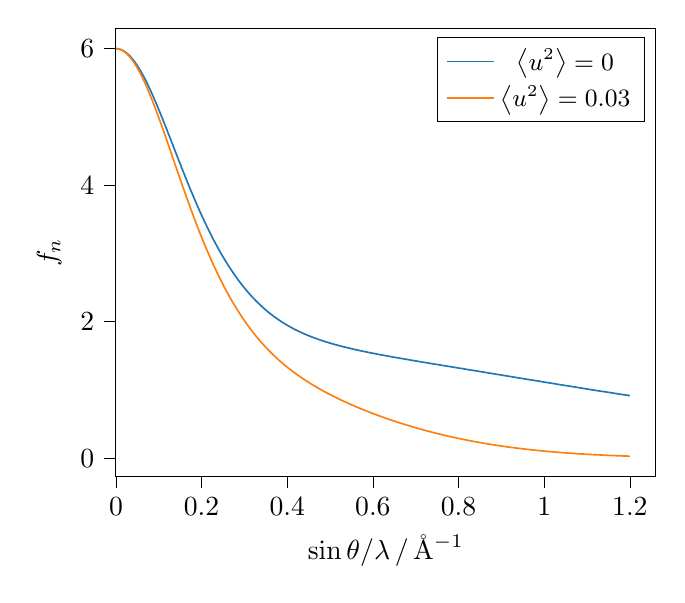
\begin{tikzpicture}

\definecolor{darkgray176}{RGB}{176,176,176}
\definecolor{darkorange25512714}{RGB}{255,127,14}
\definecolor{steelblue31119180}{RGB}{31,119,180}

\begin{axis}[
tick align=outside,
tick pos=left,
x grid style={darkgray176},
xlabel={\(\displaystyle \sin\theta/\lambda \, / \,\)\AA\(\displaystyle ^{-1}\)},
xmin=0, xmax=1.26,
xtick style={color=black},
y grid style={darkgray176},
ylabel={\(\displaystyle f_n\)},
ymin=-0.26845, ymax=6.29745,
ytick style={color=black}
]
\addplot [semithick, steelblue31119180]
table {%
0 5.999
0.006 5.995
0.0121 5.984
0.0181 5.965
0.0241 5.939
0.0302 5.906
0.0362 5.866
0.0422 5.819
0.0482 5.766
0.0543 5.706
0.0603 5.642
0.0663 5.573
0.0724 5.497
0.0784 5.419
0.0844 5.336
0.0905 5.249
0.0965 5.16
0.1025 5.069
0.1085 4.976
0.1146 4.88
0.1206 4.784
0.1266 4.688
0.1327 4.589
0.1387 4.492
0.1447 4.395
0.1508 4.298
0.1568 4.202
0.1628 4.108
0.1688 4.015
0.1749 3.922
0.1809 3.833
0.1869 3.745
0.193 3.657
0.199 3.573
0.205 3.492
0.2111 3.411
0.2171 3.333
0.2231 3.258
0.2291 3.185
0.2352 3.114
0.2412 3.046
0.2472 2.98
0.2533 2.915
0.2593 2.854
0.2653 2.795
0.2714 2.737
0.2774 2.682
0.2834 2.629
0.2894 2.579
0.2955 2.529
0.3015 2.483
0.3075 2.438
0.3136 2.394
0.3196 2.353
0.3256 2.314
0.3317 2.276
0.3377 2.24
0.3437 2.205
0.3497 2.172
0.3558 2.14
0.3618 2.11
0.3678 2.081
0.3739 2.054
0.3799 2.027
0.3859 2.002
0.392 1.978
0.398 1.955
0.404 1.933
0.4101 1.912
0.4161 1.892
0.4221 1.873
0.4281 1.855
0.4342 1.837
0.4402 1.82
0.4462 1.804
0.4523 1.789
0.4583 1.774
0.4643 1.76
0.4704 1.746
0.4764 1.733
0.4824 1.72
0.4884 1.708
0.4945 1.696
0.5005 1.685
0.5065 1.674
0.5126 1.663
0.5186 1.653
0.5246 1.643
0.5307 1.633
0.5367 1.624
0.5427 1.615
0.5487 1.606
0.5548 1.597
0.5608 1.588
0.5668 1.58
0.5729 1.572
0.5789 1.564
0.5849 1.556
0.591 1.548
0.597 1.541
0.603 1.534
0.609 1.526
0.6151 1.519
0.6211 1.512
0.6271 1.505
0.6332 1.498
0.6392 1.491
0.6452 1.484
0.6513 1.477
0.6573 1.471
0.6633 1.464
0.6693 1.458
0.6754 1.451
0.6814 1.445
0.6874 1.438
0.6935 1.432
0.6995 1.425
0.7055 1.419
0.7116 1.413
0.7176 1.406
0.7236 1.4
0.7296 1.394
0.7357 1.387
0.7417 1.381
0.7477 1.375
0.7538 1.369
0.7598 1.362
0.7658 1.356
0.7719 1.35
0.7779 1.344
0.7839 1.338
0.7899 1.331
0.796 1.325
0.802 1.319
0.808 1.313
0.8141 1.307
0.8201 1.3
0.8261 1.294
0.8322 1.288
0.8382 1.282
0.8442 1.276
0.8503 1.269
0.8563 1.263
0.8623 1.257
0.8683 1.251
0.8744 1.244
0.8804 1.238
0.8864 1.232
0.8925 1.226
0.8985 1.22
0.9045 1.213
0.9106 1.207
0.9166 1.201
0.9226 1.195
0.9286 1.189
0.9347 1.182
0.9407 1.176
0.9467 1.17
0.9528 1.164
0.9588 1.157
0.9648 1.151
0.9709 1.145
0.9769 1.139
0.9829 1.133
0.9889 1.127
0.995 1.12
1.001 1.114
1.007 1.108
1.0131 1.102
1.0191 1.096
1.0251 1.09
1.0312 1.083
1.0372 1.077
1.0432 1.071
1.0492 1.065
1.0553 1.059
1.0613 1.053
1.0673 1.047
1.0734 1.041
1.0794 1.035
1.0854 1.029
1.0915 1.022
1.0975 1.016
1.1035 1.01
1.1095 1.004
1.1156 0.998
1.1216 0.992
1.1276 0.986
1.1337 0.98
1.1397 0.975
1.1457 0.969
1.1518 0.963
1.1578 0.957
1.1638 0.951
1.1698 0.945
1.1759 0.939
1.1819 0.933
1.1879 0.928
1.194 0.922
1.2 0.916
};
\addplot [semithick, darkorange25512714]
table {%
0 5.999
0.006 5.995
0.0121 5.982
0.0181 5.961
0.0241 5.931
0.0302 5.893
0.0362 5.847
0.0422 5.795
0.0482 5.735
0.0543 5.667
0.0603 5.594
0.0663 5.515
0.0724 5.429
0.0784 5.34
0.0844 5.247
0.0905 5.148
0.0965 5.048
0.1025 4.945
0.1085 4.84
0.1146 4.731
0.1206 4.622
0.1266 4.513
0.1327 4.402
0.1387 4.292
0.1447 4.183
0.1508 4.072
0.1568 3.965
0.1628 3.858
0.1688 3.753
0.1749 3.648
0.1809 3.547
0.1869 3.447
0.193 3.348
0.199 3.253
0.205 3.161
0.2111 3.069
0.2171 2.981
0.2231 2.896
0.2291 2.813
0.2352 2.731
0.2412 2.654
0.2472 2.578
0.2533 2.504
0.2593 2.434
0.2653 2.365
0.2714 2.299
0.2774 2.235
0.2834 2.174
0.2894 2.115
0.2955 2.057
0.3015 2.002
0.3075 1.949
0.3136 1.897
0.3196 1.848
0.3256 1.8
0.3317 1.754
0.3377 1.71
0.3437 1.667
0.3497 1.626
0.3558 1.586
0.3618 1.548
0.3678 1.511
0.3739 1.475
0.3799 1.44
0.3859 1.407
0.392 1.375
0.398 1.343
0.404 1.313
0.4101 1.284
0.4161 1.256
0.4221 1.228
0.4281 1.202
0.4342 1.175
0.4402 1.15
0.4462 1.126
0.4523 1.102
0.4583 1.079
0.4643 1.056
0.4704 1.034
0.4764 1.012
0.4824 0.991
0.4884 0.971
0.4945 0.95
0.5005 0.931
0.5065 0.912
0.5126 0.893
0.5186 0.874
0.5246 0.856
0.5307 0.838
0.5367 0.821
0.5427 0.804
0.5487 0.787
0.5548 0.77
0.5608 0.754
0.5668 0.738
0.5729 0.722
0.5789 0.707
0.5849 0.692
0.591 0.677
0.597 0.662
0.603 0.648
0.609 0.634
0.6151 0.62
0.6211 0.606
0.6271 0.593
0.6332 0.579
0.6392 0.566
0.6452 0.554
0.6513 0.541
0.6573 0.529
0.6633 0.516
0.6693 0.504
0.6754 0.493
0.6814 0.481
0.6874 0.47
0.6935 0.458
0.6995 0.447
0.7055 0.436
0.7116 0.426
0.7176 0.415
0.7236 0.405
0.7296 0.395
0.7357 0.385
0.7417 0.375
0.7477 0.366
0.7538 0.356
0.7598 0.347
0.7658 0.338
0.7719 0.329
0.7779 0.32
0.7839 0.312
0.7899 0.304
0.796 0.295
0.802 0.287
0.808 0.28
0.8141 0.272
0.8201 0.264
0.8261 0.257
0.8322 0.25
0.8382 0.243
0.8442 0.236
0.8503 0.229
0.8563 0.222
0.8623 0.216
0.8683 0.21
0.8744 0.203
0.8804 0.197
0.8864 0.192
0.8925 0.186
0.8985 0.18
0.9045 0.175
0.9106 0.169
0.9166 0.164
0.9226 0.159
0.9286 0.154
0.9347 0.149
0.9407 0.145
0.9467 0.14
0.9528 0.135
0.9588 0.131
0.9648 0.127
0.9709 0.123
0.9769 0.119
0.9829 0.115
0.9889 0.111
0.995 0.107
1.001 0.104
1.007 0.1
1.0131 0.097
1.0191 0.094
1.0251 0.09
1.0312 0.087
1.0372 0.084
1.0432 0.081
1.0492 0.079
1.0553 0.076
1.0613 0.073
1.0673 0.07
1.0734 0.068
1.0794 0.065
1.0854 0.063
1.0915 0.061
1.0975 0.059
1.1035 0.056
1.1095 0.054
1.1156 0.052
1.1216 0.05
1.1276 0.049
1.1337 0.047
1.1397 0.045
1.1457 0.043
1.1518 0.042
1.1578 0.04
1.1638 0.038
1.1698 0.037
1.1759 0.036
1.1819 0.034
1.1879 0.033
1.194 0.031
1.2 0.03
};
\addlegendentry{\small\(\eval{u^2}=0\)}
\addlegendentry{\small\(\eval{u^2}=0.03\)}
\end{axis}

\end{tikzpicture}

        \caption{The atomic scattering factor of \(\mathrm{C}\) with and without isotropic displacement.}
    \end{figure}

    To conclude, under the independent atomic model, the structure factor of an atomic single crystal is
    \begin{equation}
        F(h,k,l)=\sum_n f_n\exp[2\pi \ii(hx_n+ky_n+lz_n)]\,,
    \end{equation}
    where \(n\) is taken over all atoms in the crystals. However, we have seen that \(\abs{F_{hkl}}^2=N^2\abs{F_{\text{cell}}(hkl)}^2\), so the relative intensities of the diffracted beams are proportional to \(\abs{F_{\text{cell}}(hkl)}^2\). To solve for this, we only need to sum over all atoms in a unit cell
    \begin{equation}
        F_{\text{cell}}(h,k,l)=\sum_n f_n\exp[2\pi \ii(hx_n+ky_n+lz_n)]\,.
    \end{equation}
    From now on we will drop the ``cell'' subscript, and we will always refer to \(F_{\text{cell}}\). We see that this has now become a Fourier series. To figure out the electron density, we apply the inverse Fourier transform and we get
    \begin{equation}\label{Fourier_synthesis}
        \rho(x,y,z)=\frac{1}{V_{\text{cell}}}\sum_{h}\sum_{k}\sum_{l}F(h,k,l)\exp[-2\pi \ii(hx+ky+lz)]\,,
    \end{equation}
    where \(1/V_{\text{cell}}\) is volume of the unit cell for normalisation. This is also known as a \textit{Fourier synthesis}, because it `synthesises' the electron density by its frequency components using a complex Fourier series.

    \newpage

    \section{Symmetry in Crystals}
    In the previous chapter, we have already exploited the translation symmetry of crystals, which is their defining property. Typically, crystals also display other types of symmetries, such as rotations, mirror planes, and inversions (although they need not). This leads us to something that looks like the \textit{point groups} that describe the symmetry of molecules, but in crystals, we have additional translational symmetry, so they are instead known as \textit{space groups}. Rather remarkably, there are only 230 possible 3D space groups --- the number is finite, unlike for point groups where there can be an infinite number of them. This is because not all symmetry elements are compatible with the translational symmetry, leaving us with a limited possible combination of symmetry elements. The most famous example is probably that a crystal can never have a five-fold rotation axis\footnote{Something known as a \textit{quasi-crystal} can, but it has no translational symmetry.}.

    \begin{figure}[ht!]
        \centering
        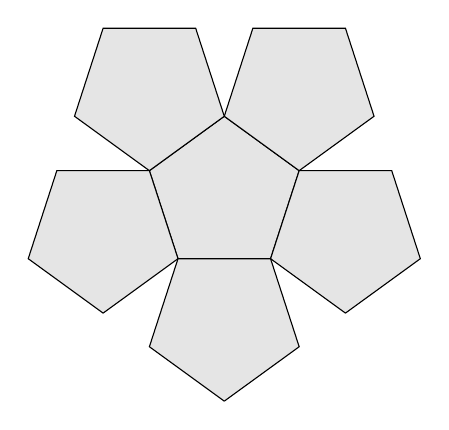
\begin{tikzpicture}
            \draw[fill=gray!20] (90:1)--(162:1)--(234:1)--(306:1)--(18:1)--(90:1);
            \foreach \i in {0,...,4}{
                \begin{scope}[shift = {(-18+72*\i :1.618)}]
                    \draw[fill=gray!20, rotate=180] (90:1)--(162:1)--(234:1)--(306:1)--(18:1)--(90:1);
                \end{scope}
            }
        \end{tikzpicture}
        \caption{Five-fold rotational symmetry is not compatible with translational symmetry.}
    \end{figure}

    Let's first see how various symmetry operators affect the diffraction patterns.
    \subsection{Symmetry Operations}
    \subsubsection{Inversion Centre}
    Suppose there is an inversion centre in the crystal, then by translational symmetry there must be one in each unit cell. We set it to be the origin of the unit cell, then for each atom at \((x_n,y_n,z_n)\), there must be the same atom at \((-x_n,-y_n,-z_n)\). Therefore, when calculating the structure factor, instead of summing over all \(N\) atoms in the unit cell, we can sum over the \(N/2\) pairs:
    \begin{align}
        F(hkl)&=\sum_{n=1}^{N/2}f_n\left[\exp[2\pi \ii(hx_n+ky_n+lz_n)]+\exp[-2\pi \ii(hx_n+ky_n+lz_n)]\right]\notag \\
        &=\sum_{n=1}^{N/2}2f_n\cos[2\pi (hx_n+ky_n+lz_n)]\,.\notag \\
        &=\sum_{n=1}^{N}f_n\cos[2\pi (hx_n+ky_n+lz_n)]\,.
    \end{align}
    Two immediate consequences are
    \begin{itemize}[topsep=0pt]
        \item The structure factor is always real (phase is \(0\) or \(\pi\)).
        \item \(F(hkl)=F(\bar{h}\bar{k}\bar{l})\).
    \end{itemize}
    Therefore, the structure factor also shows an inversion symmetry, with point group symmetry (at least) \(C_i\).

    However, this is not something we can really exploit. This is because we can only measure \(I(hkl)=\abs{F(hkl)}^2\), or equivalently the modulus of the structure factor.
    \begin{thm}[Friedel's law]
        For any crystal,
        \begin{equation}
            \abs{F(hkl)}=\abs{F(\bar{h}\bar{k}\bar{l})}\,.
        \end{equation}
    \end{thm}
    \begin{proof}
        This is because
        \begin{align}
            F(\bar{h}\bar{k}\bar{l})&=\sum_n f_n \exp[-2\pi \ii(hx_n+ky_n+lz_n)]\notag\\
            &=\left[\sum_n f_n\exp[2\pi \ii(hx_n+ky_n+lz_n)]\right]^*\notag\\
            &=F(hkl)^*\,.
        \end{align}
        They are complex conjugate, so they have the same modulus and diffraction intensity.\qed
    \end{proof}
    Therefore, the diffraction intensities of all crystals exhibit centres of inversion.

    In practice, when describing a diffraction pattern, we often picture a reciprocal lattice with its lattice points scaled by the intensity of diffraction. This construction is called the \textit{intensity-weighted reciprocal lattice}. The intensity-weighted reciprocal lattices of all crystals show a \(C_i\) point symmetry.

    \subsubsection*{Aside: Intensity Statistics}
    However, it is possible to infer the presence of an inversion centre from the diffraction pattern based on the intensities. If a centre of symmetry is not present, then generally \(F(hkl)\) would be a complex number, while if there is a centre of symmetry present, \(F(hkl)\) can only be a real number. A real \(F(hkl)\) has a higher probability to have a modulus close to zero than a complex one, and so we have a higher chance to observe weak \(F(hkl)\) values if an inversion centre is present.

    The above argument sounds a bit dubious. We can formalise it a little bit. Suppose the \(f_n\) values in a crystal follow some distribution with mean \(\mu\) and variance \(\sigma^2\), and the phase of each atom \(\phi_n\) is somehow random (uniformly distributed) between 0 and \(2\pi\).
    
    If there is a centre of inversion, then
    \begin{equation}
        F=\sum_n f_n\cos\phi_n\,.
    \end{equation}
    \(\cos\phi_n\) has a mean \(0\) and variance \(\frac{1}{2}\). By central limit theorem, if \(N\) is large, then \(F\) is a Gaussian with expectation value of
    \begin{equation}
        \mathbb{E}[F]=N \mathbb{E}[f_n\cos\phi_n]=N\mathbb{E}[f_n]\mathbb{E}[\cos\phi_n]=0
    \end{equation}
    and variance
    \begin{align}
        \Var[F]&=N\Var[f_n\cos\phi_n]\notag \\
        &=N\left[(\Var[f_n]+\mathbb{E}[f_n]^2)(\Var[\cos\phi_n]+\mathbb{E}[\cos\phi_n]^2)-\mathbb{E}[f_n]^2\mathbb{E}[\cos\phi_n]^2\right]\notag\\
        &=\frac{N}{2}(\sigma^2+\mu^2)\,.
    \end{align}
    Let's denote this variance \(\sigma_F^2\), then for the centrosymmetric case, the probability distribution function of \(\abs{F}\) is
    \begin{equation}
        g(x)=\frac{2}{\sigma_F\sqrt{2\pi}}\exp\left[-\frac{x^2}{2\sigma_F^2}\right]\,, \qquad x\ge 0\,.
    \end{equation}

    If there is not a symmetry of inversion, however, then
    \begin{equation}
        F=\sum_n f_n(\cos\phi_n+\ii\sin\phi_n)\,.
    \end{equation}
    The real and imaginary part of \(F\) then follows the same Gaussian distribution as the centrosymmetric case, with mean \(0\) and variance \(\sigma_F^2\). However, this is a 2D Gaussian. The probability density function of \(\abs{F}\) is then
    \begin{align}
        h(x)&=\int_{0}^{2\pi}\dd{\theta}x\frac{1}{2\pi \sigma_F^2}\exp\left[-\frac{x^2}{2\sigma_F^2}\right]\notag\\
        &=\frac{x}{\sigma_F^2}\exp\left[-\frac{x^2}{2\sigma_F^2}\right]\,.
    \end{align}
    Its probability density at 0 vanishes.

    \begin{figure}[ht!]
        \centering
        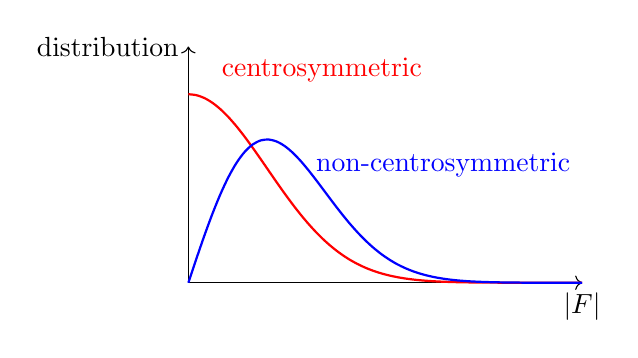
\begin{tikzpicture}
            \draw[->] (0,0)--(5,0)node[below]{\(\abs{F}\)};
            \draw[->] (0,0)--(0,3)node[left]{distribution};
            \draw[thick,domain=0:5, smooth, variable=\x,samples=50,red] plot ({\x}, {3*0.798*2.72^(-\x*\x/2)});
            \draw[thick,domain=0:5, smooth, variable=\x,samples=50,blue] plot ({\x}, {3*\x*2.72^(-\x*\x/2)});
            \node[red] at (0.3,2.7)[right]{centrosymmetric};
            \node[blue] at (1.5,1.5)[right]{non-centrosymmetric};
        \end{tikzpicture}
    \end{figure}

    \subsubsection{Mirror Plane}
    Consider a mirror plane perpendicular to the \(\vb{b}\) axis passing through the origin. This relates an atom at \((x,y,z)\) to another at \((x,-y,z)\). The structure factor can be simplified to
    \begin{align}
        F(hkl)&=\sum_{n=1}^{N/2}f_n[\exp[2\pi \ii(hx_n+ky_n+lz_n)]+\exp[2\pi \ii(hx_n-ky_n+lz_n)]]\notag \\
        &=\sum_{n=1}^{N}f_n\cos(2\pi ky_n)\exp[2\pi \ii(hx_n+lz_n)]\,.
    \end{align}
    Cosine is an even function, so
    \begin{equation}
        F(hkl)=F(h\bar{k}l)\,,
    \end{equation}
    and \(\abs{F(hkl)}^2=\abs{F(h\bar{k}l)}^2\). Therefore intensity-weighted reciprocal lattice will also have a mirror plane perpendicular to the \(\vb{b}^*\) axis. Combined with the \(i\) symmetry of Friedel pairs, we have
    \begin{equation}
        \abs{F(hkl)}^2=\abs{F(h\bar{k}l)}^2=\abs{F(\bar{h}k\bar{l})}^2=\abs{F(\bar{h}\bar{k}\bar{l})}^2\,,
    \end{equation}
    and so the intensity-weighted reciprocal lattice will have a \(C_{2h}\) symmetry. Note that \(i\) and \(\sigma_h\) generate the \(C_2\) symmetry.

    \begin{figure}
        \centering
        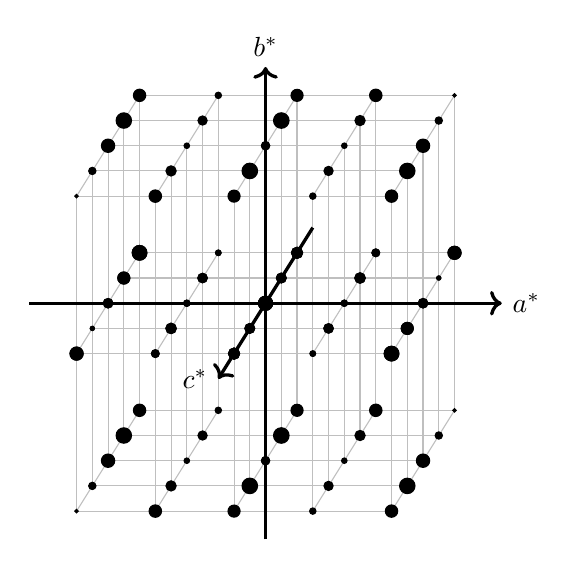
\begin{tikzpicture}[x={(1cm,0cm)},y={(0cm,1cm)},z={(-0.2cm,-0.32cm)}]
            \foreach \i in {-2,...,2}{
                \foreach \j in {-2,...,2}{
                    \draw[gray!50] (\i,-2,\j)--(\i,2,\j);
                }
                \foreach \j in {-1,0,1}{
                    \draw[gray!50] (\i,2*\j,-2)--(\i,2*\j,2);
                    \draw[gray!50] (-2,2*\j,\i)--(2,2*\j,\i);
                }
            }
            \foreach \i in {0,...,2}{
                \foreach \j in {0,1}{
                    \foreach \k in {-2,...,2}{
                        \tikzmath{\x = rand*0.04+0.06;}
                        \draw[fill=black] (\i,2*\j,\k) circle (\x);
                        \draw[fill=black] (\i,-2*\j,\k) circle (\x);
                        \draw[fill=black] (-\i,2*\j,-\k) circle (\x);
                        \draw[fill=black] (-\i,-2*\j,-\k) circle (\x);
                    }
                }
            }
            \draw[very thick,->] (-3,0,0)--(3,0,0)node[right]{\(a^*\)};
            \draw[very thick,->] (0,-3,0)--(0,3,0)node[above]{\(b^*\)};
            \draw[very thick,->] (0,0,-3)--(0,0,3)node[left]{\(c^*\)};
        \end{tikzpicture}
        \caption{An intensity-weighted reciprocal lattice with \(C_{2h}\) symmetry.}
    \end{figure}

    \subsubsection{Rotation Axes}
    Now let's consider the effect of a rotation axis. A \(m\)-fold rotation axis will rotate atoms by \(2\pi/m\) radians around the defined axis. For simplicity, we will only consider the 2-fold axis. We set the axis such that the rotation axis passes through the origin and is parallel to the \(\vb{b}\) axis of the unit cell, so that for each atom at \((x_n,y_n,z_n)\), there is also a same atom at \((-x,y,-z)\). In this case, we may simplify the structure factor to
    \begin{align}
        F(hkl)&=\sum_{n}^{N/2}f_n[\exp[2\pi \ii(hx_n+ky_n+lz_n)]+\exp[2\pi \ii(-hx_n+ky_n-lz_n)]]\notag \\
        &=\sum_{n}^{N}f_n\cos[2\pi(hx_n+lz_n)]\exp[2\pi \ii ky_n]\,.
    \end{align}
    Therefore,
    \begin{equation}
        F(hkl)=F(\bar{h}k\bar{l})\,.
    \end{equation}
    The intensity-weighted reciprocal lattice therefore also has a 2-fold rotation axis along \(\vb{b}^*\). Again, the Friedel's law still applies, so
    \begin{equation}
        \abs{F(hkl)}^2=\abs{F(h\bar{k}l)}^2=\abs{F(\bar{h}k\bar{l})}^2=\abs{F(\bar{h}\bar{k}\bar{l})}^2\,.
    \end{equation}
    Therefore the intensity-weighted reciprocal lattice has a \(C_{2h}\) point group symmetry (formally known as the \textit{Laue group}), as \(i\) and \(C_2\) further generates a \(\sigma_h\) symmetry.

    Finally, note that if a crystal structure exhibits a 2-fold rotation axis along one direction, or a mirror plane perpendicular to some direction, this axis must be perpendicular to two of the lattice vectors, otherwise the rotated cell will have a different orientation, and the translational symmetry will be broken. For example, if a 2-fold axis is parallel to \(\vb{b}\), then \(\vb{b}\) must be perpendicular to both \(\vb{a}\) and \(\vb{c}\). This means that the structure is at least \textit{monoclinic}, meaning that two of the unit-cell angles must be \(90^\circ\). By convention, we usually choose \(\alpha=\gamma=90^\circ\) and \(\beta\ne 90^\circ\) (although it could be that \(\beta=90^\circ\), but then we will classify the crystal to have a higher symmetry e.g. \textit{orthorhombic}).

    \subsubsection{Screw Axes}
    The fact that crystals are infinitely extended through the space leads us to some extra symmetry elements that are not present in point groups. Specifically, we can combine rotations or reflections with translations.

    A \(n_m\)-screw axis stands for a rotation of \(2\pi/n\) around the axis, and then a translation of \(m/n\) times the length of the lattice vector in that direction. We will only consider the 2-fold screw axis \(2_1\), and we will make the axis coincide with the \(\vb{b}\) vector. This is a rotation of \(180^\circ\) along \(\vb{b}\), and then translate by \(\vb{b}/2\), relating \((x,y,z)\) to \((-x,\frac{1}{2}+y,-z)\). The resulting structure factor is
    \begin{align}
        F(hkl)&=\sum_{n=1}^{N/2}f_n\exp(2\pi \ii ky_n)[\exp[2\pi \ii(hx_n+lz_n)]+(-1)^k\exp[-2\pi \ii(hx_n+lz_n)]]\notag \\
        &=\sum_{n=1}^{N}f_n\exp(2\pi \ii ky_n)\times\begin{cases}
            \cos[2\pi(hx_n+lz_n)] & \text{if \(k\) is even} \\
            \ii\sin[2\pi(hx_n+lz_n)] & \text{if \(k\) is odd.}
        \end{cases}
    \end{align}
    Consequently,
    \begin{equation}
        F(hkl)=\begin{cases}
            F(\bar{h}k\bar{l}) & \text{if \(k\) is even} \\
            -F(\bar{h}k\bar{l}) & \text{if \(k\) is odd,}
        \end{cases}
    \end{equation}
    but in either case,
    \begin{equation}
        \abs{F(hkl)}^2=\abs{F(\bar{h}k\bar{l})}^2\,.
    \end{equation}
    Combining with the Friedel pair relationship, we see that the \(2_1\) screw axis has exactly the same effect on the symmetry of the diffracted intensity as the 2-fold rotation axis, both having \(C_{2h}\).

    Moreover, if we consider the special case of \(h=l=0\), then the structure factor for \(0k0\) reduces to
    \begin{equation}
        F(0k0)=\sum_{n}^{N/2}f_n\exp(2\pi \ii ky_n)[1+(-1)^k]=\begin{cases}
            \sum_{n}^{N}f_n\exp(2\pi \ii ky_n) & \text{if \(k\) is even} \\
            0 & \text{if \(k\) is odd.}
        \end{cases}
    \end{equation}
    The structure factors for all \(0k0\) beams are zero if \(k\) is odd --- this result is independent of the atomic coordinates and is purely originates from symmetry. This is known as a \textit{systematic absence}. The pattern of the systematic absence depends on the direction of the screw axis:
    \begin{itemize}[topsep=0pt]
        \item \(2_1\) axis parallel to \(\vb{a}\): \((h00)\) absent for odd \(h\).
        \item \(2_1\) axis parallel to \(\vb{b}\): \((0k0)\) absent for odd \(k\).
        \item \(2_1\) axis parallel to \(\vb{c}\): \((00l)\) absent for odd \(l\).
    \end{itemize}

    We have a good explanation for this. Consider a \(2_1\) axis along \(\vb{b}\). If we project the 3D crystal structure into one dimension along \(\vb{b}\), i.e. we ignore the \(x\) and \(z\) coordinates, the presence of a \(2_1\) screw axis doubles the periodicity along \(\vb{b}\) direction, and hence the periodicity in the reciprocal lattice will be halved. This is exactly what a \(0k0\) beam is detecting: as reflections from a \((0k0)\) Bragg's plane has contributions from all \(x\) and \(z\) coordinates for a certain \(y\) value, it is only able to tell the periodicity along \(y\) direction, and it finds that things are repeating twice as often.

    \subsubsection{Glide Planes}
    A glide plane is a mirror plane reflection followed by a translation one half of the lattice. We will consider a \(c\)-glide perpendicular to \(b\), which is a reflection about a mirror plane perpendicular to \(b\) followed by a translation of \(\frac{1}{2}\vb{c}\), relating atoms at \((x,y,z)\) and \((x,-y,\frac{1}{2}+z)\). The structure factor equation becomes
    \begin{align}
        F(hkl)&=\sum_{n}^{N/2}f_n\exp[2\pi \ii(hx_n+lz_n)][\exp(2\pi \ii ky_n)+(-1)^l\exp(-2\pi \ii ky_n)]\notag \\
        &=\sum^{N}f_n\exp[2\pi \ii(hx_n+lz_n)]\times\begin{cases}
            \cos(2\pi ky_n) & \text{if \(l\) is even} \\
            \ii\sin(2\pi ky_n) & \text{if \(l\) is odd.}
        \end{cases}
    \end{align}
    This means that
    \begin{equation}
        F(hkl)=\begin{cases}
            F(h\bar{k}l) & \text{if \(l\) is even} \\
            -F(h\bar{k}l) & \text{if \(l\) is odd,}
        \end{cases}
    \end{equation}
    but in either case,
    \begin{equation}
        \abs{F(hkl)}^2=\abs{F(h\bar{k}l)}^2\,.
    \end{equation}
    The glide plane produces a mirror plane in the diffraction pattern, just as a normal mirror plane would do, and combining with Friedel pair relation, the diffraction pattern again has a \(C_{2h}\) symmetry.

    Consider \(k=0\), the structure factor reduces to
    \begin{equation}
        F(h0l)=\begin{cases}
            \sum_{n}^{N}f_n\exp[2\pi \ii(hx_n+lz_n)] & \text{if \(l\) is even} \\
            0 & \text{if \(l\) is odd.}
        \end{cases}
    \end{equation}
    Therefore, a \(c\)-glide perpendicular to \(b\) produces systematic absences of \(F(h0l)\) for odd \(l\). We again have a good explanation for it: we set \(k\) to 0 so the beam is ignorant of us changing the \(y\) coordinate by reflection, and now the translation of \(\frac{1}{2}\vb{c}\) doubles the periodicity along the \(c\) direction, so the reciprocal lattice is doubled in length in that direction.
    
    To conclude the systematic absence for glide planes: \\
    \textit{Glide plane perpendicular to \(a\)}:
    \begin{itemize}[topsep=0pt]
        \item \(b\)-glide: \((0kl)\) absent if \(k\) odd.
        \item \(c\)-glide: \((0kl)\) absent if \(l\) odd.
        \item \(n\)-glide: \((0kl)\) absent if \(k+l\) odd. (\(n\)-glide means translation by a half in both \(y\) and \(z\) directions)
    \end{itemize}
    \textit{Glide plane perpendicular to \(b\)}:
    \begin{itemize}[topsep=0pt]
        \item \(a\)-glide: \((h0l)\) absent if \(h\) odd.
        \item \(c\)-glide: \((h0l)\) absent if \(l\) odd.
        \item \(n\)-glide: \((h0l)\) absent if \(h+l\) odd.
    \end{itemize}
    \textit{Glide plane perpendicular to \(c\)}:
    \begin{itemize}[topsep=0pt]
        \item \(a\)-glide: \((hk0)\) absent if \(h\) odd.
        \item \(b\)-glide: \((hk0)\) absent if \(k\) odd.
        \item \(n\)-glide: \((hk0)\) absent if \(h+k\) odd.
    \end{itemize}

    \begin{figure}
        \centering
        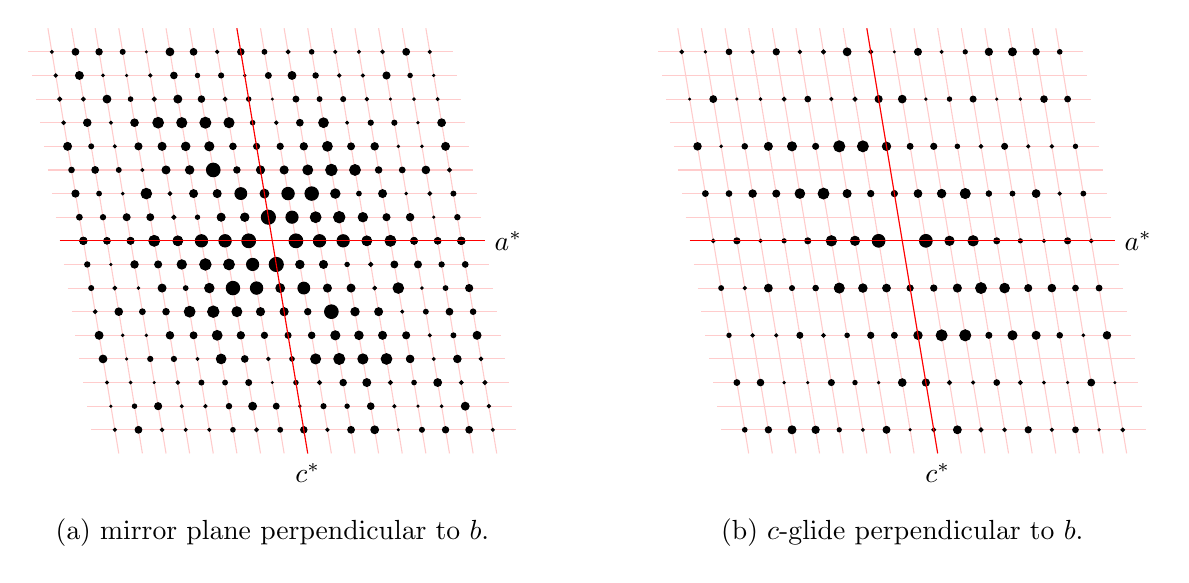
\begin{tikzpicture}
            \foreach \i in {-8,...,8}{
                \draw[thin,color=red!20] (-2.7-0.05*\i,0.3*\i)--(2.7-0.05*\i,0.3*\i);
                \draw[thin,color=red!20] (0.3*\i-0.45,2.7)--(0.3*\i+0.45,-2.7);
            }
            \foreach \i in {-8,...,8}{
                \foreach \j in {1,...,8}{
                    \tikzmath{\x = rand*0.02+0.03;
                    \y = rand*0.02+0.025;}
                    \draw[fill=black] (0.3*\i-0.05*\j,0.3*\j) circle (\x);
                    \draw[fill=black] (-0.3*\i+0.05*\j,-0.3*\j) circle (\x);
                    \draw[fill=black] (0.3*\j,0) circle (\y);
                    \draw[fill=black] (-0.3*\j,0) circle (\y);
                }
            }
            \foreach \i in {-3,...,3}{
                \foreach \j in {1,...,3}{
                    \tikzmath{\x = rand*0.04+0.05;
                    \y = rand*0.04+0.05;}
                    \draw[fill=black] (0.3*\i-0.05*\j,0.3*\j) circle (\x);
                    \draw[fill=black] (-0.3*\i+0.05*\j,-0.3*\j) circle (\x);
                    \draw[fill=black] (0.3*\j,0) circle (\y);
                    \draw[fill=black] (-0.3*\j,0) circle (\y);
                }
            }
            \foreach \i in {-5,...,5}{
                \foreach \j in {1,...,5}{
                    \tikzmath{\x = rand*0.03+0.04;
                    \y = rand*0.03+0.04;}
                    \draw[fill=black] (0.3*\i-0.05*\j,0.3*\j) circle (\x);
                    \draw[fill=black] (-0.3*\i+0.05*\j,-0.3*\j) circle (\x);
                    \draw[fill=black] (0.3*\j,0) circle (\y);
                    \draw[fill=black] (-0.3*\j,0) circle (\y);
                }
            }
            \draw[red] (-2.7,0)--(2.7,0)node[right,black]{\(a^*\)};
            \draw[red] (-0.45,2.7)--(0.45,-2.7)node[below,black]{\(c^*\)};
            \node at (0,-3.7) {(a) mirror plane perpendicular to \(b\).};

            \begin{scope}[shift={(8,0)}]
                \foreach \i in {-8,...,8}{
                    \draw[thin,color=red!20] (-2.7-0.05*\i,0.3*\i)--(2.7-0.05*\i,0.3*\i);
                    \draw[thin,color=red!20] (0.3*\i-0.45,2.7)--(0.3*\i+0.45,-2.7);
                }
                \foreach \i in {-8,...,8}{
                    \foreach \j in {1,...,4}{
                        \tikzmath{\x = rand*0.02+0.03;}
                        \draw[fill=black] (0.3*\i-0.1*\j,0.6*\j) circle (\x);
                        \draw[fill=black] (-0.3*\i+0.1*\j,-0.6*\j) circle (\x);
                    }
                }
                \foreach \i in {1,...,8}{
                    \tikzmath{\x = rand*0.02+0.03;}
                    \draw[fill=black] (0.3*\i,0) circle (\x);
                    \draw[fill=black] (-0.3*\i,0) circle (\x);
                }
                \foreach \i in {-3,...,3}{
                    \tikzmath{\x = rand*0.04+0.05;}
                    \draw[fill=black] (0.3*\i-0.1,0.6) circle (\x);
                    \draw[fill=black] (-0.3*\i+0.1,-0.6) circle (\x);
                }
                \foreach \i in {1,...,3}{
                    \tikzmath{\x = rand*0.04+0.05;}
                    \draw[fill=black] (0.3*\i,0) circle (\x);
                    \draw[fill=black] (-0.3*\i,0) circle (\x);
                }
                \foreach \i in {-5,...,5}{
                    \foreach \j in {2,4}{
                        \tikzmath{\x = rand*0.03+0.04;}
                        \draw[fill=black] (0.3*\i-0.05*\j,0.3*\j) circle (\x);
                        \draw[fill=black] (-0.3*\i+0.05*\j,-0.3*\j) circle (\x);
                    }
                }
                \foreach \i in {1,...,5}{
                    \tikzmath{\x = rand*0.03+0.04;}
                    \draw[fill=black] (0.3*\i,0) circle (\x);
                    \draw[fill=black] (-0.3*\i,0) circle (\x);
                }
                \draw[red] (-2.7,0)--(2.7,0)node[right,black]{\(a^*\)};
                \draw[red] (-0.45,2.7)--(0.45,-2.7)node[below,black]{\(c^*\)};
                \node at (0,-3.7) {(b) \(c\)-glide perpendicular to \(b\).};
            \end{scope}
        \end{tikzpicture}
        \caption{Schematic \((h0l)\) slices of the intensity-weighted reciprocal lattice. We see that glide planes create systematic absences, while mirror planes do not.}
    \end{figure}

    \subsection{Lattice Types}
    In some cases, it is more preferable to define a unit cell that is not primitive, i.e. containing more than one lattice point. This is possibly because the non-primitive unit cell has a higher symmetry, or it allows the symmetry elements to align with the axes of the unit cell.

    There are in total four types of 3D unit cells. The first type is \textit{primitive}, denoted \(P\), where the lattice points are at the corners of the cells only, so that there is only one lattice point in the unit cell. It is also possible for a cell to also contain lattice points in the centre of two opposite faces. This is conventionally chosen to be the \(ab\) face, so this type of cell is known as \textit{\(C\)-centred}. Another possibility is to contain a second lattice point at the centre of the cell, and this is known as \textit{body-centred} or \textit{\(I\)-centred}. Finally, we can have lattice points at the centres of all unit-cell faces, which is known as \textit{face-centred} or \textit{\(F\)-centred}.

    \begin{figure}
        \centering
        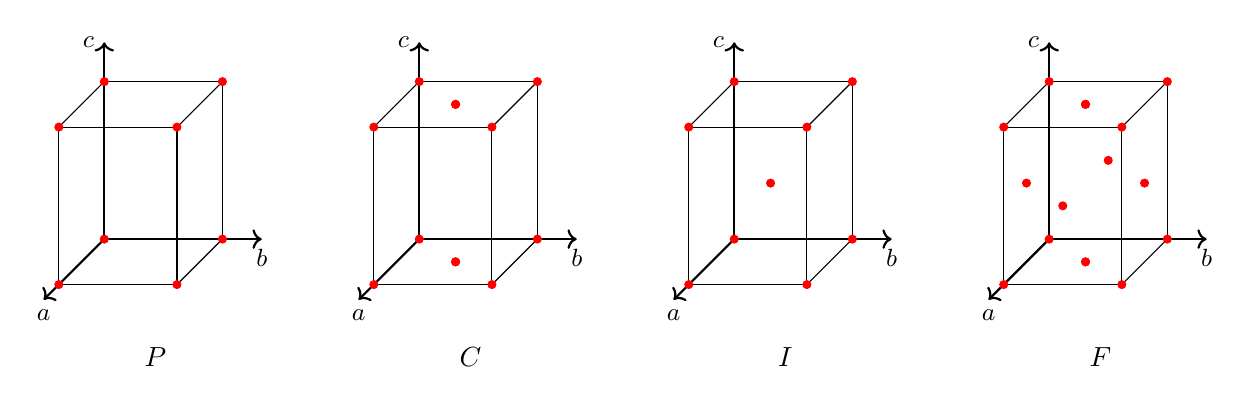
\begin{tikzpicture}
            \draw[->,thick] (0,0,0)--(0,0,2)node[below]{\small \(a\)};
            \draw[->,thick] (0,0,0)--(0,2.5,0)node[left]{\small \(c\)};
            \draw[->,thick] (0,0,0)--(2,0,0)node[below]{\small \(b\)};
            \foreach \i in {0,1.5}{
                \draw (0,0,\i) rectangle (1.5,2,\i);
                \foreach \j in {0,2}{
                    \draw (\i,\j,0) -- (\i,\j,1.5);
                }
            }
            \foreach \i in {0,1.5}{
                \foreach \j in {0,2}{
                    \foreach \k in {0,1.5}{
                        \draw[red,fill=red] (\i,\j,\k) circle (0.05);
                    }
                }
            }
            \node at (0.65,-1.5) {\(P\)};

            \begin{scope}[shift={(4,0)}]
                \draw[->,thick] (0,0,0)--(0,0,2)node[below]{\small \(a\)};
                \draw[->,thick] (0,0,0)--(0,2.5,0)node[left]{\small \(c\)};
                \draw[->,thick] (0,0,0)--(2,0,0)node[below]{\small \(b\)};
                \foreach \i in {0,1.5}{
                    \draw (0,0,\i) rectangle (1.5,2,\i);
                    \foreach \j in {0,2}{
                        \draw (\i,\j,0) -- (\i,\j,1.5);
                    }
                }
                \foreach \i in {0,1.5}{
                    \foreach \j in {0,2}{
                        \foreach \k in {0,1.5}{
                            \draw[red,fill=red] (\i,\j,\k) circle (0.05);
                        }
                        \draw[red,fill=red] (0.75,\j,0.75) circle (0.05);
                    }
                }
                \node at (0.65,-1.5) {\(C\)};
            \end{scope}

            \begin{scope}[shift={(8,0)}]
                \draw[->,thick] (0,0,0)--(0,0,2)node[below]{\small \(a\)};
                \draw[->,thick] (0,0,0)--(0,2.5,0)node[left]{\small \(c\)};
                \draw[->,thick] (0,0,0)--(2,0,0)node[below]{\small \(b\)};
                \foreach \i in {0,1.5}{
                    \draw (0,0,\i) rectangle (1.5,2,\i);
                    \foreach \j in {0,2}{
                        \draw (\i,\j,0) -- (\i,\j,1.5);
                    }
                }
                \foreach \i in {0,1.5}{
                    \foreach \j in {0,2}{
                        \foreach \k in {0,1.5}{
                            \draw[red,fill=red] (\i,\j,\k) circle (0.05);
                        }
                    }
                }
                \draw[red,fill=red] (0.75,1,0.75) circle (0.05);
                \node at (0.65,-1.5) {\(I\)};
            \end{scope}

            \begin{scope}[shift={(12,0)}]
                \draw[->,thick] (0,0,0)--(0,0,2)node[below]{\small \(a\)};
                \draw[->,thick] (0,0,0)--(0,2.5,0)node[left]{\small \(c\)};
                \draw[->,thick] (0,0,0)--(2,0,0)node[below]{\small \(b\)};
                \foreach \i in {0,1.5}{
                    \draw (0,0,\i) rectangle (1.5,2,\i);
                    \foreach \j in {0,2}{
                        \draw (\i,\j,0) -- (\i,\j,1.5);
                    }
                }
                \foreach \i in {0,1.5}{
                    \foreach \j in {0,2}{
                        \foreach \k in {0,1.5}{
                            \draw[red,fill=red] (\i,\j,\k) circle (0.05);
                        }
                        \draw[red,fill=red] (0.75,\j,0.75) circle (0.05);
                    }
                    \draw[red,fill=red] (\i,1,0.75) circle (0.05);
                    \draw[red,fill=red] (0.75,1,\i) circle (0.05);
                }
                \node at (0.65,-1.5) {\(F\)};
            \end{scope}
        \end{tikzpicture}
        \caption{Types of unit cell centring.}
    \end{figure}

    Since non-primitive unit cells contain more than one lattice points, they also have systematic absences, which can be worked out using the same way as we did before.
    \begin{itemize}[topsep=0pt]
        \item \(P\): No systematic absences.
        \item \(C\): \((hkl)\) absent if \(h+k=2n+1\).
        \item \(I\): \((hkl)\) absent if \(h+k+l=2n+1\).
        \item \(F\): \((hkl)\) absent unless \(h,k,l\) are all odd or all even.
    \end{itemize}
    Heuristically, the reciprocal lattice of a \(P\) and a \(C\) lattices are themselves, the reciprocal lattice of an \(I\) lattice is a larger \(F\) lattice, and the reciprocal lattice of an \(F\) lattice is a larger \(I\) lattice.

    By using a non-primitive cell, we are choosing to describe the real lattice with longer lattice vectors, so the reciprocal lattice vectors are correspondingly shorter. We are therefore using smaller reciprocal unit cells than a primitive reciprocal unit cell. Hence, systematic absences must arise.

    \subsection{Space Groups and Equivalent Positions}
    An identification of the lattice type together with a collection of symmetry operators defines a \textit{space group}. It describes the symmetry of a crystal, just as a point group describes the symmetry of a molecule, but we have an extra translational symmetry described by the lattice type.

    For example, let's consider the most common space group \(P2_1/c\), where its name stands for primitive lattice, a \(2_1\) screw axis \(\parallel b\) and a \(c\)-glide \(\perp b\). These symmetry elements also create a centre of inversion. By convention, we set the inversion centre to be the origin, so that the \(2_1\) axis is at \((0,y,1/4)\) and the \(c\)-glide is at \((x,1/4,z)\). This collection of symmetry operators produces a set of coordinates that are related to each other, known as the \textit{general equivalent positions} (GEPs). The GEPs for \(P2_1/c\) are shown in the figure below.

    \begin{figure}[ht!]
        \centering
        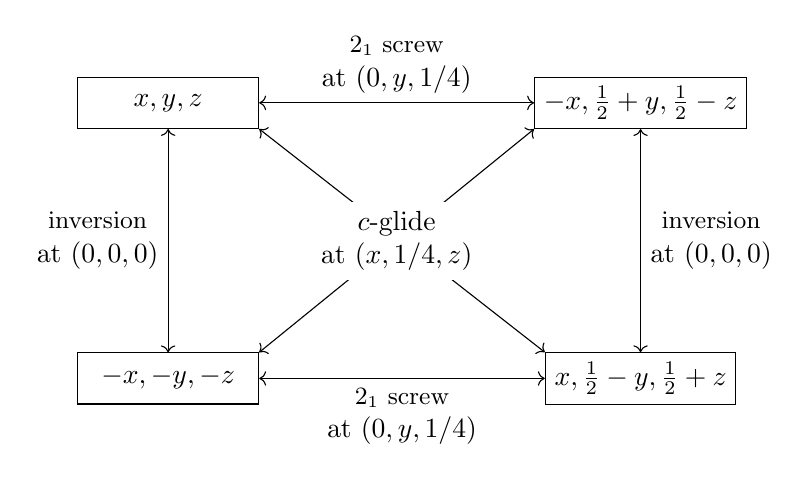
\begin{tikzpicture}
            \node[draw,minimum height=0.65cm,minimum width=2.3cm] (A) at (0,0){\(x,y,z\)};
            \node[draw,minimum height=0.65cm,minimum width=2.3cm] (B) at (6,0){\(-x,\frac{1}{2}+y,\frac{1}{2}-z\)};
            \node[draw,minimum height=0.65cm,minimum width=2.3cm] (C) at (0,-3.5){\(-x,-y,-z\)};
            \node[draw,minimum height=0.65cm,minimum width=2.3cm] (D) at (6,-3.5){\(x,\frac{1}{2}-y,\frac{1}{2}+z\)};
            \draw[<->] (A.east)--node[above,align=center]{\small \(2_1\) screw \\ at \((0,y,1/4)\)}(B.west);
            \draw[<->] (C.east)--node[below,align=center]{\small \(2_1\) screw \\ at \((0,y,1/4)\)}(D.west);
            \draw[<->] (A.south)--node[left,align=center]{\small inversion \\ at \((0,0,0)\)}(C.north);
            \draw[<->] (B.south)--node[right,align=center]{\small inversion \\ at \((0,0,0)\)}(D.north);
            \draw[<->] (A.south east)--(D.north west);
            \draw[<->] (C.north east)--node[fill=white,align=center]{\(c\)-glide \\ at \((x,1/4,z)\)}(B.south west);
        \end{tikzpicture}
        \caption{General equivalent positions in the \(P2_1/c\) space group.}
    \end{figure}

    Therefore, there exists a minimal set of atomic coordinates that need to be specified to describe the whole unit cell (and hence the entire crystal structure), which is known as the \textit{asymmetric unit}. The coordinates of the other atoms in the cell can be obtained by applying the symmetry elements in the space group.

    However, notice that there are some special coordinates in the \(P2_1/c\) group that do not produce a group of four distinct coordinates when the symmetry operators are applied. An example is \((0,0,0)\), for which you will only obtain two distinct coordinates \((0,0,0)\) and \((0,1/2,1/2)\) when applying the symmetry elements. Such positions are called the \textit{special equivalent positions}. They arise because the coordinates coincide with the point group elements (centre of symmetry in this case), so it is not moved by those symmetry elements. Similarly, if a rotation axis or a mirror plane is present in some space group, there will be a whole line and a whole plane of special equivalent positions, respectively.

    \begin{figure}
        \centering
        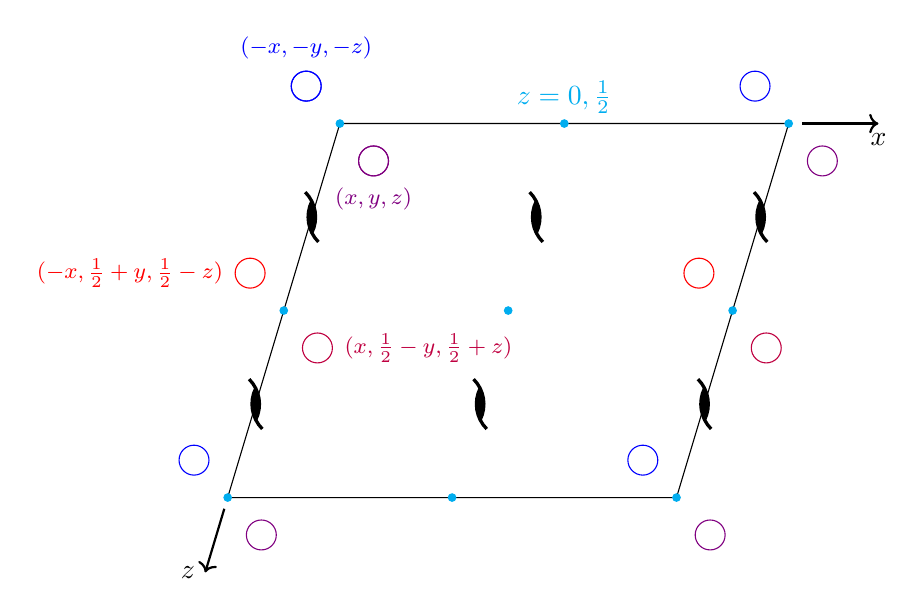
\begin{tikzpicture}[scale=0.95]
            \draw[x={(6cm,0cm)},y={(-1.5cm,-5cm)}] (0,0)--(1,0)--(1,1)--(0,1)--(0,0);
            \draw[x={(6cm,0cm)},y={(-1.5cm,-5cm)},thick,->] (1.03,0)--(1.2,0) node[below]{\(x\)};
            \draw[x={(6cm,0cm)},y={(-1.5cm,-5cm)},thick,->] (0,1.03)--(0,1.2) node[left]{\(z\)};
            \foreach \i in {0,1}{
                \foreach \j in {0,1,2}{
                    \pic at (-0.375+3*\j-0.75*\i,-1.25-2.5*\i) {screw};
                }
            }
            \foreach \i in {0,1,2}{
                \foreach \j in {0,1,2}{
                    \draw[cyan,fill=cyan] (3*\i-0.75*\j,-2.5*\j) circle (0.05);
                }
            }
            \node[cyan] at (3,0)[above]{\(z=0,\frac{1}{2}\)};
            \draw[violet] (0.45,-0.5)node[below=0.22 cm]{\footnotesize\((x,y,z)\)} circle (0.2);
            \draw[blue] (-0.45,0.5)node[above=0.22 cm]{\footnotesize\((-x,-y,-z)\)} circle (0.2);
            \draw[red] (-1.2,-2)node[left=0.22 cm]{\footnotesize\((-x,\frac{1}{2}+y,\frac{1}{2}-z)\)} circle (0.2);
            \draw[purple] (-0.3,-3)node[right=0.22 cm]{\footnotesize\((x,\frac{1}{2}-y,\frac{1}{2}+z)\)} circle (0.2);
            \foreach \i in {0,1}{
                \foreach \j in {0,1}{
                    \draw[violet] (0.45+6*\i-1.5*\j,-0.5-5*\j) circle (0.2);
                    \draw[blue] (-0.45+6*\i-1.5*\j,0.5-5*\j) circle (0.2);
                }
            }
            \draw[red] (4.8,-2) circle (0.2);
            \draw[purple] (5.7,-3) circle (0.2);
        \end{tikzpicture}
        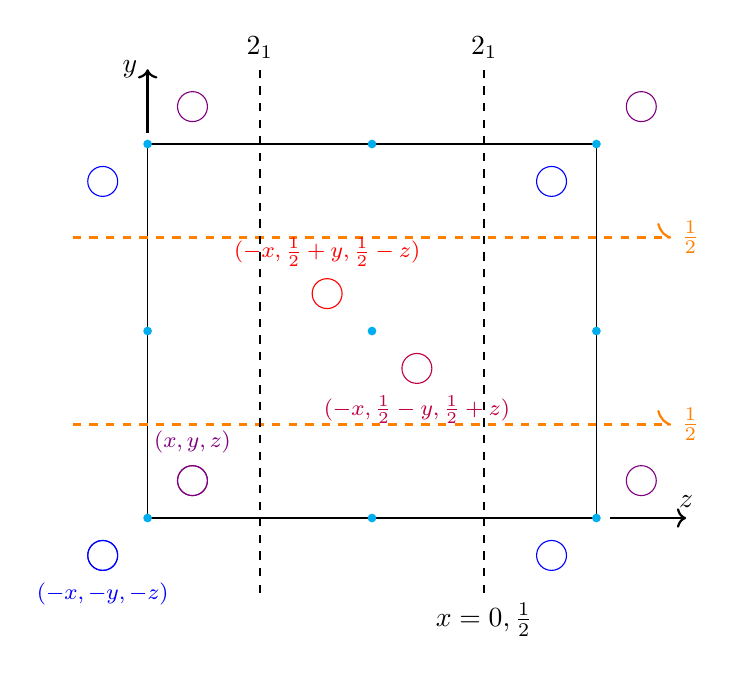
\begin{tikzpicture}[scale=0.95]
            \draw (0,0) rectangle (6,5);
            \draw[thick,->] (6.18,0)--(7.2,0)node[above]{\(z\)};
            \draw[thick,->] (0,5.15)--(0,6)node[left]{\(y\)};
            \draw[thick,dashed,orange,arrows = {->[harpoon,scale=1.5]}] (-1,1.25)--(7,1.25)node[right]{\(\frac{1}{2}\)};
            \draw[thick,dashed,orange,arrows = {->[harpoon,scale=1.5]}] (-1,3.75)--(7,3.75)node[right]{\(\frac{1}{2}\)};
            \draw[dashed,thick] (1.5,-1)--(1.5,6)node[above]{\(2_1\)};
            \foreach \i in {0,1,2}{
                \foreach \j in {0,1,2}{
                    \draw[cyan,fill=cyan] (3*\i,2.5*\j) circle (0.05);
                }
            }
            \draw[dashed,thick] (4.5,-1)node[below]{\(x=0,\frac{1}{2}\)}--(4.5,6)node[above]{\(2_1\)};
            \draw[blue] (-0.6,-0.5)node[below=0.22 cm]{\footnotesize\((-x,-y,-z)\)} circle (0.2);
            \draw[violet] (0.6,0.5)node[above=0.22 cm]{\footnotesize\((x,y,z)\)} circle (0.2);
            \draw[red] (2.4,3)node[above=0.22 cm]{\footnotesize\((-x,\frac{1}{2}+y,\frac{1}{2}-z)\)} circle (0.2);
            \draw[purple] (3.6,2)node[below=0.22 cm]{\footnotesize\((-x,\frac{1}{2}-y,\frac{1}{2}+z)\)} circle (0.2);
            \foreach \i in {0,1}{
                \foreach \j in {0,1}{
                    \draw[blue] (-0.6+6*\i,-0.5+5*\j) circle (0.2);
                    \draw[violet] (0.6+6*\i,0.5+5*\j) circle (0.2);
                }
            }
        \end{tikzpicture}
        \caption{View of \(P2_1/c\) space group unit cell along \(y\) axis and \(x\) axis. Note that extra symmetry elements arise automatically such that they appear twice as often as the lattice points.}
    \end{figure}

    \subsection{Determining Space Group}
    Having obtained a diffraction pattern from the experiment, we should be able to easily determine the space group. First, by observing the reciprocal cell geometry, we should be able to infer the lattice vectors \(a\), \(b\), \(c\) and their angles \(\alpha\), \(\beta\) and \(\gamma\). Then by observing the general \((hkl)\) systematic absences, we can infer the lattice type (\(P\), \(I\), \(F\) or \(C\)). This will give us one of the 14 possible types of 3D lattice, known as the \textit{Bravais lattices}.

    \begin{table}[ht!]
        \centering
        \caption{The 14 Bravais lattices.}
        \begin{tabular}{ccccc}
            \toprule
            Crystal system & \(P\) & \(I\) & \(F\) & \(C\) \\ \midrule
            \makecell{\(\) \\ Cubic \\ \(a=b=c\) \\
            \(\alpha=\beta=\gamma=90^\circ\) \\ \(\)} & \raisebox{-0.42\totalheight}{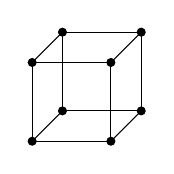
\begin{tikzpicture}
                \foreach \i in {0,1}{
                    \foreach \j in {0,1}{
                        \foreach \k in {0,1}{
                            \draw[fill=black] (\i,\j,\k) circle (0.05);
                        }
                        \draw (\i,\j,0)--(\i,\j,1);
                    }
                    \draw (0,0,\i) rectangle (1,1,\i);
                }
            \end{tikzpicture}} & \raisebox{-0.42\totalheight}{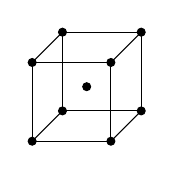
\begin{tikzpicture}
                \foreach \i in {0,1}{
                    \foreach \j in {0,1}{
                        \foreach \k in {0,1}{
                            \draw[fill=black] (\i,\j,\k) circle (0.05);
                        }
                        \draw (\i,\j,0)--(\i,\j,1);
                    }
                    \draw (0,0,\i) rectangle (1,1,\i);
                }
                \draw[fill=black] (0.5,0.5,0.5) circle (0.05);
            \end{tikzpicture}} & \raisebox{-0.42\totalheight}{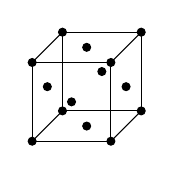
\begin{tikzpicture}
                \foreach \i in {0,1}{
                    \foreach \j in {0,1}{
                        \foreach \k in {0,1}{
                            \draw[fill=black] (\i,\j,\k) circle (0.05);
                        }
                        \draw (\i,\j,0)--(\i,\j,1);
                    }
                    \draw (0,0,\i) rectangle (1,1,\i);
                    \draw[fill=black] (0.5,0.5,\i) circle (0.05);
                    \draw[fill=black] (0.5,\i,0.5) circle (0.05);
                    \draw[fill=black] (\i,0.5,0.5) circle (0.05);
                }
            \end{tikzpicture}} \\ \midrule
            \makecell{\(\) \\ Tetragonal \\
            \(a=b\ne c\) \\
            \(\alpha=\beta=\gamma=90^\circ\) \\ \(\)} & \raisebox{-0.45\totalheight}{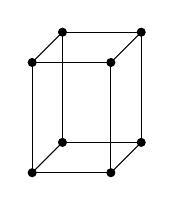
\begin{tikzpicture}
                \foreach \i in {0,1}{
                    \foreach \j in {0,1}{
                        \foreach \k in {0,1}{
                            \draw[fill=black] (\i,1.4*\j,\k) circle (0.05);
                        }
                        \draw (\i,1.4*\j,0)--(\i,1.4*\j,1);
                    }
                    \draw (0,0,\i) rectangle (1,1.4,\i);
                }
            \end{tikzpicture}} & \raisebox{-0.45\totalheight}{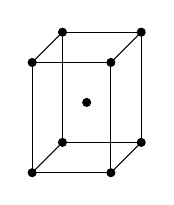
\begin{tikzpicture}
                \foreach \i in {0,1}{
                    \foreach \j in {0,1}{
                        \foreach \k in {0,1}{
                            \draw[fill=black] (\i,1.4*\j,\k) circle (0.05);
                        }
                        \draw (\i,1.4*\j,0)--(\i,1.4*\j,1);
                    }
                    \draw (0,0,\i) rectangle (1,1.4,\i);
                }
                \draw[fill=black] (0.5,0.7,0.5) circle (0.05);
            \end{tikzpicture}} \\ \midrule
            \makecell{\(\) \\ Orthorhombic \\
            \(a\ne b\ne c\) \\
            \(\alpha=\beta=\gamma=90^\circ\) \\ \(\)} & \raisebox{-0.45\totalheight}{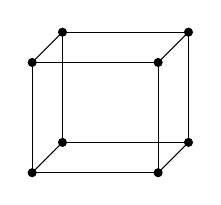
\begin{tikzpicture}
                \foreach \i in {0,1}{
                    \foreach \j in {0,1}{
                        \foreach \k in {0,1}{
                            \draw[fill=black] (1.6*\i,1.4*\j,\k) circle (0.05);
                        }
                        \draw (1.6*\i,1.4*\j,0)--(1.6*\i,1.4*\j,1);
                    }
                    \draw (0,0,\i) rectangle (1.6,1.4,\i);
                }
            \end{tikzpicture}} & \raisebox{-0.45\totalheight}{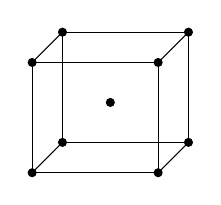
\begin{tikzpicture}
                \foreach \i in {0,1}{
                    \foreach \j in {0,1}{
                        \foreach \k in {0,1}{
                            \draw[fill=black] (1.6*\i,1.4*\j,\k) circle (0.05);
                        }
                        \draw (1.6*\i,1.4*\j,0)--(1.6*\i,1.4*\j,1);
                    }
                    \draw (0,0,\i) rectangle (1.6,1.4,\i);
                }
                \draw[fill=black] (0.8,0.7,0.5) circle (0.05);
            \end{tikzpicture}} & \raisebox{-0.45\totalheight}{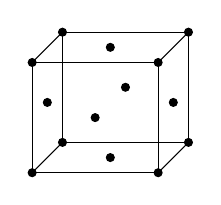
\begin{tikzpicture}
                \foreach \i in {0,1}{
                    \foreach \j in {0,1}{
                        \foreach \k in {0,1}{
                            \draw[fill=black] (1.6*\i,1.4*\j,\k) circle (0.05);
                        }
                        \draw (1.6*\i,1.4*\j,0)--(1.6*\i,1.4*\j,1);
                    }
                    \draw (0,0,\i) rectangle (1.6,1.4,\i);
                    \draw[fill=black] (0.8,0.7,\i) circle (0.05);
                    \draw[fill=black] (0.8,1.4*\i,0.5) circle (0.05);
                    \draw[fill=black] (1.6*\i,0.7,0.5) circle (0.05);
                }
            \end{tikzpicture}} & \raisebox{-0.45\totalheight}{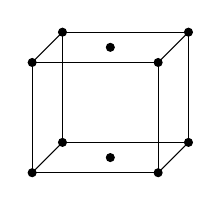
\begin{tikzpicture}
                \foreach \i in {0,1}{
                    \foreach \j in {0,1}{
                        \foreach \k in {0,1}{
                            \draw[fill=black] (1.6*\i,1.4*\j,\k) circle (0.05);
                        }
                        \draw (1.6*\i,1.4*\j,0)--(1.6*\i,1.4*\j,1);
                    }
                    \draw (0,0,\i) rectangle (1.6,1.4,\i);
                    \draw[fill=black] (0.8,1.4*\i,0.5) circle (0.05);
                }
            \end{tikzpicture}} \\ \midrule
            \makecell{\(\) \\ Hexagonal \\
            \(a=b\ne c\) \\
            \(\alpha=\beta=90^\circ\), \(\gamma=120^\circ\) \\ \(\)} & \raisebox{-0.45\totalheight}{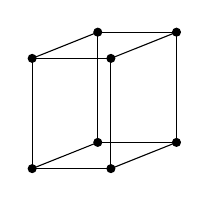
\begin{tikzpicture}[z={(-0.833cm,-0.333cm)}]
                \foreach \i in {0,1}{
                    \foreach \j in {0,1}{
                        \foreach \k in {0,1}{
                            \draw[fill=black] (\i,1.4*\j,\k) circle (0.05);
                        }
                        \draw (\i,1.4*\j,0)--(\i,1.4*\j,1);
                    }
                    \draw (0,0,\i) rectangle (1,1.4,\i);
                }
            \end{tikzpicture}} \\ \midrule
            \makecell{\(\) \\ Trigonal \\
            \(a=b=c\) \\
            \(\alpha=\beta=\gamma\ne 90^\circ\) \\ \(\)} & \raisebox{-0.45\totalheight}{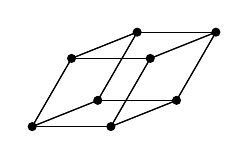
\begin{tikzpicture}
                \foreach \i in {0,1}{
                    \foreach \j in {0,1}{
                        \foreach \k in {0,1}{
                            \draw[fill=black] (\i+0.5*\j-0.5*\k,0.866*\j,0.866*\k) circle (0.05);
                            \draw (0.5*\j-0.5*\k,0.866*\j,0.866*\k)--(1+0.5*\j-0.5*\k,0.866*\j,0.866*\k);
                            \draw (\i-0.5*\k,0,0.866*\k)--(\i+0.5-0.5*\k,0.866,0.866*\k);
                            \draw (\i+0.5*\j,0.866*\j,0)--(\i+0.5*\j-0.5,0.866*\j,0.866);
                        }
                    }
                }
            \end{tikzpicture}} \\ \midrule
            \makecell{\(\) \\ Monoclinic \\
            \(a\ne b\ne c\) \\
            \(\alpha=\gamma=90^\circ\), \(\beta\ne 90^\circ\) \\ \(\)} & \raisebox{-0.45\totalheight}{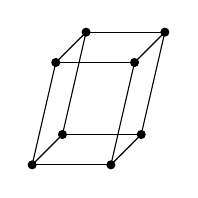
\begin{tikzpicture}
                \foreach \i in {0,1}{
                    \foreach \j in {0,1}{
                        \foreach \k in {0,1}{
                            \draw[fill=black] (\i+0.3*\j,1.3*\j,\k) circle (0.05);
                        }
                        \draw (\i+0.3*\j,1.3*\j,0)--(\i+0.3*\j,1.3*\j,1);
                        \draw (\i,0,\j)--(\i+0.3,1.3,\j);
                        \draw (0.3*\i,1.3*\i,\j)--(1+0.3*\i,1.3*\i,\j);
                    }
                }
            \end{tikzpicture}} & & & \raisebox{-0.45\totalheight}{\begin{tikzpicture}
                \foreach \i in {0,1}{
                    \foreach \j in {0,1}{
                        \foreach \k in {0,1}{
                            \draw[fill=black] (\i+0.3*\j,1.3*\j,\k) circle (0.05);
                        }
                        \draw (\i+0.3*\j,1.3*\j,0)--(\i+0.3*\j,1.3*\j,1);
                        \draw (\i,0,\j)--(\i+0.3,1.3,\j);
                        \draw (0.3*\i,1.3*\i,\j)--(1+0.3*\i,1.3*\i,\j);
                    }
                    \draw[fill=black] (0.5+0.3*\i,1.3*\i,0.5) circle (0.05);
                }
            \end{tikzpicture}} \\ \midrule
            \makecell{\(\) \\ Triclinic \\
            \(a\ne b\ne c\) \\
            \(\alpha\ne \beta\ne \gamma\ne 90^\circ\) \\ \(\)} & \raisebox{-0.45\totalheight}{\begin{tikzpicture}
                \foreach \i in {0,1}{
                    \foreach \j in {0,1}{
                        \foreach \k in {0,1}{
                            \draw[fill=black] (\i+0.2*\j-0.4*\k,1.3*\j,0.9*\k) circle (0.05);
                            \draw (0.2*\j-0.4*\k,1.3*\j,0.9*\k)--(1+0.2*\j-0.4*\k,1.3*\j,0.9*\k);
                            \draw (\i-0.4*\k,0,0.9*\k)--(\i+0.2-0.4*\k,1.3,0.9*\k);
                            \draw (\i+0.2*\j,1.3*\j,0)--(\i+0.2*\j-0.4,1.3*\j,0.9);
                        }
                    }
                }
            \end{tikzpicture}} \\ \bottomrule
        \end{tabular}
    \end{table}

    Having determined the lattice type, we can then identify the symmetry elements in the crystal. If the intensity-weighted reciprocal lattice exhibits a \(C_{2h}\) symmetry, then there will be a \(C_2\) axis or a mirror plane in the structure. If there are other systematic absences, then there will be glide planes or screw axes. We can identify the presence of inversion centres from intensity statistics.

    In practice, this can be easily done using automated programs. However, for a genuine experiment, there will be measurement errors, or there might be ambiguity on whether a diffraction is too small or it is really absent. Hence, all of these assessment indicate probable space groups rather than a concrete assessment.

    \subsection{Symmetry in Patterson Functions}
    Symmetry also allows us to identify atomic coordinates directly from Patterson function. Suppose we have confirmed that a crystal has a space group \(P2_1/c\) from diffraction pattern, we then know that the crystal must have the same atom at the following general equivalent positions:
    \begin{align*}
        (a):&\ (x,y,z) & (b):&\ \textstyle (-x,\frac{1}{2}+y,\frac{1}{2}-z) & (c):&\ \textstyle (x,\frac{1}{2}-y,\frac{1}{2}+z) & (d):&\ (-x,-y,-z)\,.
    \end{align*}
    This results in 16 interatomic vectors in the Patterson function: four of them are self-vectors at the origin, and the remaining twelve are non-origin vectors. Since each \(A\to B\) vector will be accompanied by a \(A\leftarrow B\) in reverse, these will comprise six centrosymmetric pairs:
    \begin{enumerate}[topsep=0pt,label=(\roman*)]
        \item \((a)\leftrightarrow (b)\): \(\pm (2x,-\frac{1}{2},-\frac{1}{2}+2z)\),
        \item \((a)\leftrightarrow (c)\): \(\pm (0,-\frac{1}{2}+2y,-\frac{1}{2})\),
        \item \((a)\leftrightarrow (d)\): \(\pm (2x,2y,2z)\),
        \item \((b)\leftrightarrow (c)\): \(\pm (-2x,2y,-2z)\),
        \item \((b)\leftrightarrow (d)\): \(\pm (0,\frac{1}{2}+2y,\frac{1}{2})\),
        \item \((c)\leftrightarrow (d)\): \(\pm (2x,\frac{1}{2},\frac{1}{2}+2z)\).
    \end{enumerate}
    As the structure is periodic, there will be the same atom 1 unit away along any coordinate, so we can shift any coordinate by \(\pm 1\). Consequently, vector (i) is actually identical to (vi), and (ii) is identical to (v). Therefore, for the space group \(P2_1/c\), we actually have two pairs of doubly-weighted peaks at \(\pm (2x,\frac{1}{2},\frac{1}{2}+2z)\), \(\pm (0,\frac{1}{2}+2y,\frac{1}{2})\) and two pairs of singly-weighted peaks at \(\pm(2x,2y,2z)\) and \(\pm(-2x,2y,-2z)\). Those peaks in the Patterson functions are easy to locate because of their special forms (0 or \(\frac{1}{2}\) in some coordinates). By identifying the coordinates of these peaks in the Patterson function, we can directly work out the coordinates of these atoms.

    Note that since the Patterson function only gives distinct peaks for interatomic vectors between heavy atoms, this usually only allow us to work out the coordinates of the heavy atoms in the structure. However, this is usually a very important first step for a complete structure determination. Having known this initial information, we have three complementary methods to determine the coordinates of the rest of the atoms. They are the \textit{heavy atom method}, \textit{isomorphous replacement} and \textit{anomalous scattering}.

    \subsection{The Heavy Atom Method}
    Suppose of the \(N\) atoms in the unit cell, we know the coordinate of the \(M\) heavy atoms of them e.g. from Patterson function. We can split the structure factor into a contribution of heavy atoms and the contribution of the rest of the atoms.
    \begin{align}
        F(hkl)&=\sum_{n=1}^{N}f_n \exp[2\pi \ii(hx_n+ky_n+lz_n)]\notag\\
        &=\sum_{n\text{ heavy}}f_n \exp[2\pi \ii(hx_n+ky_n+lz_n)] + \sum_{n\text{ rest}}f_n \exp[2\pi \ii(hx_n+ky_n+lz_n)]\notag\\
        &=F_{\text{heavy}}(hkl)+F_{\text{rest}}(hkl)\,.
    \end{align}
    From experiment, we can only measure \(\abs{F(hkl)}\), not \(\Phi(hkl)\). But since we know the coordinate of the \(M\) heavy atoms, we can calculate
    \begin{equation}
        F_{\text{heavy}}=\sum_{n=1}^{M}f_n \exp[2\pi \ii(hx_n+ky_n+lz_n)]\,.
    \end{equation}
    In particular, we know both the amplitude and the phase of the heavy atom contribution. Since the diffracting power of an atom \(f_n\), is proportional to the number of electrons, which is in turn proportional to the atomic number, heavy atom contributions tend to dominate in \(F(hkl)\).
    \[\abs{F_{\text{heavy}}(hkl)}\stackrel{?}{\gg}\abs{F_{\text{rest}}(hkl)}\,.\]
    This allows us to argue that hopefully \(\Phi(hkl)\) is close to \(\Phi_{\text{heavy}}(hkl)\), so we can use it as an estimate of \(\Phi(hkl)\). This allows us to combine the measured \(\abs{F(hkl)}\) and calculated \(F_{\text{heavy}}(hkl)\) to get an estimate of the structure factor
    \begin{equation}
        F(hkl)=\abs{F(hkl)}\exp[\ii\Phi(hkl)]\stackrel{?}{\approx}\abs{F(hkl)}\exp[\ii\Phi_{\text{heavy}}(hkl)]\,.
    \end{equation}

    \begin{figure}
        \centering
        \begin{tikzpicture}
            \draw[->] (-1,0)--(4,0);
            \draw[->] (0,-1)--(0,4);
            \draw[thick,->] (0,0)--node[below right = -2pt]{\(F_{\text{heavy}}\)}(2.2,1.2);
            \draw[thick,->] (2.2,1.2)--node[right]{\(F_{\text{rest}}\)}(3,3.4);
            \draw[thick] (0,0)--node[left]{\(F\)}(3,3.4);
            \draw[blue] (0.6,0) arc (0:28.61:0.6);
            \draw[red] (1,0) arc (0:48.58:1);
        \end{tikzpicture}
        \caption{We can use \(\Phi_{\text{heavy}}\) (blue) to approximate \(\Phi\) (red).}
    \end{figure}

    Having obtained approximate \(F(hkl)\) values, we can perform the inverse Fourier transform to get an approximated electron density
    \begin{align}
        \rho(x,y,z)&=\mathcal{F}^{-1}[\abs{F(hkl)}\exp[\ii\Phi(hkl)]]\notag\\
        &\approx\mathcal{F}^{-1}[\abs{F(hkl)}\exp[\ii\Phi_{\text{heavy}}(hkl)]]\notag\\
        &=\frac{1}{V_{\text{cell}}}\sum_{h,k,l}\abs{F(hkl)}\exp[\ii\Phi_{\text{heavy}}(hkl)-2\pi\ii(hx+ky+lz)]\,.
    \end{align}

    This seems to be very crude so far, probably only slightly better than just guessing random \(\Phi\) values. However, we will usually find that we are getting sufficiently close to the true \(\rho\) such that we can identify some peaks other than those due to the heavy atoms. If this is the case, we know some extra coordinates of some atoms. We can include them in our set of ``heavy'' atoms when calculating \(\Phi_{\text{heavy}}\) --- this will generally mean a better approximation of the true phase. A further inverse transform will give us a better approximation to the true electron density from which, hopefully, more atomic positions can be deduced. The iteration process can be repeated until all of the atoms are found. At this stage \(\Phi_{\text{heavy}}\) will be \(\Phi\) exactly, and we have completely solved the structure.

    \begin{figure}[ht!]
        \centering
        \begin{tikzpicture}
            \draw[->] (-1,0)--(4,0);
            \draw[->] (0,-1)--(0,4);
            \draw[thick,->] (0,0)--node[below right = -2pt]{\(F_{\text{heavy}}\)}(2.7,2.1);
            \draw[thick,->] (2.7,2.1)--node[right]{\(F_{\text{rest}}\)}(3,3.4);
            \draw[thick] (0,0)--node[left]{\(F\)}(3,3.4);
            \draw[blue] (0.6,0) arc (0:37.87:0.6);
            \draw[red] (1,0) arc (0:48.58:1);
        \end{tikzpicture}
        \caption{A refined approximation of \(\Phi\) by including more atoms in the set of known `heavy' atoms.}
    \end{figure}

    \section{Phase Determining Methods}
    There are many occasions in which the heavy atom fails to work, for example because the heavy atoms are not `heavy' enough to dominate the diffraction. Here, we will introduce two phase determining methods that can determine the phase of the diffraction beam more rigorously once the positions of the heavy atoms are known. Both methods achieve this by changing the way that the known heavy atom interacts with the X-ray, either by changing the identity of the atom or changing the way it scatters the X-ray.

    \subsection{Isomorphous Replacement}
    If we know the identity and positions of some type of atom (labelled \(a\)) in the lattice, then we can write the structure factor as
    \begin{equation}
        F_{1}(hkl)=F_{\text{rest}}(hkl)+\sum_{i=1}^{n}f_a\exp[2\pi \ii(hx_i+ky_i+lz_i)]\,.
    \end{equation}
    Now suppose we can replace these atoms with another type of atom (labelled \(b\)) at exactly the same positions, and suppose such replacement does not change any other part of the cell (the size and shape of the lattice is not changing as well as the coordinate of other atoms). This is known as an \textit{isomorphous replacement}. Then the structure factor after such a replacement is
    \begin{equation}
        F_{2}(hkl)=F_{\text{rest}}(hkl)+\sum_{i=1}^{n}f_b\exp[2\pi \ii(hx_i+ky_i+lz_i)]\,.
    \end{equation}
    The difference of the two structure factors, before and after replacement, is
    \begin{equation}
        \delta F(hkl)=F_{2}(hkl)-F_{1}(hkl)=\sum_{i=1}^{n}(f_b-f_a)\exp[2\pi \ii(hx_i+ky_i+lz_i)]\,.
    \end{equation}
    This is something we can calculate, for both the magnitude and the phase angle, since we know the positions of these atoms. Then since we can measure the magnitude of the structure factor before and after replacement, \(\abs{F_1(hkl)}\) and \(\abs{F_2(hkl)}\), we can calculate the phase of \(F_1\) and \(F_2\).
    \begin{figure}[ht!]
        \centering
        \begin{tikzpicture}
            \draw[->] (-4,0)--(4,0);
            \draw[->] (0,-4)--(0,4);
            \draw (0,0) circle (1.5);
            \draw (0,0) circle (3.3);
            \draw[dashed] (260:4)--(80:4);
            \draw[->,thick,blue] (20:1.5)--node[right]{\small\(\delta F\)}++(80:2.3)node(a){};
            \draw[->,thick,red] (140:1.5)--node[left]{\small\(\delta F\)}++(80:2.3)node(b){};
            \draw[thick,blue] (0,0)--node[left]{\(F_2\)}(a.center);
            \draw[thick,red] (0,0)--node[right]{\(F_2\)}(b.center);
            \draw[->,thick,blue] (0,0)--node[below]{\small\(F_1\)}(20:1.5);
            \draw[->,thick,red] (0,0)--node[left]{\small\(F_1\)}(140:1.5);
            \draw[blue,thick] (0.4,0)arc(0:20:0.4);
            \draw[red,thick] (0.6,0)arc(0:140:0.6);
        \end{tikzpicture}
        \caption{There are two possible set of phase angles (blue and red) for a set of isomorphous replacement.}
        \label{Fig:isomorphous_replacement}
    \end{figure}

    However, as you can see in \cref{Fig:isomorphous_replacement}, a set of isomorphous replacement data give two possible values of phase angles. These two possible phase values are related by a reflection with respect to an axis of angle \(\Phi(\delta F)\) passing through the origin. To eliminate this ambiguity, we can try to do a second replacement. However, if we replace the same atoms, say \(a\) to \(c\), then the change in structure factor is given by
    \begin{equation}
        \delta F'=\sum_n (f_c-f_a)\sum_{i=1}^{n}\exp[2\pi \ii(hx_i+ky_i+lz_i)]\,.
    \end{equation}
    This is parallel to the first change in the structure factor \(\delta F\) --- it will just be either shorter or longer, so it just gives the same set of two possible \(\Phi\) values. To make progress, we have to perform isomorphous replacement for a different set of atoms, say \(d\) to \(e\). Then the change in the structure factor is
    \begin{equation}
        \delta F'=\sum_n (f_e-f_d)\sum_{j=1}^{m}\exp[2\pi \ii(hx_j+ky_j+lz_j)]\,.
    \end{equation}
    This will give a different set of \(\Phi\) values --- the common one is the true phase of the beam.

    \begin{figure}[ht!]
        \centering
        \begin{tikzpicture}[scale=0.85]
            \draw[->] (-4,0)--(4,0);
            \draw[->] (0,-4)--(0,4);
            \draw[dashed] (260:4)--(80:4);
            \begin{scope}[scale=0.8]
                \draw (0,0) circle (1.5);
                \draw (0,0) circle (3.3);
                \draw (0,0) circle (4.5);
                \draw[->,thick,blue] (20:1.5)--++(80:2.3)node(a){};
                \draw[->,thick,red] (140:1.5)--++(80:2.3)node(b){};
                \draw[->,thick,blue] (20:1.5)--++(80:3.6)node(c){};
                \draw[->,thick,red] (140:1.5)--++(80:3.6)node(d){};
                \draw[thick,blue] (0,0)--(a.center);
                \draw[thick,red] (0,0)--(b.center);
                \draw[thick,blue] (0,0)--(c.center);
                \draw[thick,red] (0,0)--(d.center);
                \draw[->,thick,blue] (0,0)--(20:1.5);
                \draw[->,thick,red] (0,0)--(140:1.5);
            \end{scope}
            \begin{scope}[shift={(9,0)}]
                \draw[->] (-4,0)--(4,0);
                \draw[->] (0,-4)--(0,4);
                \begin{scope}[scale=0.8]
                    \draw (0,0) circle (1.5);
                    \draw (0,0) circle (3.3);
                    \draw (0,0) circle (4.5);
                    \draw[->,thick,blue] (20:1.5)--++(80:2.3)node(e){};
                    \draw[->,thick,red] (140:1.5)--++(80:2.3)node(f){};
                    \draw[->,thick,blue] (20:1.5)--++(-50:3.8)node(g){};
                    \draw[->,thick,violet] (-120:1.5)--++(-50:3.8)node(h){};
                    \draw[thick,blue] (0,0)--(e.center);
                    \draw[thick,red] (0,0)--(f.center);
                    \draw[thick,blue] (0,0)--(g.center);
                    \draw[thick,violet] (0,0)--(h.center);
                    \draw[->,thick,blue] (0,0)--(20:1.5);
                    \draw[->,thick,red] (0,0)--(140:1.5);
                    \draw[->,thick,violet] (0,0)--(-120:1.5);
                \end{scope}
            \end{scope}
        \end{tikzpicture}
        \caption{An isomorphous replacement of one set of atoms gives two possible set of phase angles (blue and red), and replacing another set of atoms will give a different set of phase angles (blue and violet). The common one is the true answer.}
    \end{figure}

    This of course brings some experimental difficulties. We need to make three different crystals, and we need to make sure that our replacement does not change anything other than the identity of the atoms that we are replacing --- this is not easy to do in practice.

    Luckily, such difficulty does not exist in centrosymmetric crystals since the phase will either be 0 or \(\pi\), i.e. they are real numbers. Once we know \(\delta F\), including its sign, we can directly determine the sign of \(F_1\) and \(F_2\) from their magnitudes.

    \subsection{Anomalous Scattering}
    A second method to determine the phase is to change the way that the electrons scatter the X-ray.

    The discussion up to this point has been based on the assumptions of Thomson scattering, which assume that electrons in crystals behave like free electrons. But actually, the electrons are bound into atoms, which means that the oscillations set up by the incident X-rays are to some extent restrained. Under most circumstances, the deviation from Thomson behaviour is negligible and the description we have given so far is adequate. However, significant differences can arise when the wavelength of the incident X-ray comes close to an \textit{absorption edge} for a particular atom type, where the energy corresponds to an electronic transition or ionisation process. Under this circumstance, the scattering behaviour of the atom will be different from the normal cases. This phenomenon is known as \textit{anomalous scattering} or \textit{resonant scattering}, where `anomalous' here means deviation from normal (Thomson) behaviour.

    \begin{figure}
        \centering
        \begin{tikzpicture}
            \draw[->] (0,0)--(5,0)node[below]{\(\lambda\)};
            \draw[->] (0,0)--(0,3.5)node[above]{\small Absorption};
            \draw[thick,domain=-2:1, smooth, variable=\x,samples=50] plot ({\x+2}, {3^(\x)+0.3});
            \draw (3,3.3)node[right, align=center]{\footnotesize absorption \\[-2pt] \footnotesize edge}--(3,0.2);
            \draw[thick,domain=-3:-1, smooth, variable=\x,samples=50] plot ({\x+6}, {2^(\x)+0.075});
        \end{tikzpicture}
    \end{figure}

    To account for anomalous scattering in the structure factor equation, the atomic scattering factors are modified to
    \begin{equation}
        f_{\text{anom}}=f+(f'+\ii f'')\,,
    \end{equation}
    where \(f\) is the normal scattering factor, and \(f'+\ii f''\) is a complex correction, where both \(f'\) and \(f''\) are real. The values of \(f'\) and \(f''\) depend on the X-ray wavelength but they are independent of scattering angle, and they are generally small compared to \(f\). \(f'\) can be either positive or negative, but \(f''\) is always positive.

    Since \(f'\) and \(f''\) are small compared to \(f\), it is usually sufficient to approximate all of the effect solely by adding the imaginary correction, so
    \begin{equation}
        f_{\text{anom}}\approx f+\ii\Delta f\,.
    \end{equation}

    We can then divide the atoms into the set that scatters normally, and the ones that scatter anomalously. Then the structure factor under anomalous conditions is
    \begin{align}
        F'(hkl)&=\sum_{n\text{ norm}}f_n \ee^{2\pi \ii(hx_n+ky_n+lz_n)}+\sum_{m\text{ anom}}(f_m+\ii\Delta f_m) \ee^{2\pi \ii(hx_m+ky_m+lz_m)}\notag\\
        &=\sum_{n}f_n \ee^{2\pi \ii(hx_n+ky_n+lz_n)} + \ii\sum_{\text{anom}}\Delta f_m \ee^{2\pi \ii(hx_m+ky_m+lz_m)}\notag \\
        &=F(hkl)+\delta F(hkl)\,,
    \end{align}
    where \(F(hkl)\) is the structure factor under normal scattering and change in the structure factor due to anomalous scattering is
    \begin{equation}
        \delta F(hkl)=\ii\sum_{\text{anom}}\Delta f_m \ee^{2\pi \ii(hx_m+ky_m+lz_m)}\,.
    \end{equation}
    Graphically, if an atom originally contribute \(f_n \ee^{\ii\phi}\) to the structure factor, then the anomalous change is
    \begin{equation}
        \ii\Delta f_n \ee^{\ii\phi}=\Delta f_n \ee^{\ii(\phi+\frac{\pi}{2})}\,,
    \end{equation}
    i.e. it is \(90^\circ\) counterclockwise to the normal scattering contribution.

    \begin{figure}
        \centering
        \begin{tikzpicture}
            \draw[->] (-1,0)--(4,0);
            \draw[->] (0,-1)--(0,3.5);
            \draw[->,thick] (0,0)--node[below right=-2pt]{\small\(F_{\text{rest}}\)}(2,0.7);
            \draw[->,thick] (2,0.7)--node[below right=-2pt]{\small\(F_{\text{anom}}\)}(3,1.9);
            \draw[->,thick,blue] (0,0)--node[above=-2pt]{\small\(F\)}(3,1.9);
            \draw[dashed] (3,1.9)--(4,3.1);
            \draw[->,thick,violet] (3,1.9)--node[above right]{\small\(\delta F\)}(2.1,2.65);
            \draw[->,thick,red] (0,0)--node[above left=-2pt]{\small\(F'\)}(2.1,2.65);
        \end{tikzpicture}
        \caption{Anomalous Scattering.}
    \end{figure}

    An important consequence of anomalous scattering is the breakdown of the Friedel's law: \(F(hkl)\) and \(F(\bar{h}\bar{k}\bar{l})\) are no longer complex conjugates of each other, and so \(I(hkl)\) and \(I(\bar{h}\bar{k}\bar{l})\) are no longer necessarily equal. This is because
    \begin{equation}
        F'(hkl)=\sum_{n}f_n \ee^{2\pi \ii(hx_n+ky_n+lz_n)} + \ii\sum_{\text{anom}}\Delta f_m \ee^{2\pi \ii(hx_m+ky_m+lz_m)}
    \end{equation}
    and so
    \begin{equation}
        F'(hkl)^*=\sum_{n}f_n \ee^{-2\pi \ii(hx_n+ky_n+lz_n)} - \ii\sum_{\text{anom}}\Delta f_m \ee^{-2\pi \ii(hx_m+ky_m+lz_m)}\,,
    \end{equation} 
    while
    \begin{equation}
        F'(\bar{h}\bar{k}\bar{l})=\sum_{n}f_n \ee^{-2\pi \ii(hx_n+ky_n+lz_n)} + \ii\sum_{\text{anom}}\Delta f_m \ee^{-2\pi \ii(hx_m+ky_m+lz_m)}\,.
    \end{equation}
    This is illustrated in the figure below.

    \begin{figure}
        \centering
        \begin{tikzpicture}[scale=1.4]
            \draw[->] (-1.5,0)--(4,0);
            \draw[->] (0,-2)--(0,2);
            \draw[-Stealth,thick] (0,0)--node[right=0.2cm]{\footnotesize\(F(hkl)\)}(2.5,1.1);
            \draw[dashed] (2.5,1.1)--(3.7,1.9);
            \draw[-Stealth,thick] (2.5,1.1)--node[right]{\footnotesize\(\delta F(hkl)\)}(1.9,2);
            \draw[-Stealth,thick] (0,0)--node[above left]{\footnotesize\(F'(hkl)\)}(1.9,2);
            \draw[-Stealth,thick] (0,0)--node[below]{\footnotesize\(F(\bar{h}\bar{k}\bar{l})\)}(2.5,-1.1);
            \draw[dashed] (2.5,-1.1)--(3.7,-1.9);
            \draw[-Stealth,thick] (2.5,-1.1)--node[right]{\footnotesize\(\delta F(\bar{h}\bar{k}\bar{l})\)}(3.1,-0.2);
            \draw[-Stealth,thick] (0,0)--node[above]{\footnotesize\(F'(\bar{h}\bar{k}\bar{l})\)}(3.1,-0.2);
        \end{tikzpicture}
        \caption{The Friedel's law is broken when anomalous scattering happens.}
    \end{figure}

    Note however that we still have \(I(hkl)=I(\bar{h}\bar{k}\bar{l})\) if the structure is centrosymmetric because then the two triangles will overlap.

    The breakdown of Friedel's law under anomalous scattering is actually extremely useful because it is now possible to distinguish the \textit{absolute structure} (handedness) of a non-centrosymmetric crystal.

    If the coordinates of all atoms in the non-centrosymmetric crystal is inverted with respect to the origin \((x_n,y_n,z_n)\to(-x_n,-y_n,-z_n)\), then we see that we have obtained its enantiomer. Hence, if A and B are enantiomers, we must have
    \begin{equation}
        F_{\text{A}}(hkl)=F_{\text{B}}(\bar{h}\bar{k}\bar{l})\,,
    \end{equation}
    and so \(I_{\text{A}}(hkl)=I_{\text{B}}(\bar{h}\bar{k}\bar{l})\). But now since \(I_{\text{B}}(\bar{h}\bar{k}\bar{l})\ne I_{\text{B}}(hkl)\) under anomalous scattering, \(I_{\text{A}}(hkl)\ne I_{\text{B}}(hkl)\). This allows us to determine the handedness of the crystal --- we just need to check which handedness of the model matches the measured intensities better than the other.

    In practice, we would set our model to one of the handedness, and work out the value of \(x\) such that
    \begin{equation}
        I_{\text{measured}}(hkl)=(1-x)I_{\text{model}}(hkl)+xI_{\text{model}}(\bar{h}\bar{k}\bar{l})\,,
    \end{equation}
    and take the average over \(hkl\). \(x\) is known as the \textit{Flack parameter}, and if our current handedness is correct, \(x\) should be 0 within some statistical error, while if \(x\) is near 1, the actual handedness of the crystal should be flipped.

    The assignment of absolute structure becomes more confident as the magnitude of the anomalous signal increases, which is achieved when heavy atoms are present. \(\mathrm{MoK}_\alpha\) radiation (\(\lambda=0.7107\,\text{\AA}\)) generally requires the crystal to contain \(\mathrm{Cl}\) atoms or heavier, while \(\mathrm{CuK}_\alpha\) radiation (\(\lambda=1.5418\,\text{\AA}\)) can be successful with lighter atoms. More detailed statistical analysis of the intensities can often confidently determine the absolute structure of \(\mathrm{CHNO}\) compounds with \(\mathrm{CuK}_\alpha\) radiation. This is incredibly useful for organic chemists.

    However, due to the same reason as for isomorphous replacement, a calculated \(\delta F\) and measured \(\abs{F(hkl)}\) and \(\abs{F'(hkl)}\) will give two possible values of phase angle \(\Phi(hkl)\). The solution is also the same --- we use another X-ray wavelength under which another set of atoms would scatter anomalously, and this will give another set of two possible phase angles. The common answer is the true answer. This technique is known as \textit{multiple anomalous scattering (MAD)}. It is particularly easy to apply if a source of variable wavelength is available, such as a synchrotron, so that several types of atoms can be made to scatter anomalously in turn.

    \newpage
    \section{Direct Methods}
    All the techniques introduced above rely on the fact that we know the positions of some atoms in the cell (the heavy atoms) using Patterson function. However, sometimes we can't even make a start using Patterson function and so none of the above methods work. We have to find an alternative route to the structure. Methods to do this are referred to as \textit{direct methods} because we are attempting to deduce the phases directly from the observed intensities without going through the Patterson function.

    The development of direct methods, coupled with the simultaneous growth of computing power, is principally responsible for establishing X-ray diffraction as a `standard' analytical technique in chemistry. It eliminates the requirement for heavy atoms, and hence enables structure determination for any compound.

    The theory is associated with probabilities, and can be fully described with the associated mathematical language rigorously. Here, we will only attempt to illustrate the basic concept using the understanding of Fourier synthesis.

    \subsection{The Basic Principle}
    For simplicity, we will consider a 1D crystal. The electron density is given by the Fourier synthesis (\ref{Fourier_synthesis})
    \begin{align}
        \rho(x)V_{\text{cell}}&=\sum_{h=-\infty}^{\infty}F(h)\ee^{-2\pi \ii hx}\notag \\
        &=F(0)+2\sum_{h=1}^{\infty}\abs{F(h)}\cos[\Phi(h)-2\pi hx]\,,
    \end{align}
    where we have used the fact that \(\Phi(-h)=-\Phi(h)\). To simplify things further, we assume that the structure has a centre of symmetry, so \(\Phi(h)\in\{0,\pi\}\). Then the summation becomes
    \begin{equation}
        \rho(x)V_{\text{cell}}=F(0)+2\sum_{h=1}^{\infty}S(h)\abs{F(h)}\cos(2\pi hx)\,,
    \end{equation}
    where \(S(h)=+1\) if \(\Phi(h)=0\), while \(S(h)=-1\) if \(\Phi(h)=\pi\). Consequently, the electron density is the sum of a series of cosine functions with period \(1/h\), amplitude \(\abs{F(h)}\) and sign \(S(h)\). In principle, we could determine \(\rho(x)\) by simply trying every possible combinations of \(S(h)\) values until we have found one which gives a reasonable electron density. But for \(N\) measured \(\abs{F(h)}\) values, there are \(2^N\) combinations, so it is highly impractical to check them one by one.

    The fundamental fact we will rely on is that electron density is a positive quantity. There may be a small negative region in our synthesis of \(\rho(x)\) due to the inaccuracies in the measurement of \(F(hkl)\) values (subject to experimental error) and series termination errors (due to the finite number of structure factors that can actually be measured), but there cannot be any significant negative regions --- this requirement will allow us to rule out certain combination of phases.

    \subsection{Fixing the Origin}
    Before determining the phases \textit{ab initio}, let's go back to the basics and consider again what does the ``phase'' mean. When defining the phase, we set an origin in our structure. This does not mean that we necessarily need to physically identify a point inside the crystal during a diffraction experiment. Rather, we need to specify the values of a few phases, so that we can define all other phases relative to those.

    For example, let's consider the \((h00)\) beam, where we write
    \begin{equation}
        F(h00)=\sum_n f_n\exp[2\pi \ii hx_n]\,.
    \end{equation}
    What we actually mean is
    \begin{equation}
        F(h00)=\sum_n f_n\exp[2\pi \ii h(x_n-x_{O})]\,,
    \end{equation}
    where \(x_{O}\) is the \(x\) coordinate of the origin. When we drop \(-x_O\), it is understood that \(x_n\) is a fractional coordinate defined relative to the origin. Obviously, the value of \(x_n-x_O\), and therefore the phase of \(F(h00)\), depends on the value of \(x_O\). But oppositely, if we choose the phase of one of the \(h00\) beams to be 0, we effectively define \(x_O\). In a 3D structure, we could define the phase of three independent beams, say \(h00\), \(0k0\) and \(00l\) for some \(h,k\) and \(l\), then we have effectively fixed the origin in the structure.

    Let's illustrate this using the common space group \(P2_1/c\). We claimed before that if a space group is centrosymmetric, as for this one, then the structure factor would always be a real number, with phase 0 or \(\pi\). This is actually true if and only if we set the origin to coincide with a centre of inversion. Of course it doesn't have to be, but we would always do so for simplicity. In \(P2_1/c\), there are 8 centres of inversion within a unit cell, located at
    \begin{equation}
        \textstyle (0,0,0)\,,\ (0,0,\frac{1}{2})\,,\ (0,\frac{1}{2},0)\,,\ (\frac{1}{2},0,0)\,,\ (\frac{1}{2},\frac{1}{2},0)\,,\ (\frac{1}{2},0,\frac{1}{2})\,,\ (0,\frac{1}{2},\frac{1}{2})\text{ and } (\frac{1}{2},\frac{1}{2},\frac{1}{2})\,,
    \end{equation}
    where \((0,0,0)\) is set to be one of these centres of inversion. Then the structure factor referring to this origin is
    \begin{equation}
        F(hkl)_{0,0,0}=\sum_n f_n\cos[2\pi(hx_n+ky_n+lz_n)]\,.
    \end{equation}
    Alternatively, if we move the origin to a different one, say the one we currently label as \((\frac{1}{2},\frac{1}{2},0)\), an atom that originally had fractional coordinate \((x_n,y_n,z_n)\) would now have coordinate \((x_n-\frac{1}{2},y_n-\frac{1}{2},z_n)\). Hence, relative to this origin, the structure factor becomes
    \begin{equation}
        F(hkl)_{\frac{1}{2},\frac{1}{2},0}=\sum_n f_n\cos\left[2\pi\left((hx_n+ky_n+lz_n)-\frac{h+k}{2}\right)\right]=(-1)^{h+k}F(hkl)_{0,0,0}\,.
    \end{equation}
    Consequently, the magnitude of each structure factor will have the same magnitude after this change, but its sign will change according to whether \(h+k\) is odd or even.

    Similar expressions can be obtained for all choices of the origin.
    \begin{equation}
        \begin{aligned}
            F(hkl)_{0,0,\frac{1}{2}}&=(-1)^l F(hkl)_{0,0,0}\,,\\
            F(hkl)_{0,\frac{1}{2},0}&=(-1)^k F(hkl)_{0,0,0}\,,\\
            F(hkl)_{\frac{1}{2},0,0}&=(-1)^h F(hkl)_{0,0,0}\,,\\
            F(hkl)_{0,\frac{1}{2},\frac{1}{2}}&=(-1)^{k+l} F(hkl)_{0,0,0}\,,\\
            F(hkl)_{\frac{1}{2},0,\frac{1}{2}}&=(-1)^{h+l} F(hkl)_{0,0,0}\,,\\
            F(hkl)_{\frac{1}{2},\frac{1}{2},0}&=(-1)^{h+k} F(hkl)_{0,0,0}\,,\\
            F(hkl)_{\frac{1}{2},\frac{1}{2},\frac{1}{2}}&=(-1)^{h+k+l} F(hkl)_{0,0,0}\,.
        \end{aligned}
    \end{equation}
    Hence, if we specify the phases of three carefully chosen beams, say \(312\), \(322\) and \(221\) all to have phase \(0\), then there will be only one of the eight possible origins to agree with all of these three phase values (try it!), and hence we have successfully specified the origin.

    Moreover, we can expand the set of known phases by symmetry. By inspection on the general equivalent positions of the \(P2_1/c\) space group, we get
    \begin{equation}
        F(hkl)=F(h\bar{k}l)=F(\bar{h}k\bar{l})=F(\bar{h}\bar{k}\bar{l})\,.
    \end{equation}
    Hence, by solely defining the origin, we get 12 phase values already.

    \subsection{Projected Structures and Unitary Structure Factors}
    The basic principle of the direct method is the non-negativity of electron density. For a centrosymmetric crystal,
    \begin{equation}
        \rho(x,y,z)=\sum_{h,k,l=-\infty}^{\infty}S(hkl)\abs{F(hkl)}\cos[2\pi(hx+ky+lz)]\,,
    \end{equation}
    where \(S(hkl)=\pm 1\). We see that a beam with strong \(\abs{F(hkl)}\) has a large influence on the resulting Fourier summation, so we would expect to be able to establish their phases most confidently. However, we would expect a very large number of terms in this triple summation, and hence even strong \(\abs{F(hkl)}\) beams will have a small contribution, and we would be less confident with any phase we propose.

    This problem will be reduced if there are fewer terms in the series, which can be achieved if we project the structure onto a line. For example,
    \begin{equation}
        \rho(x)=F(000)+2\sum_{h=1}^{\infty}S(h00)\abs{F(h00)}\cos(2\pi hx)
    \end{equation}
    would describe the electron density projected onto the \(x\) axis, and
    \begin{equation}
        \rho(d)=F(000)+2\sum_{h=1}^{\infty}S(hhh)\abs{F(hhh)}\cos(6\pi hd)
    \end{equation}
    would describe the electron density projected onto the body diagonal of the cell, where \(d\) is the coordinate projected to the diagonal. In both cases, the non-negativity principle must still apply, and the number of terms in the sum has drastically reduced as we hoped to.

    However, the projection brings another issue. In the original 3D structure, the electron density consists of electron-rich atoms separated by regions of very low electron density. However, this property is likely to be lost if the electron density is projected onto a line. The consequence is that, in general, it will be harder to generate regions of negative electron density even if some \(S(hkl)\) are incorrect. Therefore the predictive power of the non-negativity principle will decrease.

    There is an elegant way to get around this. Since atomic scattering factor looks roughly the same shape for all atoms, differing mainly only their scale, we can define a \textit{unitary scattering factor}
    \begin{equation}
        n_n=\frac{f_n}{\sum_m f_m}\,.
    \end{equation}
    This represents the fraction of the scattering power of the atom relative to the overall scattering power of the cell, and since \(f_n\) has similar shapes, \(n_n\) will be roughly constant without any decay. Hence, the unitary scattering factor represents the scattering of a point atom, as the inverse Fourier transform of a constant function is a delta function.

    \begin{figure}
        \centering
        \begin{subfigure}[h]{0.45\linewidth}
            \begin{adjustbox}{width=\linewidth}
                % This file was created with tikzplotlib v0.10.1.
\begin{tikzpicture}

\definecolor{darkgray176}{RGB}{176,176,176}
\definecolor{steelblue31119180}{RGB}{31,119,180}

\begin{axis}[
tick align=outside,
tick pos=left,
x grid style={darkgray176},
xmin=0, xmax=2,
xtick style={color=black},
y grid style={darkgray176},
ymin=0.098, ymax=6.28,
ytick style={color=black}
]
\addplot [semithick, steelblue31119180]
table {%
0 5.999
0.0100502512562814 5.989
0.0201005025125628 5.957
0.0301507537688442 5.906
0.0402010050251256 5.835
0.050251256281407 5.747
0.0603015075376884 5.642
0.0703517587939698 5.523
0.0804020100502513 5.391
0.0904522613065327 5.25
0.100502512562814 5.1
0.110552763819095 4.944
0.120603015075377 4.784
0.130653266331658 4.622
0.14070351758794 4.46
0.150753768844221 4.298
0.160804020100503 4.139
0.170854271356784 3.984
0.180904522613065 3.833
0.190954773869347 3.686
0.201005025125628 3.546
0.21105527638191 3.411
0.221105527638191 3.283
0.231155778894472 3.161
0.241206030150754 3.046
0.251256281407035 2.936
0.261306532663317 2.834
0.271356783919598 2.737
0.281407035175879 2.647
0.291457286432161 2.562
0.301507537688442 2.483
0.311557788944724 2.409
0.321608040201005 2.34
0.331658291457286 2.276
0.341708542713568 2.217
0.351758793969849 2.161
0.361809045226131 2.11
0.371859296482412 2.063
0.381909547738693 2.019
0.391959798994975 1.978
0.402010050251256 1.94
0.412060301507538 1.905
0.422110552763819 1.873
0.4321608040201 1.843
0.442211055276382 1.815
0.452261306532663 1.789
0.462311557788945 1.764
0.472361809045226 1.742
0.482412060301508 1.72
0.492462311557789 1.7
0.50251256281407 1.681
0.512562814070352 1.663
0.522613065326633 1.646
0.532663316582915 1.63
0.542713567839196 1.615
0.552763819095477 1.6
0.562814070351759 1.586
0.57286432160804 1.572
0.582914572864322 1.559
0.592964824120603 1.546
0.603015075376884 1.534
0.613065326633166 1.521
0.623115577889447 1.51
0.633165829145729 1.498
0.64321608040201 1.487
0.653266331658292 1.475
0.663316582914573 1.464
0.673366834170854 1.453
0.683417085427136 1.442
0.693467336683417 1.432
0.703517587939699 1.421
0.71356783919598 1.411
0.723618090452261 1.4
0.733668341708543 1.39
0.743718592964824 1.379
0.753768844221106 1.369
0.763819095477387 1.358
0.773869346733668 1.348
0.78391959798995 1.338
0.793969849246231 1.327
0.804020100502513 1.317
0.814070351758794 1.307
0.824120603015075 1.296
0.834170854271357 1.286
0.844221105527638 1.276
0.85427135678392 1.265
0.864321608040201 1.255
0.874371859296482 1.244
0.884422110552764 1.234
0.894472361809045 1.224
0.904522613065327 1.213
0.914572864321608 1.203
0.924623115577889 1.193
0.934673366834171 1.182
0.944723618090452 1.172
0.954773869346734 1.162
0.964824120603015 1.151
0.974874371859296 1.141
0.984924623115578 1.131
0.994974874371859 1.12
1.00502512562814 1.11
1.01507537688442 1.1
1.0251256281407 1.09
1.03517587939698 1.079
1.04522613065327 1.069
1.05527638190955 1.059
1.06532663316583 1.049
1.07537688442211 1.039
1.08542713567839 1.028
1.09547738693467 1.018
1.10552763819095 1.008
1.11557788944724 0.998
1.12562814070352 0.988
1.1356783919598 0.978
1.14572864321608 0.969
1.15577889447236 0.959
1.16582914572864 0.949
1.17587939698492 0.939
1.18592964824121 0.93
1.19597989949749 0.92
1.20603015075377 0.91
1.21608040201005 0.901
1.22613065326633 0.891
1.23618090452261 0.882
1.24623115577889 0.872
1.25628140703518 0.863
1.26633165829146 0.854
1.27638190954774 0.845
1.28643216080402 0.835
1.2964824120603 0.826
1.30653266331658 0.817
1.31658291457286 0.808
1.32663316582915 0.799
1.33668341708543 0.791
1.34673366834171 0.782
1.35678391959799 0.773
1.36683417085427 0.765
1.37688442211055 0.756
1.38693467336683 0.748
1.39698492462312 0.739
1.4070351758794 0.731
1.41708542713568 0.723
1.42713567839196 0.714
1.43718592964824 0.706
1.44723618090452 0.698
1.4572864321608 0.69
1.46733668341709 0.683
1.47738693467337 0.675
1.48743718592965 0.667
1.49748743718593 0.659
1.50753768844221 0.652
1.51758793969849 0.644
1.52763819095477 0.637
1.53768844221106 0.63
1.54773869346734 0.622
1.55778894472362 0.615
1.5678391959799 0.608
1.57788944723618 0.601
1.58793969849246 0.594
1.59798994974874 0.587
1.60804020100503 0.581
1.61809045226131 0.574
1.62814070351759 0.567
1.63819095477387 0.561
1.64824120603015 0.554
1.65829145728643 0.548
1.66834170854271 0.542
1.67839195979899 0.536
1.68844221105528 0.53
1.69849246231156 0.524
1.70854271356784 0.518
1.71859296482412 0.512
1.7286432160804 0.506
1.73869346733668 0.5
1.74874371859296 0.495
1.75879396984925 0.489
1.76884422110553 0.484
1.77889447236181 0.478
1.78894472361809 0.473
1.79899497487437 0.468
1.80904522613065 0.463
1.81909547738693 0.458
1.82914572864322 0.453
1.8391959798995 0.448
1.84924623115578 0.443
1.85929648241206 0.438
1.86934673366834 0.433
1.87939698492462 0.429
1.8894472361809 0.424
1.89949748743719 0.42
1.90954773869347 0.415
1.91959798994975 0.411
1.92964824120603 0.407
1.93969849246231 0.403
1.94974874371859 0.398
1.95979899497487 0.394
1.96984924623116 0.39
1.97989949748744 0.387
1.98994974874372 0.383
2 0.379
};
\end{axis}

\end{tikzpicture}

            \end{adjustbox}
            \caption{Scattering factor of carbon.}
        \end{subfigure}
        \hfill
        \begin{subfigure}[h]{0.45\linewidth}
            \begin{adjustbox}{width=\linewidth}
                % This file was created with tikzplotlib v0.10.1.
\begin{tikzpicture}

\definecolor{darkgray176}{RGB}{176,176,176}
\definecolor{steelblue31119180}{RGB}{31,119,180}

\begin{axis}[
tick align=outside,
tick pos=left,
x grid style={darkgray176},
xmin=0, xmax=2,
xtick style={color=black},
scaled y ticks = false,
yticklabel style={
            /pgf/number format/fixed,
        },
y grid style={darkgray176},
ymin=0, ymax=0.035,
ytick style={color=black}
]
\addplot [semithick, steelblue31119180]
table {%
0 0.0258613257000966
0.0100502512562814 0.0258574537164963
0.0201005025125628 0.0258406787895614
0.0301507537688442 0.0258147422896706
0.0402010050251256 0.0257775225304824
0.050251256281407 0.0257325285668231
0.0603015075376884 0.0256790707835712
0.0703517587939698 0.0256197350354399
0.0804020100502513 0.0255487943585077
0.0904522613065327 0.0254785106961214
0.100502512562814 0.0254004303131724
0.110552763819095 0.0253216422191264
0.120603015075377 0.0252384569933316
0.130653266331658 0.0251589444347675
0.14070351758794 0.0250798506455531
0.150753768844221 0.0250034904826174
0.160804020100503 0.024933734939759
0.170854271356784 0.0248651887357699
0.180904522613065 0.0248045661627666
0.190954773869347 0.02475021486893
0.201005025125628 0.0247087351580356
0.21105527638191 0.0246687688035177
0.221105527638191 0.0246441868844583
0.231155778894472 0.0246275866367489
0.241206030150754 0.0246280724450194
0.251256281407035 0.0246292195154688
0.261306532663317 0.024645192709058
0.271356783919598 0.0246754417598269
0.281407035175879 0.0247142963848222
0.291457286432161 0.0247603216329055
0.301507537688442 0.0248260278355463
0.311557788944724 0.0248925353393403
0.321608040201005 0.0249765178037742
0.331658291457286 0.0250638710245793
0.341708542713568 0.0251680138043774
0.351758793969849 0.0252736714071856
0.361809045226131 0.0253898729303042
0.371859296482412 0.0255144949045216
0.381909547738693 0.0256478658536585
0.391959798994975 0.0257847533632287
0.402010050251256 0.0259219668626403
0.412060301507538 0.0260616175987742
0.422110552763819 0.026211934617107
0.4321608040201 0.0263586956521739
0.442211055276382 0.0265102827763496
0.452261306532663 0.0266601096804959
0.462311557788945 0.0268085106382979
0.472361809045226 0.0269592670545995
0.482412060301508 0.027101979074751
0.492462311557789 0.0272435897435897
0.50251256281407 0.0273814177743028
0.512562814070352 0.0275221766185622
0.522613065326633 0.0276545698924731
0.532663316582915 0.0277815653122443
0.542713567839196 0.0279141316371681
0.552763819095477 0.0280269058295964
0.562814070351759 0.0281405251951739
0.57286432160804 0.0282530553558591
0.582914572864322 0.0283619560471547
0.592964824120603 0.0284567810337211
0.603015075376884 0.02855122096486
0.613065326633166 0.0286332831325301
0.623115577889447 0.0287246994369198
0.633165829145729 0.0288076923076923
0.64321608040201 0.0288760292061519
0.653266331658292 0.0289488145705762
0.663316582914573 0.0290107799619531
0.673366834170854 0.0290693021766965
0.683417085427136 0.0291242527064146
0.693467336683417 0.0291816106944897
0.703517587939699 0.0292338709677419
0.71356783919598 0.0292690009956854
0.723618090452261 0.0293132328308208
0.733668341708543 0.0293447052862692
0.743718592964824 0.0293804329299472
0.753768844221106 0.0294079738786733
0.763819095477387 0.0294245103137459
0.773869346733668 0.029458041958042
0.78391959798995 0.0294765597462108
0.793969849246231 0.0294888888888889
0.804020100502513 0.029502688172043
0.814070351758794 0.029516711833785
0.824120603015075 0.0295189504373178
0.834170854271357 0.0295279206465834
0.844221105527638 0.029537037037037
0.85427135678392 0.0295395105548291
0.864321608040201 0.0295266327875024
0.874371859296482 0.0295234478830454
0.884422110552764 0.0295215311004785
0.894472361809045 0.0295252798147433
0.904522613065327 0.0294990272373541
0.914572864321608 0.0294968615143193
0.924623115577889 0.0294771694010674
0.934673366834171 0.0294674910251296
0.944723618090452 0.0294472361809045
0.954773869346734 0.0294445570646665
0.964824120603015 0.0294102616516762
0.974874371859296 0.0294011544011544
0.984924623115578 0.0293796758104738
0.994974874371859 0.0293624161073825
1.00502512562814 0.0293340380549683
1.01507537688442 0.029305200341006
1.0251256281407 0.0292947753171361
1.03517587939698 0.0292570498915401
1.04522613065327 0.0292268153980752
1.05527638190955 0.0292154049878614
1.06532663316583 0.0291842866681505
1.07537688442211 0.0291526374859708
1.08542713567839 0.0291317161641351
1.09547738693467 0.0290923639689072
1.10552763819095 0.0290590405904059
1.11557788944724 0.029025127966496
1.12562814070352 0.0289906103286385
1.1356783919598 0.0289691943127962
1.14572864321608 0.0289426523297491
1.15577889447236 0.028906438389197
1.16582914572864 0.0288695546361645
1.17587939698492 0.0288249017681729
1.18592964824121 0.0287961357443646
1.19597989949749 0.0287571892973243
1.20603015075377 0.0287320030310685
1.21608040201005 0.0287015800203874
1.22613065326633 0.0286605764282038
1.23618090452261 0.0286214953271028
1.24623115577889 0.0285789197692711
1.25628140703518 0.0285383597883598
1.26633165829146 0.0285046728971963
1.27638190954774 0.0284703504043127
1.28643216080402 0.0284168254832562
1.2964824120603 0.0283809785596482
1.30653266331658 0.0283444351928948
1.31658291457286 0.0282992434855702
1.32663316582915 0.0282611771363894
1.33668341708543 0.0282258064516129
1.34673366834171 0.0281862745098039
1.35678391959799 0.0281623433401341
1.36683417085427 0.0281332744924978
1.37688442211055 0.0280832095096582
1.38693467336683 0.0280528052805281
1.39698492462312 0.0280009093664747
1.4070351758794 0.0279690847872666
1.41708542713568 0.0279279975278121
1.42713567839196 0.0278819119025305
1.43718592964824 0.0278391167192429
1.44723618090452 0.027804333970682
1.4572864321608 0.0277598970067589
1.46733668341709 0.0277281584930172
1.47738693467337 0.0276911716442402
1.48743718592965 0.0276442307692308
1.49748743718593 0.0275963149078727
1.50753768844221 0.0275710419485792
1.51758793969849 0.0275213675213675
1.52763819095477 0.0274853296513635
1.53768844221106 0.027448588358313
1.54773869346734 0.0273960535588443
1.55778894472362 0.0273673905304379
1.5678391959799 0.0273282991729594
1.57788944723618 0.0272884126407555
1.58793969849246 0.0272477064220183
1.59798994974874 0.0272061549870226
1.60804020100503 0.0271800149700599
1.61809045226131 0.0271369137670197
1.62814070351759 0.0270928899082569
1.63819095477387 0.0270648398301814
1.64824120603015 0.027019118220835
1.65829145728643 0.02698975571316
1.66834170854271 0.0269490851233095
1.67839195979899 0.0269184411410205
1.68844221105528 0.0268871753246753
1.69849246231156 0.0268552685526855
1.70854271356784 0.0268115942028985
1.71859296482412 0.0267782426778243
1.7286432160804 0.0267441860465116
1.73869346733668 0.0266979923109782
1.74874371859296 0.0266817593790427
1.75879396984925 0.0266339869281046
1.76884422110553 0.026616805983282
1.77889447236181 0.0265673632725656
1.78894472361809 0.026549169286035
1.79899497487437 0.0265185856754306
1.80904522613065 0.026487414187643
1.81909547738693 0.0264678687008784
1.82914572864322 0.0264355742296919
1.8391959798995 0.0264026402640264
1.84924623115578 0.0263690476190476
1.85929648241206 0.0263474494706449
1.86934673366834 0.0263125911521633
1.87939698492462 0.0262996566944581
1.8894472361809 0.0262636273538157
1.89949748743719 0.02625
1.90954773869347 0.0262127337038909
1.91959798994975 0.0261850152905199
1.92964824120603 0.0261702674897119
1.93969849246231 0.0261552440290758
1.94974874371859 0.0261154855643045
1.95979899497487 0.0260996290408055
1.96984924623116 0.0260695187165775
1.97989949748744 0.026078167115903
1.98994974874372 0.0260473340587595
2 0.0260302197802198
};
\end{axis}

\end{tikzpicture}

            \end{adjustbox}
            \caption{Unitary scattering factor of a carbon atom in a cell with content \(\mathrm{C_{24}H_{24}O_8}\) .}
        \end{subfigure}
    \end{figure}

    From the unitary scattering factor, we can define the \textit{unitary structure factor}
    \begin{equation}
        U(hkl)=\sum_n n_n\exp[2\pi \ii(hx_n+ky_n+lz_n)]=\frac{F(hkl)}{\sum_n f_n}\,.
    \end{equation}
    An extra benefit of doing so is that because of the fall-off in the scattering power with diffraction angle, some beams which are inherently strong (in that all atoms scatter in phase) will nevertheless be weak. Unitary structure factors nicely remove this dependence on scattering angle. Finally, an extra helpful thing to do is to normalise it by the mean-squared unitary structure factor
    \begin{equation}
        E(hkl)=\frac{U(hkl)}{\sqrt{\eval{U(hkl)^2}}}\,.
    \end{equation}

    \subsection{Pair and Triple Relationships}
    \subsubsection{Pair Relationship}
    Suppose we have a normalised electron density projected onto the \(x\) axis
    \begin{equation}
        \rho(x)=1+2\sum_{h>0}S(h)\abs{E(h)}\cos(2\pi hx)\,.
    \end{equation}
    Now consider the case when there are two very strong beams, with indices \(h\) and \(2h\), of similar magnitudes \(\abs{E(h)}\approx\abs{E(2h)}\), we write
    \begin{equation}
        \rho(x)\approx 1+2\abs{E}[S(h)\cos(2\pi hx)+S(2h)\cos(4\pi hx)]\,.
    \end{equation}
    If the sum of these two contributions have a significantly negative region, it is unlikely that other terms in the Fourier synthesis will compensate for that, so we wish their minima will not overlap. Let's check different combinations of \(S(h)\) and \(S(2h)\), as shown in \cref{Fig:Pair_relation}.

    \begin{figure}
        \centering
        \begin{tikzpicture}
            \begin{scope}
                \draw[->] (0,0)--(3.142,0);
                \draw[thick,domain=0:6.283, smooth, variable=\x,samples=80] plot ({0.5*\x}, {0.8*cos(\x r)});
                \node at (1.57,-1.6){\small Positive \(E(h)\)}; 
            \end{scope}
            \node at (4.07,0){\(+\)};
            \begin{scope}[shift={(5,0)}]
                \draw[->] (0,0)--(3.142,0);
                \draw[thick,domain=0:6.283, smooth, variable=\x,samples=80] plot ({0.5*\x}, {0.8*cos(2*\x r)});
                \node at (1.57,-1.6){\small Positive \(E(2h)\)};
            \end{scope}
            \node at (9.07,0){\(=\)};
            \begin{scope}[shift={(10,0)}]
                \draw[->] (0,0)--(3.142,0);
                \draw[thick,domain=0:6.283, smooth, variable=\x,samples=80] plot ({0.5*\x}, {0.8*cos(\x r)+0.8*cos(2*\x r)});
            \end{scope}

            \begin{scope}[shift={(0,-4)}]
                \begin{scope}
                    \draw[->] (0,0)--(3.142,0);
                    \draw[thick,domain=0:6.283, smooth, variable=\x,samples=80] plot ({0.5*\x}, {0.8*cos(\x r)});
                    \node at (1.57,-1.6){\small Positive \(E(h)\)}; 
                \end{scope}
                \node at (4.07,0){\(+\)};
                \begin{scope}[shift={(5,0)}]
                    \draw[->] (0,0)--(3.142,0);
                    \draw[thick,domain=0:6.283, smooth, variable=\x,samples=80] plot ({0.5*\x}, {-0.8*cos(2*\x r)});
                    \node at (1.57,-1.6){\small Negative \(E(2h)\)};
                \end{scope}
                \node at (9.07,0){\(=\)};
                \begin{scope}[shift={(10,0)}]
                    \draw[->] (0,0)--(3.142,0);
                    \draw[thick,domain=0:6.283, smooth, variable=\x,samples=80] plot ({0.5*\x}, {0.8*cos(\x r)-0.8*cos(2*\x r)});
                \end{scope}
            \end{scope}

            \begin{scope}[shift={(0,-8)}]
                \begin{scope}
                    \draw[->] (0,0)--(3.142,0);
                    \draw[thick,domain=0:6.283, smooth, variable=\x,samples=80] plot ({0.5*\x}, {-0.8*cos(\x r)});
                    \node at (1.57,-1.6){\small Negative \(E(h)\)}; 
                \end{scope}
                \node at (4.07,0){\(+\)};
                \begin{scope}[shift={(5,0)}]
                    \draw[->] (0,0)--(3.142,0);
                    \draw[thick,domain=0:6.283, smooth, variable=\x,samples=80] plot ({0.5*\x}, {0.8*cos(2*\x r)});
                    \node at (1.57,-1.6){\small Positive \(E(2h)\)};
                \end{scope}
                \node at (9.07,0){\(=\)};
                \begin{scope}[shift={(10,0)}]
                    \draw[->] (0,0)--(3.142,0);
                    \draw[thick,domain=0:6.283, smooth, variable=\x,samples=80] plot ({0.5*\x}, {-0.8*cos(\x r)+0.8*cos(2*\x r)});
                \end{scope}
            \end{scope}

            \begin{scope}[shift={(0,-12)}]
                \begin{scope}
                    \draw[->] (0,0)--(3.142,0);
                    \draw[thick,domain=0:6.283, smooth, variable=\x,samples=80] plot ({0.5*\x}, {-0.8*cos(\x r)});
                    \node at (1.57,-1.6){\small Negative \(E(h)\)}; 
                \end{scope}
                \node at (4.07,0){\(+\)};
                \begin{scope}[shift={(5,0)}]
                    \draw[->] (0,0)--(3.142,0);
                    \draw[thick,domain=0:6.283, smooth, variable=\x,samples=80] plot ({0.5*\x}, {-0.8*cos(2*\x r)});
                    \node at (1.57,-1.6){\small Negative \(E(2h)\)};
                \end{scope}
                \node at (9.07,0){\(=\)};
                \begin{scope}[shift={(10,0)}]
                    \draw[->] (0,0)--(3.142,0);
                    \draw[thick,domain=0:6.283, smooth, variable=\x,samples=80] plot ({0.5*\x}, {-0.8*cos(\x r)-0.8*cos(2*\x r)});
                \end{scope}
            \end{scope}
        \end{tikzpicture}
        \caption{The minima of the two terms will overlap if \(E(2h)\) is negative.}
        \label{Fig:Pair_relation}
    \end{figure}

    We see that regardless of \(S(h)\) and \(S(2h)\), we will have some negative regions. However, if \(S(2h)\) is negative, whatever \(S(h)\) is, the minima of the two cosine waves will overlap, resulting in a strongly negative region. This is unlikely. Hence, we get the pair relationship: if \(E(h)\) and \(E(2h)\) are both large, then \(S(2h)\) is likely to be \(+1\).

    As we can take projection along any axis, this result can be generalised: if \(E(\vb{h})\) and \(E(2\vb{h})\) are large, where \(\vb{h}=hkl\) is the Miller index, then \(S(2\vb{h})=+1\).

    \subsubsection{Triple Relationship}
    A similar, but more involved analysis can be done for \(E(\vb{h})\), \(E(\vb{h}')\) and \(E(\vb{h}+\vb{h}')\), assuming all large and of similar magnitudes.

    Let's imagine forming a two dimensional space, plotting \(\pm\cos(hx)\) and \(\pm\cos(h'y)\) along the two axis, where \(h=\norm{\vb{h}}\) and \(h'=\norm{\vb{h}'}\). This is equivalent to reorient the two Fourier waves \(\pm \cos(\vb{S}\vdot\vb{r})\) and \(\pm \cos(\vb{S}'\vdot\vb{r})\) along \(x\) and \(y\) axes, respectively. As shown in \cref{Fig:Triple_relation}, the minimum of the sum of these two waves will be at one of the grid points \(A\), \(B\), \(C\) or \(D\). The third wave \(\pm\cos(hx+h'y)\), corresponding to \(\pm\cos((\vb{S}+\vb{S}')\vdot\vb{r})\) with miller index \(\vb{h}+\vb{h}'\), will have its wavefront at the diagonal, and we hope it to have its maximum aligned with the minimum of the previous two waves combined in order to compensate for it.

    \begin{figure}
        \centering
        \begin{tikzpicture}
            \fill[gray!30] (0,4) node[below right,black]{\small\(A\)} circle (0.4);
            \fill[gray!30] (0,2) node[below right,black]{\small\(C\)} circle (0.4);
            \fill[gray!30] (3,4) node[below right,black]{\small\(B\)} circle (0.4);
            \fill[gray!30] (3,2) node[below right,black]{\small\(D\)} circle (0.4);
            \draw (0,0) rectangle (6,4);
            \draw[dashed] (3,0)--(3,4);
            \draw[dashed] (0,2)--(6,2);
            \draw[thick,red] (-0.6,-0.4)--(6.6,4.4);
            \draw[thick,red] (-2.1,0.6)--(5.1,5.4);
            \draw[thick,red] (-3.6,1.6)--(3.6,6.4);
            \draw[red,very thick,->] (-1.2,3.2)node[above left]{\small\(cos(hx+h'y)\)}--(1.5,-1.1);
            \draw[thick,->] (5.3,4.3)--(5.8,4.3)node[above]{\(x\)};
            \draw[thick,->] (-0.3,0.7)--(-0.3,0.2)node[left]{\(y\)};
            \foreach \x in {0,3,6}{
                \node at (\x,-0.5) [align=center] {\small \(\cos(hx)\) \\[-1pt] max/min};
            }
            \foreach \y in {0,2,4}{
                \node at (6.3,\y) [right] {\small \(\cos(h'y)\) max/min};
            }
        \end{tikzpicture}
        \caption{Triple relationship.}
        \label{Fig:Triple_relation}
    \end{figure}

    \begin{table}[ht!]
        \centering
        \begin{tabular}{ccccc}
            \toprule
            \(S(h)\) & \(S(h')\) & \makecell[c]{\(E(h+h')\) must diminish \\ minimum at position} & \(S(h+h')\) & \(S(h)S(h')S(h+h')\) \\ \midrule
            \(+1\) & \(+1\) & \(D\) & \(+1\) & \(+1\) \\
            \(+1\) & \(-1\) & \(C\) & \(-1\) & \(+1\) \\
            \(-1\) & \(+1\) & \(A\) & \(-1\) & \(+1\) \\
            \(-1\) & \(-1\) & \(B\) & \(+1\) & \(+1\) \\ \bottomrule
        \end{tabular}
    \end{table}

    This can be summarised as the \textit{triple relationship}
    \begin{equation}
        S(\vb{h})S(\vb{h}')S(\vb{h}+\vb{h}')=+1\,.
    \end{equation}
    One can see that this reduces to the pair relationship if we just set \(\vb{h}=\vb{h}'\).

    The advantage of this method is that it can be automated with trials and errors on a computer, requiring virtually no user input.

    \subsubsection{Limitation of Direct Methods}
    Recall that the way we figure out \(\rho(x,y,z)\) is to use a Fourier series, and if we include an infinite sum of diffracted beams, we should be able to reproduce it exactly. However, we can only measure diffraction up to a finite maximum scattering angle, and hence we have a finite number of terms in the Fourier synthesis. This results in the \textit{series termination error}. This can be particularly problematic in direct methods.

    \begin{figure}
        \centering
        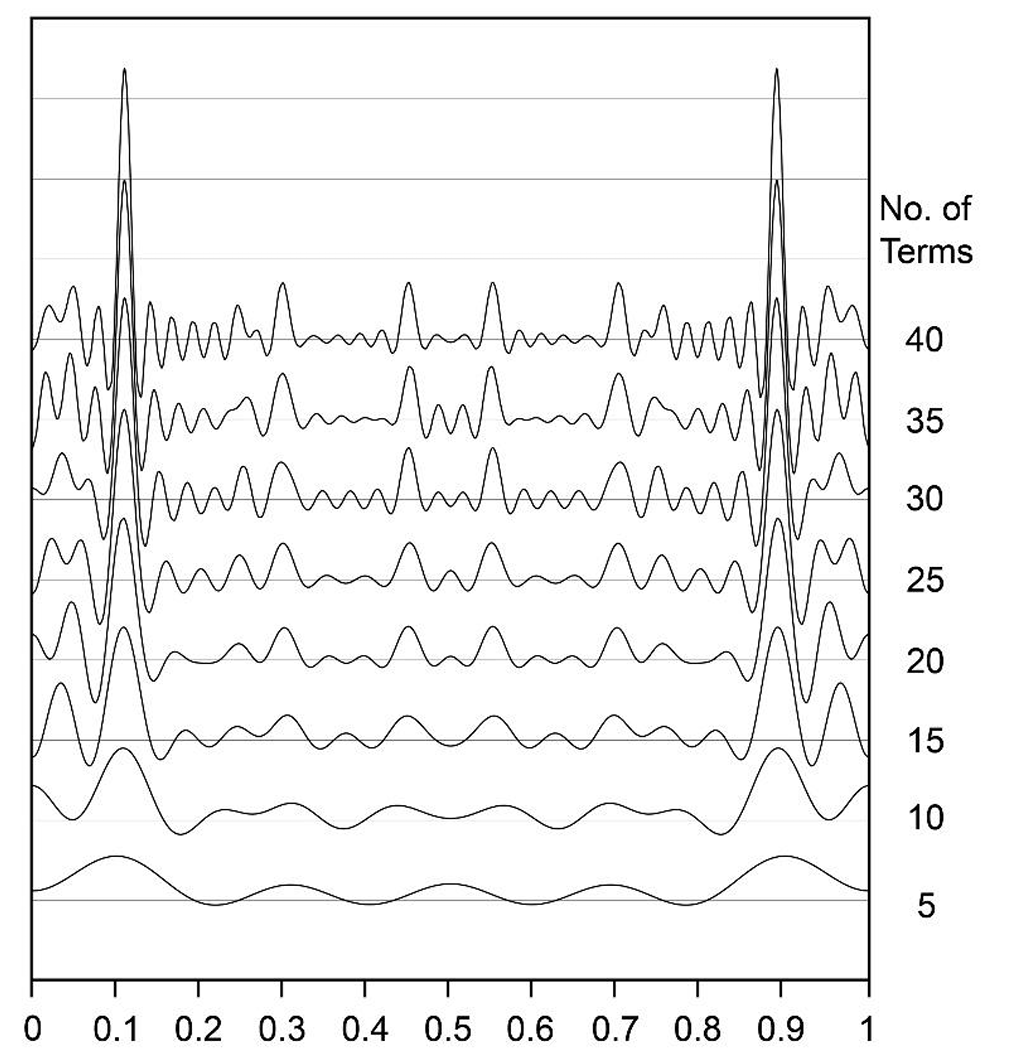
\includegraphics[width=0.5\textwidth]{Termination_error.png}
        \caption{Fourier synthesis of electron density in caesium picrate \(\mathrm{Cs[C_6H_2(NO_2)_3O]}\) as number of terms increases.}
        \label{Fig:Termination_error}
    \end{figure}

    Let's consider the example of caesium picrate \(\mathrm{Cs[C_6H_2(NO_2)_3O]}\), projected onto the \(x\) axis. \Cref{Fig:Termination_error} shows progressively larger number of \(E(h)\) values included in the Fourier synthesis of electron density. We see with only five terms included in the sum, only Cs atoms at \(x\approx 0.1\) and \(x\approx 0.9\) can be observed, and the C, N and O atoms are not resolved. As more terms are included, the lighter atoms become visible, and the large Cs peaks also becomes sharper. However, the Cs peaks are also surrounded by large negative ripples, which arises due to the series termination errors. These remain strong even when 40 terms are included in the series, only disappearing when the number of terms exceeds 100. Therefore, we are likely to observe negative electron density regions around heavy atoms even when our phases are correct. Consequently, any method relying on the non-negativity of electron density may falsely rule out the correct phases combinations.

    The solution is also simple. If heavy atoms are present, then Patterson function plus phase determining methods based on heavy atoms would be ideal. Direct method and heavy atom based methods are perfectly complementary.
    
    Moreover, for molecules like proteins when there are no particularly heavy atoms and the unit cells are large, there might be no particularly strong peaks, and the intensities are measured at low resolutions. For them, multiple isomorphous replacement, multiple anomalous scattering or (most commonly) single anomalous scattering would be used.

    \subsection{Dual-Space Methods}
    In fact, most chemical structures solved today use neither the Patterson function nor direct methods. Instead, modern computing power enables application of the following algorithm called the \textit{dual-space method}.

    \begin{enumerate}
        \item Produce a random phase \(\Phi(hkl)\) for each measured \(F(hkl)\).
        \item Generate \(\rho(x,y,z)\) at points on a defined grid within the unit cell by the inverse Fourier transform using measured \(\abs{F(hkl)}\) and current \(\Phi(hkl)\).
        \item For any grid point with negative \(\rho(x,y,z)\), multiply the value by \(-1\).
        \item Calculate new \(F(hkl)\) by the Fourier transform of \(\rho(x,y,z)\).
        \item Replace the current phase set with the \(\Phi(hkl)\) values obtained in step 4, then return to step 2.
    \end{enumerate}

    The above operation will converge to a \(\rho(x,y,z)\) which is necessarily non-negative. We would repeat the procedure many times from different initial sets and to assess which of the converged solutions is the most likely to be correct.

    The fundamental basis of the dual space method is clearly the non-negativity of electron density, and the process of flipping negative \(\rho(x,y,z)\) is an example of \textit{density modification}, meaning modifying the calculated electron density to conform to our expectations. The established principle of atomicity can also be applied to the structure at some defined frequency during the iteration. This is achieved by identifying a number of maxima in \(\rho\) and replacing them by isolated spherical electron densities at these positions.

    An additional benefit of dual-space method is that it does not require the symmetry of the crystal structure to be firmly established. They are usually applied to the whole unit cell content.

    \newpage
    \section{Structure Refinement and Other Diffraction Methods}
    The methods described in previous sections generally produce only an approximate model to the structure under investigation, commonly referred to as a \textit{trial structure}. Atoms may deviate from their true positions quite significantly, and some atoms may remain to be found. In order to complete the model, it is necessary to refine the structure. We will provide a brief outline here.

    \subsection{Residual Minimisation}
    As the observed \(\abs{F(hkl)}\) are known functions of the atomic coordinates, the latter can be refined using least-squares methods. The quantity to be minimised is the \textit{residual}
    \begin{equation}
        R=\sum_{hkl}w_{hkl}[\abs{F_{\text{obs}}(hkl)}^2-\abs{F_{\text{calc}}(hkl)}^2]^2\,,
    \end{equation}
    where \(w_{hkl}\) is a weighting factor expressing the accuracy of individual \(\abs{F_{\text{obs}}(hkl)}\) values derived during measurements.

    However, this is not as simple as it seems. The structure factor equation is not linear, so it is not possible to apply straightforward least-squares methods. We need to \textit{linearise} the equation by considering the \textit{atomic shifts} \(\delta x_n = x_n'-x_n\), and compute the best value of shifts for a particular set of coordinates. We can iterate until the optimal shifts become small. Like any optimisation processes, we want to converge to the global minimum of the residual, but as ever, we are likely to get stuck at a local minimum during optimisation. We then need to use our chemical intuition e.g. whether some bond lengths or coordination environment are suspicious to identify the true structure.

    \subsection{Locating the Atoms}
    In accordance with the Independent Atom Model, the image of \(\rho(x,y,z)\) must then be interpreted to obtain coordinates for each atom. Atoms are considered to lie at the centroids of concentrated regions of electron density. The accuracy of the atomic positions must therefore depend on the quality of the electron density map. The image of \(\rho(x,y,z)\) is influenced by the number of terms included in the Fourier synthesis, and the derived atomic coordinates are therefore very much dependent on the resolution of the analysis.
    
    Examples are shown in \cref{Fig:Resolution} for a section of the electron density map through the benzene ring of the molecule sulfathiazole. At the exceptionally high resolution of \(0.46\,\text{\AA}\), the atoms are very clearly defined, and their centres can be identified with confidence. However, note that it is not entirely obvious where the H atoms lie. At \(1.20\,\text{\AA}\) resolution, the atoms of the benzene ring merge effectively into a continuous feature, and it is more difficult to define each atomic centre. For the four C(H) atoms, the electron density appears to protrude outward in the direction where H atom is expected. Hence, defining the C atom coordinates at the centroid of these distorted features is likely to result in a distorted geometry for the benzene ring. A more typical resolution for a molecular crystal structure is \(0.85\,\text{\AA}\), which can be seen to produce relatively well defined atoms. Nonetheless, it should be clear that the accuracy of the final atomic coordinates can be limited for lower resolution crystal structures, and great care should be taken when interpreting derived bond distances and angles.

    \begin{figure}
        \centering
        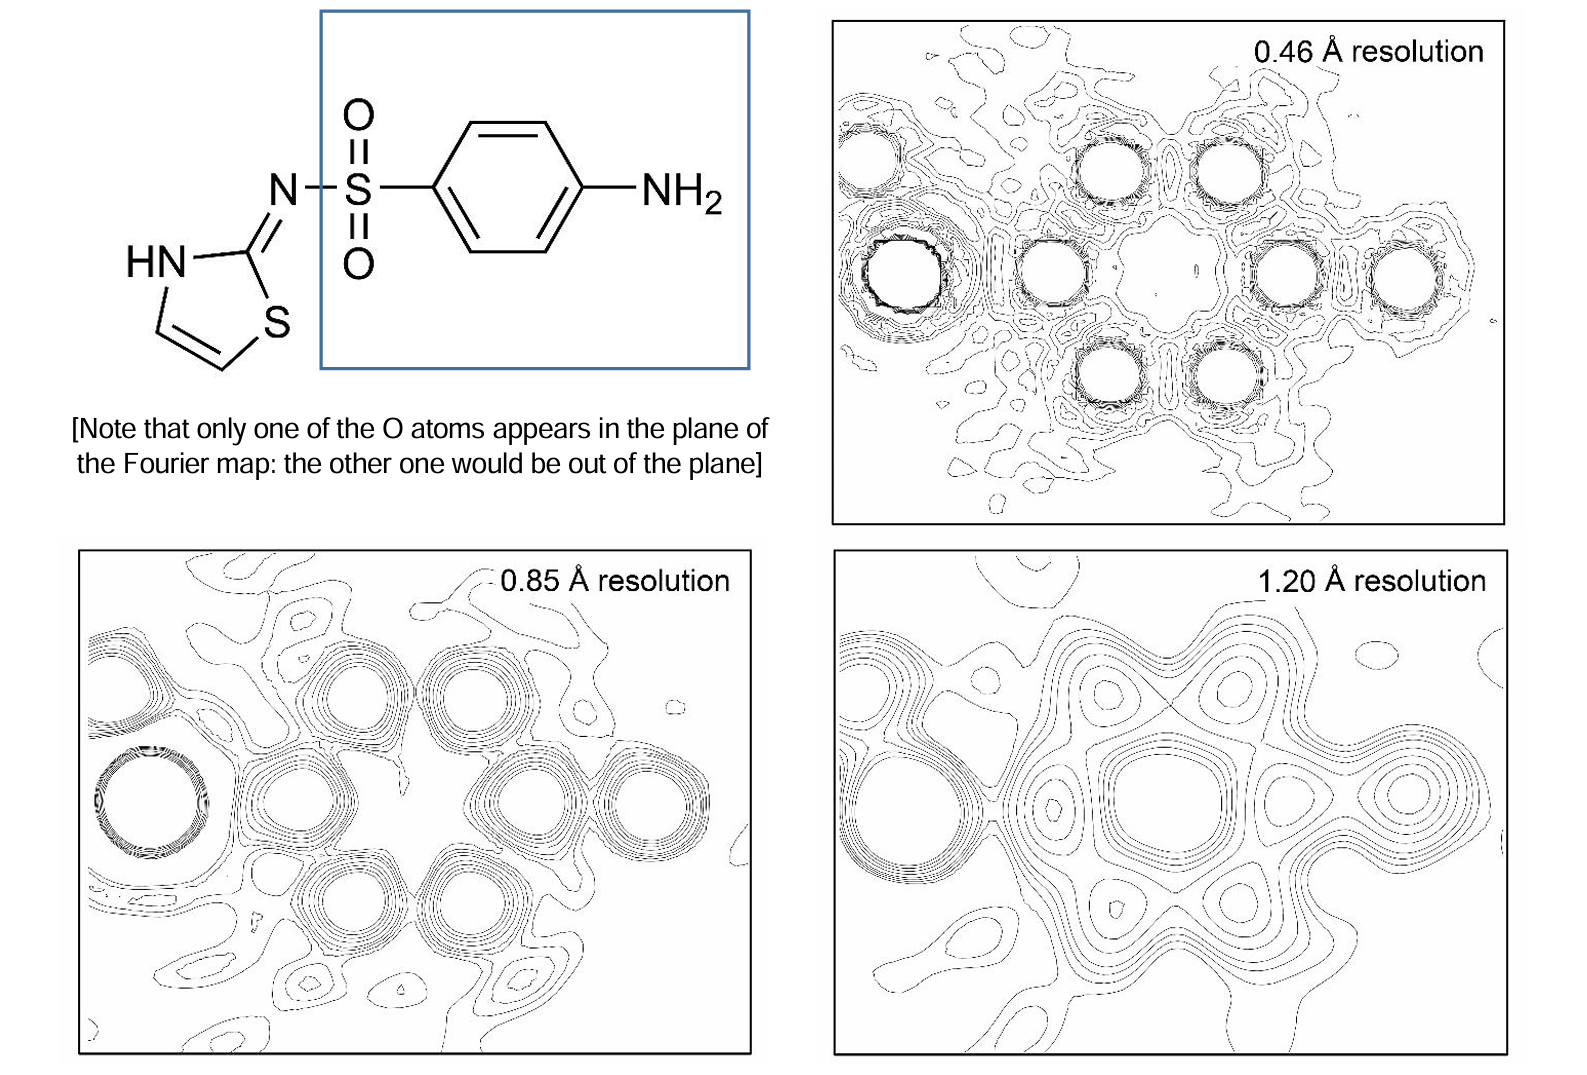
\includegraphics[width=0.9\textwidth]{Resolution.png}
        \caption{Electron density map of sulfathiazole at different resolutions.}
        \label{Fig:Resolution}
    \end{figure}

    \subsection{The Difference Density}
    We can define the \textit{difference density} as the inverse Fourier transform of the difference between the observed and calculated \(\abs{F(hkl)}\) values
    \begin{equation}
        \rho_{\text{D}}(x,y,z)=\mathcal{F}^{-1}\left[(\abs{F_{\text{obs}}(hkl)}-\abs{F_{\text{calc}}(hkl)})\exp[\ii\Phi_{\text{calc}}(hkl)]\right]\,,
    \end{equation}
    where \(\abs{F_{\text{calc}}(hkl)}\) and \(\Phi_{\text{calc}}(hkl)\) are calculated from the current trial structure.

    The resulting difference density is interpreted as the difference between the correct structure and the trial structure. If our trial structure is absolutely correct, the difference density should be identically zero. Normally, \(\rho_{\text{D}}\) has some definite characteristics:
    \begin{itemize}
        \item \textit{Positive peaks}: this arises if an atom has been omitted from the trial structure. Towards the end of a refinement, this is usually the hydrogen atom. It is very difficult to find H atoms in an image of the actual electron density, \(\rho(x,y,z)\), because it is usually submerged in the noise of series termination error, especially in the presence of other heavy atoms. The H atoms are usually more clearly seen on the difference density since both \(\abs{F_{\text{obs}}(hkl)}\) and \(\abs{F_{\text{calc}}(hkl)}\) are subjected to termination errors, so the subtraction will cancel them out to some extent.
        \item \textit{Positive and negative peaks adjacent to an atom in the trial structure}: this will arise if the atom is not quite at the right position. It can be rectified by moving the atom in the direction of the maximum \(\rho_{\text{D}}\) gradient.
        \item \textit{Hollow peaks at an atom position in the trial structure}: a negative peak surrounded by a pronounced positive rim will occur if the trial structure is effectively more `dense' than in the real structure. This often arises when there is a need to optimise the atomic displacement parameter. This is mentioned further below.
    \end{itemize}

    Since \(\rho(x,y,z)\) is always subject to series termination errors, we cannot expect the difference density ever to be zero. There will always be ``Fourier ripples'' around particularly heavy atoms, which might be quite substantial (say \(1e\text{\AA}{}^{-3}\)). The crucial point is that a completed structure refinement should not have any remaining features in \(\rho_{\text{D}}\) that are indicative of missing atoms, i.e. a peak of \(1e\,\text{\AA}{}^{-3}\) within \(0.5\,\text{\AA}\) of a heavy atom is likely to be just a Fourier ripple, but a peak of \(1e\,\text{\AA}{}^{-3}\) at a distance of \textit{ca} \(1\,\text{\AA}\) from an O atom making only one other bond is clearly the H atom of an OH group. Hence, some chemical understanding is also required to interpret crystallographic results.

    \subsection{Atomic Displacement Parameters}
    Atomic displacement parameters, ADPs, were mentioned in the discussion of atomic scattering factors. The ADPs can be viewed to ``modulate'' the atomic scattering factors to account for thermal vibration or static displacement (where an atom might take slightly different positions within different unit cells).

    ADPs should always be positive and serve to decrease an atom's contribution in the structure factor equation. They are visualised by representing the atom as a sphere (for an isotropic ADP) or ellipsoid (for an anisotropic ADP) scaled to the size of the numerical parameters. For a given crystal structure, it is reasonable to expect, and generally observed, that all atoms have displacement ellipsoids/spheres of a similar size. Anomalous ADPs are indicative of atoms that may have been assigned the wrong atom type. During a structure refinement, the atom type is defined by the choice of atomic scattering factor, which is then fixed during a given refinement run. The ADPs, on the other hand, are numerical parameters that can be refined during the least-squares process, and can respond to an incorrect choice of atoms. If an atomic site is assigned an atom type with too many electrons, the ADPs will become large to diminish the atomic scattering factor. Conversely, if an atomic site is assigned as an atom site with too few electrons, the ADPs will become small so that they do not apply any significant modulating effect. In extreme cases, ADPs can refine to negative values (in the anisotropic case, the displacement tensor becomes ``non-positive definite''), which makes no physical sense and is not acceptable in a crystallographic result.

    \subsection{H atoms}
    It has been mentioned that H atoms can be difficult to locate in \(\rho(x,y,z)\) because they only have one electron. An additional point to consider is where the H atom actually is. The one electron of H will almost always be involved in a covalent bond, so the maximum electron density in a \(\mathrm{C-H}\) bond (for example) will be somewhere between the C atom and the proper nuclear position of the H atom. Since atomic positions are deduced from maxima in \(\rho(x,y,z)\), H atoms will be placed too close to the atom to which they are bonded, i.e. bond lengths to H in X-ray crystal structures are always systematically too short.
    
    Often we know enough about molecular structure to know where H atoms should be, so we can just place H atoms in calculated positions. However, we still have to place them in the ``wrong'' (shortened) positions because we are still trying to fit an electron density map. True H atom positions can be estimated by normalising \(\mathrm{X-H}\) bonds to values obtained from neutron diffraction.

    \subsection{Assessing the Quality of the Results}
    When the refinement has been completed, the final result of the structure determination is commonly expressed by two different normalised residuals:
    \begin{align}
        wR2&=\left(\frac{\sum_{hkl}w_{hkl}\left[\abs{F_{\text{obs}}(hkl)}^2-\abs{F_{\text{calc}}(hkl)}^2\right]^2}{\sum_{hkl}w_{hkl}\left[\abs{F_{\text{obs}}(hkl)}^2\right]^2}\right)^{1/2}\\
        R1&=\frac{\sum_{hkl}\abs{\abs{F_{\text{obs}}(hkl)}-\abs{F_{\text{calc}}(hkl)}}}{\sum_{hkl}\abs{F_{\text{obs}}(hkl)}}\,.
    \end{align}
    The first of these is a root-mean-squared value derived directly from the refined residual, while the second is based on absolute differences between the structure factor magnitudes. The \(wR2\) measure is preferred because it can include all intensity data. \(R1\) will require weak \(\abs{F}\) values below a minimum threshold (typically greater than 3 times the estimated error) to be ignored because of the difficulties assessing their accuracy.

    For a chemical crystal structure, \(wR2\) is typically in the range \(0.10\sim 0.20\). \(R1\) values are always smaller, typically in the range \(0.05\sim 0.10\). There may be reasons why \(R\)-factors could be larger than these quoted values, for example a very weakly diffracting crystal (producing noisy intensities), or substantial disorder, where atoms may not correspond to the expectations of perfect long-range order in a single crystal. Hence, \(R\)-factors alone do not always tell the full story. To assess a crystal structure, it is important also to compare it to expectations based on physical and chemical sense.

    \subsection{Neutron and Electron Diffraction}
    This course has focused mainly on X-ray diffraction because X-rays are most commonly used for chemical characterisation, particularly in ``home'' laboratories. The same principles apply of course to other radiation sources. Neutrons have long been used to complement X-ray diffraction analyses, and electron diffraction is also now emerging as a practical technique to study micro- and nano-crystalline materials. 

    \subsubsection{Neutron Diffraction}
    Although they are commonly regarded as particles, neutrons have a wave-like character (as all the particles) and are also diffracted by matter. Thermal neutrons from a reactor have a kinetic energy given by:
    \begin{equation}
        E=\frac{1}{2}mv^2\approx k_B T=4\times 10^{-21}\unit{J}
    \end{equation}
    at room temperature. This corresponds roughly to a velocity of \(2,200\unit{m}\unit{s}^{-1}\), and hence a wavelength of about \(1.8\,\text{\AA}\), which is eminently suitable for diffraction studies.

    Neutron diffraction has some distinct advantages over X-ray diffraction:
    \begin{enumerate}
        \item Neutrons are mainly scattered by atomic nuclei, which are very small. Consequently peaks in either a Patterson function or a ``nuclear density'' map produced by the inverse Fourier transform will be very sharp, making interpretation easier.
        \item For X-ray diffraction, the scattering power of an atom is roughly proportional to its atomic number. This means that light atoms, particularly H, may be difficult to identify and refine. In neutron diffraction, the scattering power of a nucleus depends on the nuclear energy levels, which vary in an almost random way, even among isotopes of the same element. Consequently some light atoms scatter neutrons more strongly than heavy ones. The most important case involves the scattering from isotopes of H, which is very strong from 2H (deuterium). Neutron diffraction is therefore a good way to locate the true positions of H atoms by experiment.
        
        The random variation of neutron scattering powers can be exploited in other ways. For example, it is difficult using X-ray diffraction to distinguish between atoms with very similar atomic number because they have almost identical scattering power. A classic example is Si and Al in a zeolite structure. For neutrons however, their scattering powers are different, and they can be easily distinguished.
        \item Neutrons have spin, and can therefore interact with the local magnetic field produced by an unpaired electron. If unpaired electrons are present, the atomic scattering factor for neutrons can be written as:
        \begin{equation}
            f_{\text{neutron}} = f_{\text{nuclear}} + f_{\text{magnetic}}\,. 
        \end{equation}
        When we record an experimental set of diffracted intensities using neutrons, we are recording the effects of both magnetic and nuclear components of the scattering. If the basic structure is known (usually from a preliminary X-ray measurement), we can calculate a type of ``difference density'' using \(\abs{F_{\text{calc}}(hkl)}\) and \(\Phi_{\text{calc}}(hkl)\) values which are deduced from the atomic parameters using the nuclear scattering factors only. The features which show up in the difference density then highlight parts of the structure where magnetic electrons are present. This difference density, which has the form:
        \begin{equation}
            \rho_{\text{magnetic}}(x,y,z)=\mathcal{F}^{-1}\left[(\abs{F_{\text{obs}}(hkl)}-\abs{F_{\text{calc}}(hkl)})\exp[\ii\Phi_{\text{calc}}(hkl)]\right]\,,
        \end{equation}
        is normally referred to as the \textit{magnetic scattering density}. 
    \end{enumerate}

    Although they have these clear advantages, neutrons also have two important disadvantages which restrict their use:
    \begin{enumerate}
        \item Thermal neutrons require a nuclear reactor for their generation. Consequently they are only available in certain specialised central facilities, to which applications for beam time must be made and where complicated experimental arrangements for ``one-off'' or speculative experiments are not generally possible.
        \item Neutron scattering is almost two orders of magnitude weaker than X-ray scattering. Consequently, to record acceptable diffracted intensities usually requires a larger sample. In the case of powder diffraction, this is not too much of a problem, but most \textit{ab initio} structure solution requires single crystals, and these are frequently very difficult, if not impossible, to grow in the sizes required for neutron work. This is particularly true for materials such as proteins. 
    \end{enumerate}

    \subsubsection{Electron Diffraction}
    Accelerated electrons also have significant wave-like character. For a representative accelerating voltage of \(200 \unit{keV}\) in an electron microscope, the wavelength is about \(0.025\,\text{\AA}\); considerably shorter than X-ray wavelengths used in laboratory diffraction instruments but still in the region to permit diffraction studies.

    The main benefit of using electrons is that it allows diffraction data to be collected from nano-crystalline samples, with volume two or three orders of magnitude smaller than those required for lab-based X-ray measurements. This is possible due to the strong coulomb interaction between the electron beam and the sample. However, there are practical drawbacks, namely that measurements are required to be made in a vacuum, and have generally been implemented with electron microscopes that limit sample movement and therefore cannot access all areas of reciprocal space. In addition, exposure to intense electron beams can lead to rapid sample decomposition, especially for organic molecules. These practical matters have generally limited the application of electron diffraction compared to X-ray diffraction. Some of them are now starting to be overcome by dedicated electron diffraction instruments and cryo-cooling of samples, \textit{etc.}, and the technique is likely to grow significantly in the coming years.

    The particularly strong scattering of electrons leads to challenges in data interpretation. In particular, recall from the initial discussion that we developed the Fourier transform relationship under the assumption that the total scattering is small compared to the strength of the incident beam. For electrons, we cannot assume that the scattering is small compared to the incident beam, so we have to deal with \textit{dynamical scattering theory}, which takes into account multiple scattering effects (i.e. re-scattering of the scattered beams). Practically, it is helpful to minimise multiple scattering in electron diffraction by using samples that are as thin as possible (with the drawback that this is likely to accelerate sample decomposition), but it still cannot be ignored during structure determination and refinement procedures.
    
    For many years, software used for X-ray structure solution and refinement has simply been applied to electron diffraction data, and it has been accepted that the results will be generally worse than those obtained using X-rays (an acceptable price to pay for being able to look at very small samples). In the last few years, however, effective software implementing the full dynamical theory has started to emerge. The calculations are very much more intensive than for X-rays, so cycles of refinement may reach hours rather than seconds for X-rays. The computational cost obviously increases with structure size, and macromolecular refinements are not in reach in the immediate future. However, the methods have produced promising results for small-molecule structures, including effective identification of H atoms and absolute structure determination.




\end{document}